%% This is the ctufit-thesis example file. It is used to produce theses
%% for submission to Czech Technical University, Faculty of Information Technology.
%%
%% Get the newest version from
%% https://gitlab.fit.cvut.cz/theses-templates/FITthesis-LaTeX
%%
%%
%% Copyright 2021, Eliska Sestakova and Ondrej Guth
%%
%% This work may be distributed and/or modified under the
%% conditions of the LaTeX Project Public Licenese, either version 1.3
%% of this license or (at your option) any later version.
%% The latest version of this license is in
%%  https://www.latex-project.org/lppl.txt
%% and version 1.3 or later is part of all distributions of LaTeX
%% version 2005/12/01 or later.
%%
%% This work has the LPPL maintenance status `maintained'.
%%
%% The current maintainer of this work is Ondrej Guth.
%% Contact ondrej.guth@fit.cvut.cz for bug reports.
%% Alternatively, submit bug reports into the tracker at
%% https://gitlab.fit.cvut.cz/theses-templates/FITthesis-LaTeX/issues
%%
%%

%%%%%%%%%%%%%%%%%%%%%%%%%%%%%%%%%%%%%%%%%
% CLASS OPTIONS
% language: czech/english/slovak
% thesis type: bachelor/master/dissertation
%%%%%%%%%%%%%%%%%%%%%%%%%%%%%%%%%%%%%%%%%
\documentclass[english,bachelor,unicode]{ctufit-thesis}

%%%%%%%%%%%%%%%%%%%%%%%%%%%%%%%%%%
% FILL IN THIS INFORMATION
%%%%%%%%%%%%%%%%%%%%%%%%%%%%%%%%%%
\ctufittitle{Physical Unclonable Functions on ESP32} % replace with the title of your thesis
\ctufitauthorfull{Ondřej Staníček} % replace with your full name (first name(s) and then family name(s) / surname(s)) including academic degrees
\ctufitauthorsurnames{Staníček} % replace with your surname(s) / family name(s)
\ctufitauthorgivennames{Ondřej} % replace with your first name(s) / given name(s)
\ctufitsupervisor{Ing.\,Jiří Buček,\,Ph.D.} % replace with name of your supervisor/advisor (include academic degrees)
\ctufitdepartment{Department of Computer Systems} % replace with the department of your defence % TODO neni to informacni bezpecnost katedra?
\ctufityear{2022} % replace with the year of your defence
\ctufitdeclarationplace{Prague} % replace with the place where you sign the declaration
\ctufitdeclarationdate{\today} % replace with the date of signature of the declaration

\ctufitabstractENG{
    This thesis analyzes the possibility of implementing a \gls{sram} \gls{puf} on the ESP32 microcontroller.
    
    First, literature research on the topic of \glspl{puf} is provided with focus on \gls{sram} \glspl{puf}. A discussion on which properties the \gls{sram} \glspl{puf} possess is presented.

    Two power-control methods of \gls{sram} memory on the ESP32 are proposed. An analysis of behavior of startup \gls{sram} bit values depending on operating temperature and power-off time is conducted for both methods. Their suitability for the \gls{puf} implementation is discussed based on the experimental results.

    Then, an implementation of \gls{sram} \gls{puf} with stable response reconstruction is presented. Two different bit preselection methods are tested and a simple repetition \gls{ecc} is used to stabilize the responses. The presented \gls{puf} design combines the two power-control methods to achieve faster and more reliable response extraction.

    Reliability testing revealed that it is possible to reach 100 \% success rate of response reconstruction across the temperature range of -40 to +70~°C. The responses can be used as cryptographic keys to secure the ESP32 platform. Finally, the proposed \gls{puf} design is implemented in an easy-to-use ESP32 library.
}

\ctufitabstractCZE{
    Tato práce zkoumá možnost implementace fyzicky neklonovatelné funkce (\gls{puf}) na základě statické paměti (\gls{sram}) na mikrokontroléru ESP32.

    Nejprve je provedena rešerše o problematice \gls{puf} se zaměřením na \gls{sram} \gls{puf}\@. Také jsou popsány vlastnosti \gls{sram} \gls{puf}u.

    Jsou představeny dvě metody kontroly napájení \gls{sram} paměti. Pro obě je provedena analýza chování neinicializovaných \gls{sram} dat dle operační teploty a doby vypnutí. Na základě těchto výsledků je posouzena vhodnost jejich využití.

    Poté je představena implementace \gls{sram} \gls{puf}u se spolehlivou rekonstrukcí odpovědi. Dvě různé metody výběru stabilních bitů a opakovací samoopravný kód jsou použity ke stabilizaci odpovědí. Tato implementace kombinuje obě představené metody kontroly napájení paměti, címž dosahuje rychlejší a spolehlivější extrakce odpovědí.

    Testování spolehlivosti odhalilo, že je možné dosáhnout 100~\% úspěšnosti rekonstrukce odpovědí při teplotách od -40 do +70~°C. Tyto odpovědi je možné použít jako kryptografické klíče k zabezpečení ESP32. Nakonec je tento návrh \gls{sram} \gls{puf}u implementován jako snadno použitelná ESP32 knihovna.
}


\ctufitkeywordsENG{ESP32, physical unclonable functions, static random access memory, key generation, error correction codes, hardware security}
\ctufitkeywordsCZE{ESP32, fyzicky neklonovatelné funkce, statická paměť, samoopravné kódy, generování klíčů, hardwarová bezpečnost}
%%%%%%%%%%%%%%%%%%%%%%%%%%%%%%%%%%
% END FILL IN
%%%%%%%%%%%%%%%%%%%%%%%%%%%%%%%%%%

%%%%%%%%%%%%%%%%%%%%%%%%%%%%%%%%%%
% CUSTOMIZATION of this template
% Skip this part or alter it if you know what you are doing.
%%%%%%%%%%%%%%%%%%%%%%%%%%%%%%%%%%

\RequirePackage{iftex}[2020/03/06]
\iftutex % XeLaTeX and LuaLaTeX
    \RequirePackage{ellipsis}[2020/05/22] %ellipsis workaround for XeLaTeX
\else
    \RequirePackage[utf8]{inputenc}[2018/08/11] %this file encoding
    \RequirePackage{lmodern}[2009/10/30] % vector flavor of Computer Modern font
\fi

% hyperlinks
% \RequirePackage[pdfpagelayout=TwoPageRight,colorlinks=false,allcolors=decoration,pdfborder={0 0 0.1}]{hyperref}[2020-05-15]

% uncomment the following to hide all hyperlinks
\RequirePackage[pdfpagelayout=TwoPageRight,hidelinks]{hyperref}[2020-05-15]

\RequirePackage{pdfpages}[2020/01/28]

\setcounter{secnumdepth}{4} % numbering sections; 4: subsubsection



%%%%%%%%%%%%%%%%%%%%%%%%%%%%%%%%%%
% CUSTOMIZATION of this template END
%%%%%%%%%%%%%%%%%%%%%%%%%%%%%%%%%%


%%%%%%%%%%%%%%%%%%%%%%
% DEMO CONTENTS SETTINGS
% You may choose to modify this part.
%%%%%%%%%%%%%%%%%%%%%%
\usepackage{dirtree}
\usepackage{lipsum,tikz}
\usepackage{csquotes}
\usepackage[style=iso-numeric]{biblatex}
\addbibresource{text/bib-database.bib}
\usepackage{listings} % typesetting of sources
% \usepackage{minted} % typesetting of sources

%%%%%%%%%%%%%%%%%%%%%%%%%%%%%%%%%%
% OWN PACKAGES
%%%%%%%%%%%%%%%%%%%%%%%%%%%%%%%%%%

% TODO a SRAM or an SRAM???

%\usepackage{parskip}
\usepackage{dirtytalk}
\usepackage{graphicx}
\usepackage{float}
\usepackage{mathtools}
%\usepackage[bottom]{footmisc} % footnote hyperref links do not work with this
\usepackage{enumitem}
\usepackage[nopostdot,style=super,nonumberlist,nogroupskip,toc]{glossaries}
\usepackage{subcaption}
\usepackage{nameref}
\usepackage{booktabs}
\usepackage[dvipsnames]{xcolor}

\interfootnotelinepenalty=10000
\makeglossaries{}
\emergencystretch=1em
\setlist{leftmargin=9.5mm}

\hypersetup{
    pdftitle={Physical unclonable functions on ESP32},
    pdfauthor={Ondřej Staníček},
    pdfkeywords={ESP32, physical unclonable functions, static random access memory, error correction codes, hardware security}
}

\definecolor{dark-gray}{gray}{0.30}

\lstdefinestyle{customc}{
  belowcaptionskip=1\baselineskip,
  breaklines=true,
  frame=L,
  xleftmargin=\parindent,
  language=C++,
  showstringspaces=false,
  basicstyle=\small\ttfamily,
  keywordstyle=\bfseries\color{RawSienna},
  commentstyle=\itshape\color{dark-gray},
  identifierstyle=\color{Black},
  stringstyle=\color{OliveGreen}
}

\captionsetup[lstlisting]{position=bottom,justification=centering,margin=0.5cm}

%%%%%%%%%%%%%%%%%%%%%%%%%%%%%%%%%%
% OWN PACKAGES END
%%%%%%%%%%%%%%%%%%%%%%%%%%%%%%%%%%

%theorems, definitions, etc.
\theoremstyle{plain}
\newtheorem{theorem}{Theorem}
\newtheorem{lemma}[theorem]{Lemma}
\newtheorem{corollary}[theorem]{Corollary}
\newtheorem{proposition}[theorem]{Proposition}
\newtheorem{definition}[theorem]{Definition}
\theoremstyle{definition}
\newtheorem{example}[theorem]{Example}
\theoremstyle{remark}
\newtheorem{note}[theorem]{Note}
\newtheorem*{note*}{Note}
\newtheorem{remark}[theorem]{Remark}
\newtheorem*{remark*}{Remark}
\numberwithin{theorem}{chapter}
%theorems, definitions, etc. END
%%%%%%%%%%%%%%%%%%%%%%
% DEMO CONTENTS SETTINGS END
%%%%%%%%%%%%%%%%%%%%%%
\setacronymstyle{long-short}
\loadglsentries{glossary.tex}
\glsaddall

\begin{document} 
\frontmatter\frontmatterinit % do not remove these two commands


\includepdf{assignment-include.pdf} % replace that file with your thesis assignment provided by study office

\thispagestyle{empty}\cleardoublepage\maketitle % do not remove these three commands

\imprintpage % do not remove this command

\tableofcontents % do not remove this command
%%%%%%%%%%%%%%%%%%%%%%
% list of other contents: figures, tables, code listings, algorithms, etc.
% add/remove commands accordingly
%%%%%%%%%%%%%%%%%%%%%%
\listoffigures % list of figures
\begingroup
\let\clearpage\relax
\listoftables % list of tables
\lstlistoflistings % list of source code listings generated by the listings package
% \listoflistings % list of source code listings generated by the minted package
\endgroup
%%%%%%%%%%%%%%%%%%%%%%
% list of other contents END
%%%%%%%%%%%%%%%%%%%%%%

%%%%%%%%%%%%%%%%%%%
% ACKNOWLEDGMENT
% FILL IN / MODIFY
% This is a place to thank people for helping you. It is common to thank your supervisor.
%%%%%%%%%%%%%%%%%%%
\begin{acknowledgmentpage}
	Chtěl bych poděkovat především sit amet, consectetuer adipiscing elit. Curabitur sagittis hendrerit ante. Class aptent taciti sociosqu ad litora torquent per conubia nostra, per inceptos hymenaeos. Cras pede libero, dapibus nec, pretium sit amet, tempor quis. Sed vel lectus. Donec odio tempus molestie, porttitor ut, iaculis quis, sem. Suspendisse sagittis ultrices augue.
\end{acknowledgmentpage} 
%%%%%%%%%%%%%%%%%%%
% ACKNOWLEDGMENT END
%%%%%%%%%%%%%%%%%%%


%%%%%%%%%%%%%%%%%%%
% DECLARATION
% FILL IN / MODIFY
%%%%%%%%%%%%%%%%%%%
% INSTRUCTIONS
% ENG: choose one of approved texts of the declaration. DO NOT CREATE YOUR OWN. Find the approved texts at https://courses.fit.cvut.cz/SFE/download/index.html#_documents (document Declaration for FT in English)
% CZE/SLO: Vyberte jedno z fakultou schvalenych prohlaseni. NEVKLADEJTE VLASTNI TEXT. Schvalena prohlaseni najdete zde: https://courses.fit.cvut.cz/SZZ/dokumenty/index.html#_dokumenty (prohlášení do ZP)
% TODO licence pro volne uziti, zeptat se bucka?
\begin{declarationpage}
I hereby declare that the presented thesis is my own work and that I have cited all
sources of information in accordance with the Guideline for adhering to ethical
principles when elaborating an academic final thesis.
I acknowledge that my thesis is subject to the rights and obligations stipulated by the
Act No. 121/2000 Coll., the Copyright Act, as amended. In accordance with Article 46 (6)
of the Act, I hereby grant a nonexclusive authorization (license) to utilize this thesis,
including any and all computer programs incorporated therein or attached thereto and
all corresponding documentation (hereinafter collectively referred to as the “Work”), to
any and all persons that wish to utilize the Work. Such persons are entitled to use the
Work for non-profit purposes only, in any way that does not detract from its value. This
authorization is not limited in terms of time, location and quantity.
\end{declarationpage}
%%%%%%%%%%%%%%%%%%%
% DECLARATION END
%%%%%%%%%%%%%%%%%%%

\printabstractpage % do not remove this command

\printglossary[type=\acronymtype,title={List of Abbreviations}]

\mainmatter\mainmatterinit % do not remove these two commands

%%%%%%%%%%%%%%%%%%%
% THE THESIS
% MODIFY ANYTHING BELOW THIS LINE
%%%%%%%%%%%%%%%%%%%

\glsresetall
\glsunset{cpu}
\glsunset{uart}

%---------------------------------------------------------------
\chapter{Introduction}
%---------------------------------------------------------------

%--------------------------------
\section{Objectives of the thesis}
%--------------------------------

%The research part of the thesis will describe what is a \gls{puf} and what are the uses of this technology, focusing mainly on \gls{sram} based \glspl{puf}. Furthermore, the parameters used to evaluate performance of \glspl{puf} will be defined.

%The main objective of the practical part of this thesis is to analyze the possibility of implementing a \gls{sram} based \gls{puf} on the ESP32 family of microcontrollers. This means finding a suitable mechanism of \gls{sram} power control and establishing a way to gather \gls{puf} response data reliably. Next, stability and uniqueness of the obtained \gls{puf} data using the defined parameters will be evaluated. An analysis of the \gls{sram} data depending on different operating temperature and power-off time will be performed as well.

%The next goal will be to implement a simple \gls{sram} based \gls{puf} based on the knowledge gained in the previous experiments. Several different models of devices from the ESP32 family will be used to test the function and performance of the resulting \gls{puf} implementation.

\section{Structure of the thesis}


%---------------------------------------------------------------
\chapter{Physical unclonable functions}
%---------------------------------------------------------------

%--------------------------------
\section{PUF description}
%--------------------------------

As \glspl{puf} are the main subject of this thesis, it is important to provide a thorough explanation of what a \gls{puf} is, what types and classes exist and what are
the applications of this technology.

Since more and more types of \glspl{puf} are being invented, it turns out that creating a generalizable description is not a straightforward task. A dictionary definition of a \gls{puf} could be expressed as: \say{a PUF is an expression of an inherent and unclonable instance-specific feature of a physical object}. One can imagine a \gls{puf} being an object's fingerprint in a comparable way to how humans have their own fingerprints.\cite{Maes2013}

The first concept of \gls{puf} was proposed by Pappu in 2001. He used the term \gls{powf}, which he described as a function operating on a physical system that could be easily computed but not easily inverted.\cite{Pappu2001} The first mention of the term \gls{puf} was by Gassend et al.\ in 2002. He talks about \glspl{prf} and a \gls{puf} implementation using \glspl{fpga}.\cite{Gassend2002}

As \gls{puf} is a function, it has inputs and outputs. However, it is not a function in a true mathematical way. It could be described as a procedure performed on a particular device. Its inputs consist of a challenge and a physical state of the device. Given the input, the \gls{puf} produces an output (called a response). Together, they form challenge-response pairs.   

A hugely important property of \glspl{puf} is unclonability. It is achieved by the physical state of the device which acts as the input to the function and influences the responses produced by the \gls{puf}. The concrete details of the physical state used is what distinguishes different \gls{puf} implementations. These physical properties could be for example propagation delay in the chip circuit or bias of uninitialized memory cells to 1 or 0 state. The latter is a basis for \gls{sram} \gls{puf}, which is a topic of this thesis. These properties are fundamentally random since they are created by uncontrollable physical processes during manufacturing. This makes them physically unclonable.

Since the physical state of the device can change with time and environment (for example temperature or input voltage variations), the challenge-response pairs can change as well. The requirement is, that for the same challenge, the responses should be similar enough for us to be able to recognize that they belong to the same challenge. The \gls{puf} responses are also required to differ from device to device even with the same challenge.\cite{Kodytek2020}

Because of these properties, \glspl{puf} can be used in devices to enable secure identification, authentication as well as cryptographic key generation. More of the required properties of \glspl{puf}, their classification, possible applications and implementations will be discussed in more detail in the next sections.

% TODO zero and one states or 0 and 1 states everywhere? Now is mixed!!!

%--------------------------------
\section{PUF properties}\label{sec:properties}
%--------------------------------

In this section, a list of \gls{puf} properties according to~\cite{Maes2012} is described. Some of them are fundamental to all \gls{puf} constructions (the first six listed). However, not all \glspl{puf} must necessarily exhibit all of the discussed properties. In Section~\ref{sec:srampuf_properties}, properties of \gls{sram} \glspl{puf} are discussed as they are a topic of this thesis.

\subsection*{Constructibility}

Constructibility states, that the specific \gls{puf} instance must be `easy' to construct. This means that the laws of physics enable such \gls{puf} implementation in the first place. The construction cost of such \gls{puf} needs to also be adequate for its application.

\subsection*{Evaluability}

The evaluability property discusses the challenge-response mechanism of \glspl{puf}. For a specific challenge, it should be `easy' to obtain the corresponding response. Practically this requires that the response is acquired with respect to time, space, cost and power budget of the application.

\subsection*{Reproducibility}\label{sec:reproducibility}

Reproducibility requires that for a specific \gls{puf} instance, responses produced by the same challenge must be similar enough. The metric that measures the similarity of the responses used is the intra-Hamming distance (which will be defined later in Section~\ref{sec:reliability}). Practically it must be possible to recognize that the responses belong to the same challenge.

\begin{figure}[h!]
    \centering
    \captionsetup{justification=centering,margin=0.5cm}
    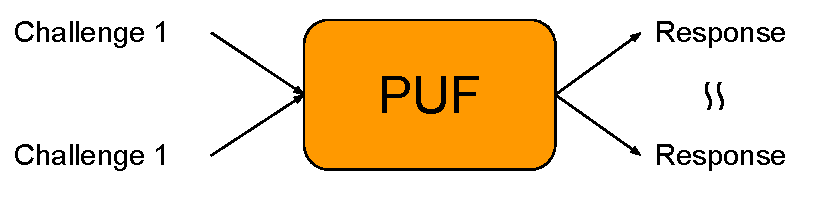
\includegraphics[width=0.75\textwidth]{images/reproducibility}
    \caption[reproducibility: responses to the same PUF challenge need to be similar]{reproducibility: responses to the same PUF challenge need to be similar~\cite{Kodytek2017}}
    \label{fig:reproducibility}
\end{figure}

\subsection*{Uniqueness}

While reproducibility talks about the behaviour of a specific \gls{puf}, uniqueness is defined with respect to a set of different \gls{puf} instances. Given the same challenge, two \glspl{puf} must produce a response that is different enough in the given metric. The metric used is the inter-Hamming distance (which will be defined later in Section~\ref{sec:uniqueness}).

\begin{figure}[ht!]
    \centering
    \captionsetup{justification=centering,margin=0.5cm}
    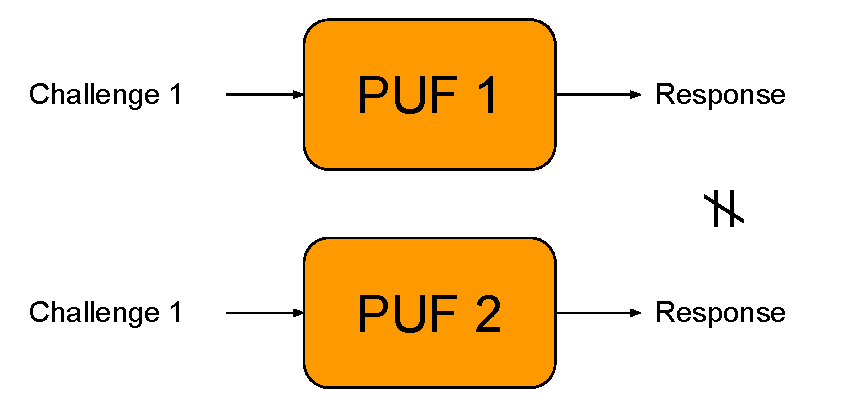
\includegraphics[width=0.75\textwidth]{images/uniqueness}
    \caption[uniqueness: two PUF instances must produce different responses if given the same challenge]{uniqueness: two PUF instances must produce different responses if given the same challenge~\cite{Kodytek2017}}
    \label{fig:uniqueness}
    % TODO cite
\end{figure}

\subsection*{Identifiability}\label{sec:identifiability}

Identifiability is tied to both uniqueness and reproducibility. Given a single challenge, if the responses from the same \gls{puf} are similar and responses from different \glspl{puf} are different enough, the responses can be used as a means of identification of each \gls{puf}. More formal characterization of the words `similar' and `different' as well as a concrete protocol for \gls{puf} identification is explained in Sections~\ref{sec:puf_evaluation} and~\ref{sec:identification}.

\subsection*{Physical unclonability}
 
Physical unclonability enforces that it is hard to break the uniqueness property. The `hardness' is expressed as a technical and physical infeasibility of creating two nearly identical \gls{puf} instances. In practice, even the manufacturer is unable to break uniqueness due to the uncontrollable physical laws on which the \gls{puf} implementation relies.

\subsection*{Unpredictability}

A \gls{puf} is said to be unpredictable, if given a limited set of challenge-response pairs, it is impossible to create an algorithm that predicts the remaining responses based on a challenge. This means that the challenge-response pair space is sufficiently random.

\subsection*{Mathematical unclonability}

While physical unclonability talks about the impossibility of creating a real-world clone of a specific \gls{puf}, mathematical unclonability requires that no algorithm can predict the \gls{puf} behaviour.

Mathematical unclonability is a stronger model of unpredictability. It assumes unlimited physical access to a specific \gls{puf} instance. The potential adversary can learn as many challenge-response pairs as he is capable of storing and can potentially make use of other \gls{puf} observations. Even in this situation, it should be impossible for the adversary to create a prediction algorithm capable of outputting a response based on a given challenge. 

Mathematical unclonability implies that the specific \gls{puf} implementation has a large number of possible challenges (more than the adversary could theoretically store). If this was not true, a simple lookup table of challenge-response pairs could be constructed, breaking mathematical unclonability. % TODO mention strong PUFs?

\subsection*{True unclonability}

\gls{puf} is considered truly unclonable if it is physically and mathematically unclonable. True unclonability thus implies mathematical and physical unclonability.

\subsection*{One-Wayness}

The one-wayness property is similar to the requirement of cryptographic one-way functions (for example hash functions). Given a \gls{puf} instance and a response, it should be impossible to create an inversion algorithm that can find a corresponding challenge to the response.

Similar to mathematical unclonability, the \gls{puf} needs to have a sufficiently large set of possible challenges and resulting responses in order to meet this property. Otherwise, it would be possible to construct a complete lookup table and find the wanted challenge.

\begin{figure}[h!]
    \centering
    \captionsetup{justification=centering,margin=0.5cm}
    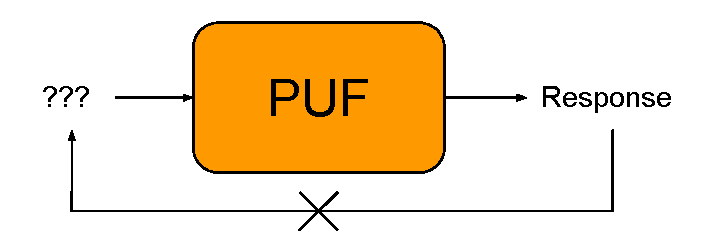
\includegraphics[width=0.75\textwidth]{images/one-wayness}
    \caption{one-wayness: it is impossible to find a challenge corresponding to a given response}
    \label{fig:one-wayness}
\end{figure}

\subsection*{Tamper Evidence}

Tampering with devices in order to compromise their integrity has proven to be a successful technique. For example, invasive attacks (such as microprobing) are able to extract sensitive data from the target system.\cite{Kommerling1999}

Tamper evidence helps to mitigate such attack vectors. The \gls{puf} must detect the attempt to tamper with the system and change its challenge-response pairs to a different set as if the \gls{puf} instance transforms itself to a completely different one.

To achieve this property, the \gls{puf} implementation needs to rely on physical properties that will necessarily change if the device is tampered with. This change will inherently transform the \gls{puf}.

%--------------------------------
\section{PUF classification}
%--------------------------------

A lot of different \gls{puf} implementations have been proposed. They can be classified based on fabrication, security and intrinsic evaluation\cite{Shital2017}\cite{McGrath2019}. A diagram of the discussed \gls{puf} classes is depicted in figure~\ref{fig:classification}.

\begin{figure}[ht!]
    \centering
    \captionsetup{justification=centering,margin=0.5cm}
    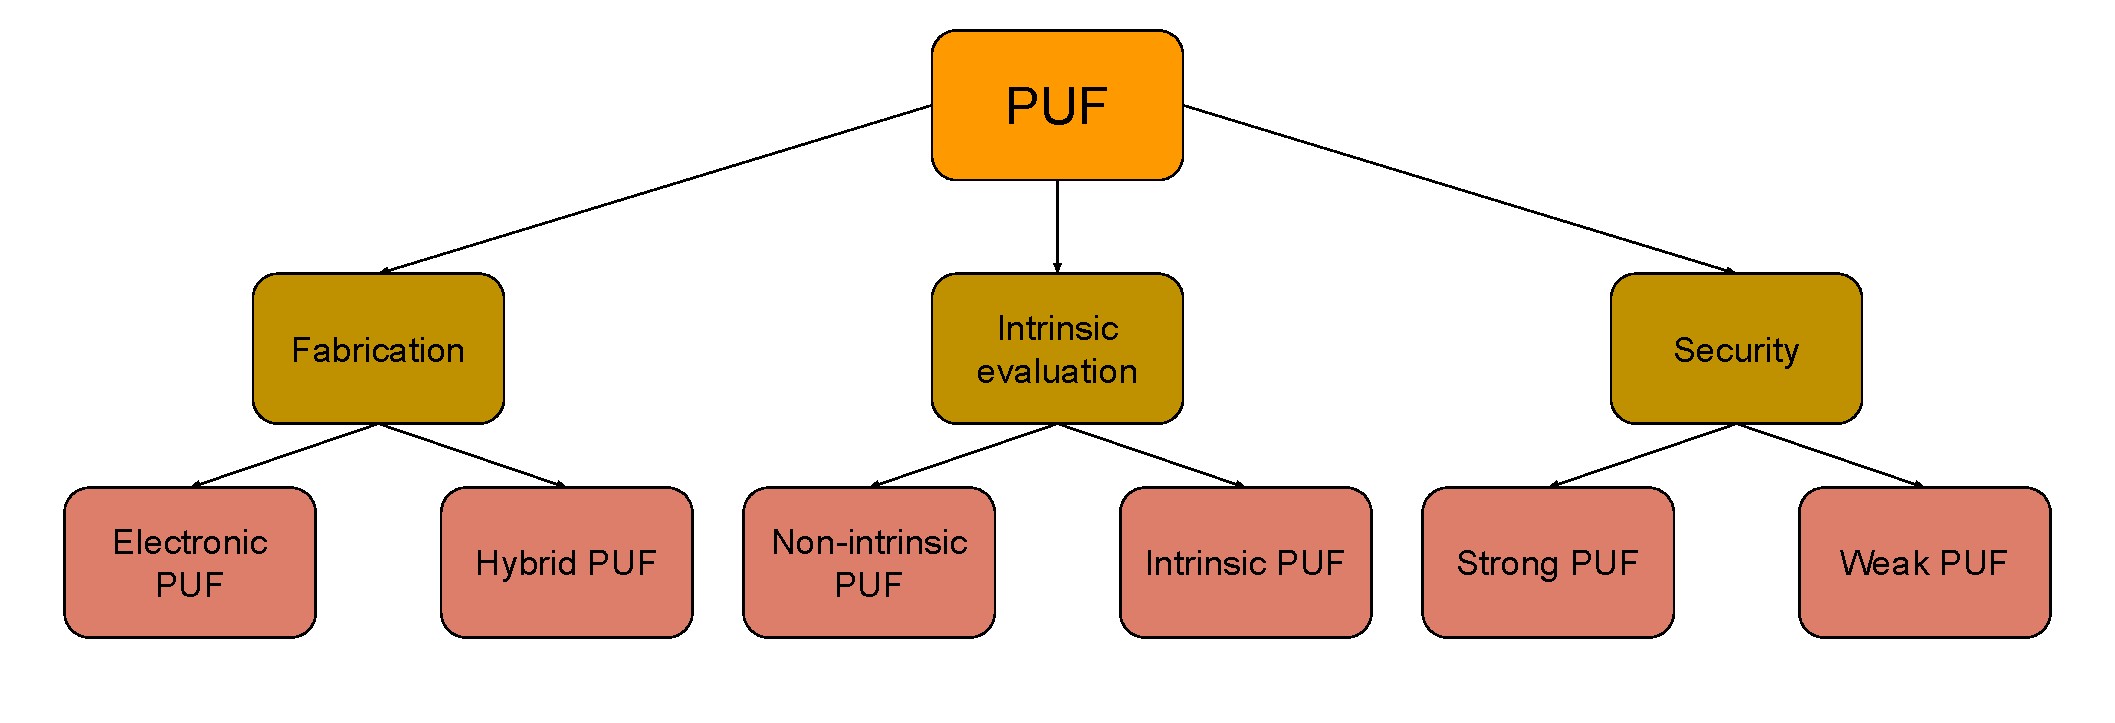
\includegraphics[width=\textwidth]{images/classification}
    \caption{classification of PUFs}
    \label{fig:classification}
\end{figure}

\subsection{Electronic, silicon and hybrid PUFs}

Electronic \glspl{puf} source their randomness from electronic components. This means that they rely on properties such as capacitance, resistance or propagation delay of a circuit.

A large subclass of electronic \glspl{puf} is silicon \glspl{puf}. They can be constructed only using \gls{cmos} technology, therefore they can be implemented on the same die together with the main chip. This prevents the need to interface with additional circuitry using external buses, lowering cost and limiting the possibility of leaking sensitive data.\cite{Maes2013}

Examples of electronic \glspl{puf} are \gls{sram} \gls{puf}, \gls{ropuf} or arbiter \gls{puf}.

Hybrid \glspl{puf} use non-electronic phenomena to create their challenge-response pairs. While randomness introduced into the system is of non-electronic nature, the signal is usually processed and stored using electronic components. Hence the name hybrid \glspl{puf}. They can be based on optics (optical \gls{puf}), magnetism (magnetic \gls{puf}) or quantum effects (quantum \gls{puf}\cite{Koustubh2021}).


\subsection{Intrinsic and non-intrinsic PUFs}

A \gls{puf} implementation is said to be intrinsic if it satisfies the following two conditions:

\begin{enumerate}
    \item responses are evaluated internally
    \item instance-specific random features are introduced implicitly during the manufacturing process
\end{enumerate}

Internal evaluation requires the measurement equipment of the \gls{puf} to be embedded in the device. This, similar to silicon \glspl{puf}, lowers cost and is more secure.

The second condition discusses the introduction of randomness into the system. Implicit randomness relies on process variations taking place during normal manufacturing, while explicit randomness needs to be created by special procedures which would have not been needed otherwise (such as doping with random dielectric particles for the construction of a coating \gls{puf}\cite{Kori2006}).

\gls{sram} and arbiter \glspl{puf} are examples of intrinsic \glspl{puf}. If the \gls{puf} construction does not satisfy the given properties, it is called non-intrinsic. For example, optical or coating \glspl{puf} are non-intrinsic.\cite{Maes2012}

\subsection{Strong and weak PUFs}

Security based classification distinguishes \gls{puf} implementations according to the size of their challenge-response pair sets.

In order for a \gls{puf} to be classified as strong, its challenge-response pair set needs to be sufficiently large to prevent an exhaustive search by a possible attacker. The challenge-response pair size thus scales well (preferably exponentially) with some construction parameter.\cite{Guajardo2007}

On the other hand, weak \glspl{puf} have only a limited set of challenge-response pairs. Some \glspl{puf} can only have one pair. They are sometimes called \gls{pok}.

As the naming implies, strong \gls{puf} constructions possess, in some sense, greater security. Weak \glspl{puf} cannot be mathematically unclonable (and consequently cannot be truly unclonable or unpredictable). Strong \glspl{puf} can also be used in more applications, as explained in Section~\ref{sec:puf_applications}. However, it turns out that constructing a strong \gls{puf} is a very hard problem.\cite{Maes2013}

%--------------------------------
\section{PUF evaluation parameters}\label{sec:puf_evaluation}
%--------------------------------

As \glspl{puf} rely on uncontrollable physical processes to produce their responses, it is crucial to perform an analysis of their quality. Several evaluation parameters were defined by~\cite{Mispan2018},~\cite{Leest2010} and~\cite{Maiti2011} and they will be discussed here.

These parameters enable us to quantify the performance of \glspl{puf} and compare them. Some of them will be used to evaluate the \gls{sram} \gls{puf} implemented in this thesis in Sections~\ref{sec:rtc_evaluation} and~\ref{sec:deepsleep_evaluation}.

\noindent\newline
The following evaluation parameters will be defined:
\begin{itemize}
    \item Uniformity
    \item Reliability
    \item Uniqueness
    \item Bit-aliasing
    \item Randomness
\end{itemize}

Before the parameters can be defined, a notation used in the upcoming text is described here and in Table~\ref{table:notation} to avoid possible confusion.

The Hamming weight $\textrm{HW}(x)$ of a bit string \emph{x} is defined as the number of one bits in the string. 

The Hamming distance $\textrm{HD}(x, y)$ of two bit strings \emph{x} and \emph{y} is defined as a number of positions where the bits of \emph{x} and \emph{y} differ.

The reference response $R_{i}^{'}(n)$ is the expected response of \emph{n} bits produced by the chip \emph{i}. It is usually computed as a bitwise average between \emph{m} response samples taken in normal operating conditions. However, some works choose the reference response as the first measured sample.\cite{Kodytek2020}

\begin{table}[h!]
\centering
\begin{tabular}{c l} 
     Notation & Description\\
     \hline
     k & The number of devices\\ 
     m & The number of response samples\\
     n & The number of bits in a response\\ 
     $R_{i,j}(n)$ & The \emph{j}-th response (containing \emph{n} bits) of \emph{i}-th chip\\ 
     $R_{i}^{'}(n)$ & The reference response of \emph{i}-th chip, containing \emph{n} bits\\ 
     $r_{i,j}^{'}$ & The \emph{j}-th bit of a reference response of chip \emph{i}\\
     $\textrm{HW}(x)$ & The Hamming weight of \emph{x}\\
     $\textrm{HD}(x, y)$ & The Hamming distance between \emph{x} and \emph{y}\\
     \hline
    \end{tabular}
    \captionsetup{justification=centering,margin=0.5cm}
    \caption{Notation used in evaluation parameters definitions}
    \label{table:notation}
\end{table}

\subsection{Uniformity}\label{sec:uniformity}

Uniformity represents a proportion of zero and one states of the response bits. It is useful to determine if there exists a global bias towards any of these states. Since the \gls{puf} responses need to be unpredictable, there should not be any bias. Thus, the ideal value of uniformity is 50\%.

The uniformity property for one response of chip \emph{i} is defined by Equation~\ref{eq:uniformity}:

\begin{equation}\label{eq:uniformity}
    U_{i} = \frac{1}{n}\sum_{j=1}^{n}r_{i,j}^{'} = \frac{\textrm{HW}(R_{i}^{'}(n))}{n} \cdot 100\% 
\end{equation}

Uniformity can also be calculated as an average value between k \gls{puf} instances of the same type by Equation~\ref{eq:avg_uniformity}\cite{Maiti2011}:

\begin{equation}\label{eq:avg_uniformity}
    U_{\textrm{avg}} = \frac{1}{k}\sum_{i=1}^{k}U_{i} = \frac{1}{k}\sum_{i=1}^{k}\frac{\textrm{HW}(R_{i}^{'}(n))}{n} \cdot 100\%
\end{equation}

Since uniformity only measures a global proportion of the response bit states, it is not a perfect tool to detect a possible local bias. A trivial example could be a response defined in the following way:

\begin{equation}
    r_{i, j}^{'} =
    \begin{cases*}
        1 & if $j < \frac{m}{2}$ \\
        0 & otherwise
    \end{cases*}
\end{equation}

That is the first half of the response bits are ones and the second half are all zero bits. Uniformity $U_{i}$ for such a response is close to the ideal value of $50\%$ though the response is clearly not unpredictable.

\subsection{Reliability}\label{sec:reliability}

Reliability is a parameter that measures the consistency of \gls{puf} responses to the same challenge. It is tied to the reproducibility property from Section~\ref{sec:reproducibility}.

In order to calculate reliability, the intra-Hamming distance for a chip \emph{i} needs to be defined first\cite{Maiti2011}: 

\begin{equation}\label{eq:hd_intra}
    \textrm{HD-intra}_{i} = \frac{1}{m} \sum_{j=1}^{m}\frac{\textrm{HD}(R_{i,j}(n), R_{i}^{'}(n))}{n} \cdot 100 \%
\end{equation}

The reference $R_{i}^{'}(n)$ is obtained at nominal operating conditions (room temperature and normal voltage). The responses $R_{i, j}(n)$ are then taken at different conditions and the result is calculated. It essentially represents the percentage of bits that change compared to the reference response.

Reliability is then defined by Equation~\ref{eq:reliability}:

\begin{equation}\label{eq:reliability}
    \textrm{Reliability} = 100\% - \textrm{HD-intra}
\end{equation}

Since the reproducibility property requires \glspl{puf} to produce similar responses to the same challenge, the ideal $\textrm{HD-intra}_{i}$ value is $0\%$ and thus reliability needs to be close to $100\%$.

\subsection{Uniqueness}\label{sec:uniqueness}

Uniqueness measures how much responses from different \glspl{puf} vary. It is estimated by the inter-Hamming distance defined by Equation~\ref{eq:uniqueness}:

\begin{equation}\label{eq:uniqueness}
    \textrm{HD-inter} = \frac{2}{k(k-1)}\sum_{i=i}^{k-1} \sum_{j=i+1}^{k} \frac{\textrm{HD}(R_{i}^{'}(n),R_{j}^{'}(n))}{n} \cdot 100\%
\end{equation}

The original definition of $\textrm{HD-inter}$ by~\cite{Maiti2010} does not specify how to choose the responses to calculate the Hamming distance from. However,~\cite{Kodytek2020} uses the reference responses and this definition will be used in future calculations in this thesis.

The inter-Hamming distance takes all combinations of pairs of devices and computes the average Hamming distance of their responses. The uniqueness property of \glspl{puf} in Section~\ref{sec:properties} requires that the responses should differ as much as possible. This is achieved when $\textrm{HD-inter}$ is close to its ideal value of $50\%$.

\subsection{Bit-aliasing}\label{sec:bit_aliasing}

Uniformity in Section~\ref{sec:uniformity} looks at the global bias of \gls{puf} responses from a single device. On the other hand, bit-aliasing measures the proportion of zero and one state of a single bit across different devices.

Bit-aliasing is calculated as the percentage Hamming weight of the \emph{j}-th bit. It is defined by Equation~\ref{eq:bit_aliasing}\cite{Maiti2011}:

\begin{equation}\label{eq:bit_aliasing}
    \textrm{Bit-aliasing}_{j} = \frac{1}{k}\sum_{i=1}^{k}r_{i, j}^{'} \cdot 100\%
\end{equation}

Same as for uniformity, the ideal value for bit-aliasing is $50\%$. Values close to 0 or 100\% would indicate bits that stay the same across different \gls{puf} instances, violating the uniqueness property.

\subsection{Randomness}

As \gls{puf} responses need to be unpredictable, they are required to contain sufficient entropy. According to~\cite{Leest2010}, there are several ways to test whether the response data is sufficiently random. Two are described here, the compression test and the \acrshort{nist} randomness test.

\subsubsection*{NIST randomness test}

The \acrshort{nist} randomness test uses the \acrshort{nist} statistical test suite to determine if the data is sufficiently random. Each test from the battery is tested for the null hypothesis that the response data is truly random on some set significance level.

Furthermore, each test is executed multiple times on different sequences of the data and a p-value for each run is calculated. These p-values are then tested for the null hypothesis that they are from a uniform distribution, as would be the case for truly random data.\cite{NIST2010}

However, not all tests can be used as they require more input data than is practically possible to generate by the \gls{puf}. Tests for which only 170-bit string suffices are listed here\cite{Leest2010}:

\begin{itemize}
    \item Frequency (monobit) test
    \item Frequency test within a block
    \item Runs test
    \item Test for longest run of ones in block
    \item Serial test
    \item Approximate entropy test
    \item Cumulative sums (Cusum) test
\end{itemize}

\subsubsection*{Compression test}

The idea behind compression test is simple. If a lossless compression algorithm is able to reduce the size of the tested data, it does not have full entropy\footnote{Meaning the entropy in bits is the same as the length of the data in bits.}\cite{Leest2010}.

A good example of a compression algorithm to use is the \gls{ctw} algorithm as it was shown to produce the best results out of the commonly used entropy estimators\cite{Yun2008}.

\section{PUF applications}\label{sec:puf_applications}
%--------------------------------

Thanks to the properties described in Section~\ref{sec:properties}, \glspl{puf} are suitable for several cryptographic applications. Three main uses of \glspl{puf} according to~\cite{Maes2012} will be described here: identification, authentication and cryptographic key generation.


\subsection{Identification}\label{sec:identification}

A \gls{puf} can be compared to a device's fingerprint. The \gls{puf} provides an inherent identifying feature\footnote{Inherent identity is a unique characteristic of the device itself (a \gls{puf} response), while assigned identity is an artificially made up property (a serial number).} to the entity encapsulating it.  Therefore, device identification is a natural application for \glspl{puf}. A simple identification protocol using the device's \gls{puf} is described.

The process of device identification consist of two phases: enrollment and identification\cite{Maes2012}.

\begin{description}
    \item[Enrollment phase:] \hfill \\ In this phase, the inherent identifying feature of every considered device is collected. This means saving a \gls{puf} response from each device to a database.
    \item[Identification phase:] \hfill \\ When the device needs to be identified, it generates its \gls{puf} response. The response is then compared to other responses stored in the database.
\end{description}

However, the comparison of the presented \gls{puf} response is not straightforward. Since the \gls{puf} relies on physical state of the system, errors can arise while generating responses. For this reason, comparison is based on the \gls{hd} rather than on equality.

The property of identifiability (discussed in Section~\ref{sec:identifiability}) tells us that responses from a specific device will be similar (have low \gls{hd}) and responses from different devices will be far apart (have high \gls{hd}). Thus, a threshold value of \gls{hd} needs to be chosen. Responses with lower \gls{hd} than the threshold will be considered to have originated from the same device.

\begin{figure}[ht!]
    \centering
    \captionsetup{justification=centering,margin=0.5cm}
    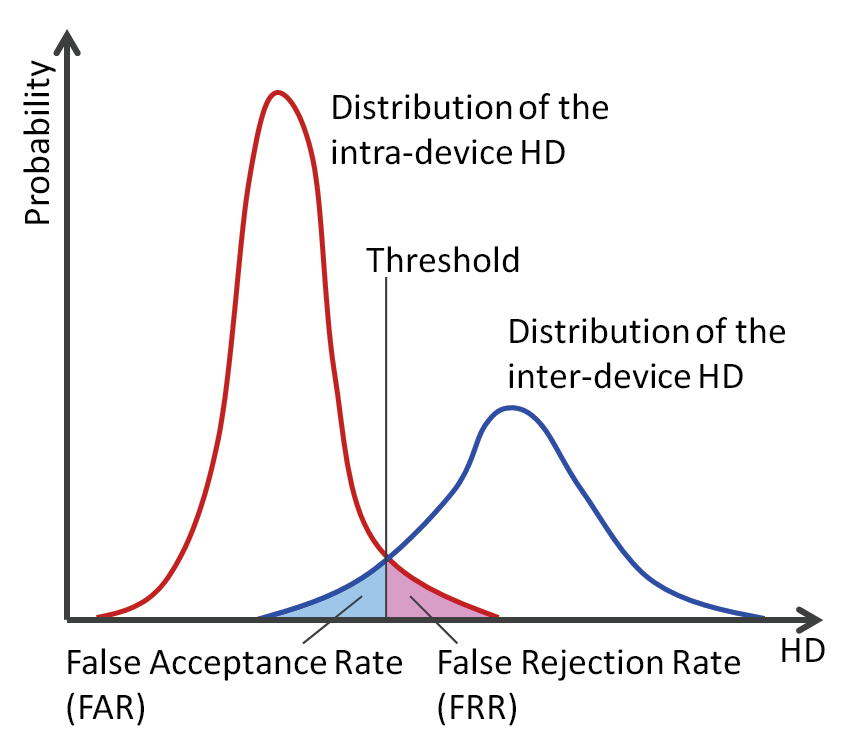
\includegraphics[scale=0.25]{images/identification_histogram.png}
    \caption[PUF identification: intra and inter HD distributions]{PUF identification: intra and inter HD distributions\cite{Hori2013}}
    \label{fig:puf_inter_intra_hd}
\end{figure}

The threshold can be chosen based on the distributions of inter and intra \glspl{hd}. While the inter-\gls{hd} is a measure of how responses from different devices differ, the intra-\gls{hd} indicates the similarity of responses from the same device.

If the distributions of inter and intra \glspl{hd} do not overlap, threshold value between the distributions is optimal. The \gls{far} (a probability of falsely identifying a device) and \gls{frr} (the probability of falsely rejecting a device) are zero.

If the distributions overlap, a compromise between \gls{far} and \gls{frr} must be made. Reducing \gls{far} will inevitably increase \gls{frr} and vice versa. Figure~\ref{fig:puf_inter_intra_hd} illustrates a possible intra and inter \gls{hd} distributions and a chosen threshold.

\subsection{Authentication}

Authentication requires the entity, which wants to authenticate itself to a verifier, to provide a proof of its identity. The entity also needs to convince the verifier that it actively participated in the creation of the proof.\cite{Maes2012}

A simple protocol based on the challenge-response pairs of \glspl{puf} will be presented here. It is divided into two distinct phases: enrollment and authentication.\cite{Devadas2008}

\begin{description}
    \item[Enrollment phase:] \hfill \\ During this phase, a trusted third party (the verifier) is in possession of the device which will later be authenticated. A sufficient number of randomly generated challenges along with the corresponding responses (obtained from the device) is saved to a database.
    \item[Authentication phase:] \hfill \\ When the device needs to be authenticated, the verifier chooses a challenge from the database and sends it to the device. The device then responds with the corresponding response. Finally, the obtained and the previously recorded responses are compared. If they are sufficiently similar, the device is authenticated successfully. This challenge-response pair is then deleted from the database and never used again.
\end{description}

The whole process of this \gls{puf}-based authentication protocol is illustrated in Figure~\ref{fig:authentication_process}.

\begin{figure}[ht!]
    \centering
    \captionsetup{justification=centering,margin=0.5cm}
    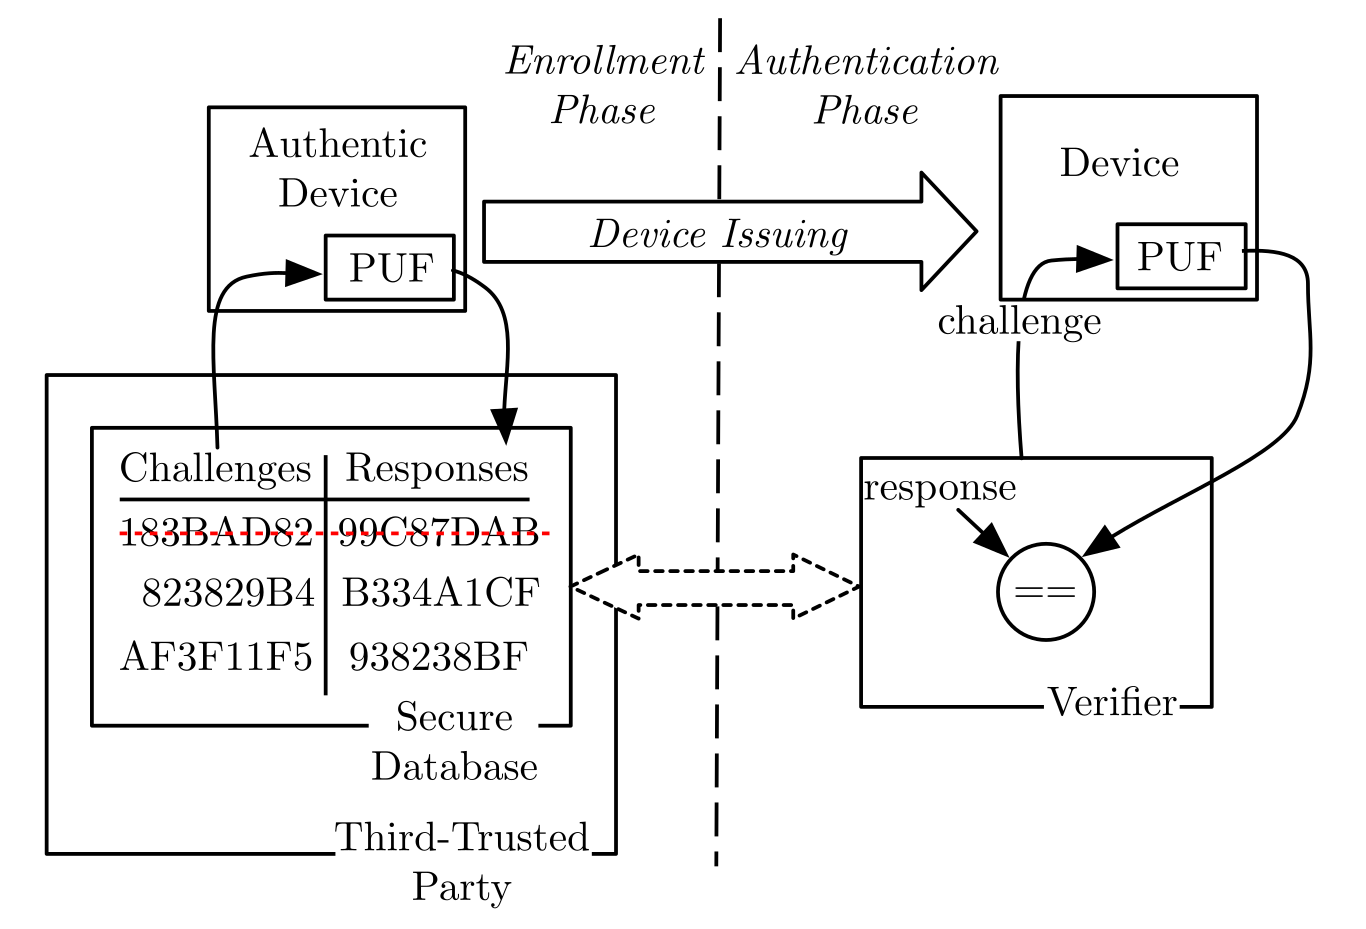
\includegraphics[width=0.7\textwidth]{images/authentication_process.png}
    \caption[PUF-based authentication protocol]{PUF-based authentication protocol\cite{Barbareschi2018}}
    \label{fig:authentication_process}
\end{figure}

The comparison of the responses is done in the same way as in \gls{puf}-based identification (Section~\ref{sec:identification}). The \gls{hd} is used as a distance metric and a threshold for accepting the response must be chosen appropriately.

The challenge-response pairs are deleted from the database and never reused to prevent a potential man-in-the-middle attack. Since this is not a threat, the communication between the device and the verifier does not need to be secured.

This protocol is simple and has its drawbacks. It only provides a limited number of authentications for the verifier given by the number of stored challenge-response pairs. The authentication is only one-way, the verifier is never authenticated to the device. It requires the \gls{puf} to be strong (to have a large number of available challenge-response pairs).

More advanced \gls{puf}-based authentication protocols that address some of the aforementioned drawbacks have been developed by~\cite{Maes2013},~\cite{Barbareschi2018} and~\cite{Rostami2014}.

\subsection{Key generation}

Keys are required in the majority of cryptographic applications. They need to contain true randomness in order to be unpredictable and unique. The cryptographic key then needs to be stored and retrieved securely. These conditions are hard to meet and a myriad of cryptographic systems have been broken because of bad generation or handling of keys.\cite{Maes2012_2}

\gls{puf}-based cryptographic key generation tries to solve those problems. The key is not stored in any memory and is generated by the \gls{puf} on demand. In some way, it is imprinted in the \gls{puf} itself. Furthermore, the uniqueness and unpredictability property of \glspl{puf}, which arise from their uncontrollable physical properties, introduce the necessary randomness.

Since the \gls{puf} responses are noisy and not 100\% reliable, care needs to be taken while generating cryptographic keys. The keys need to be the same every time, otherwise the cryptographic algorithms using it would not produce the desired output. For this reason, \glspl{ecc} are used to obtain the same key every time with sufficient probability.

\begin{figure}[h!]
    \centering
    \captionsetup{justification=centering,margin=0.5cm}
    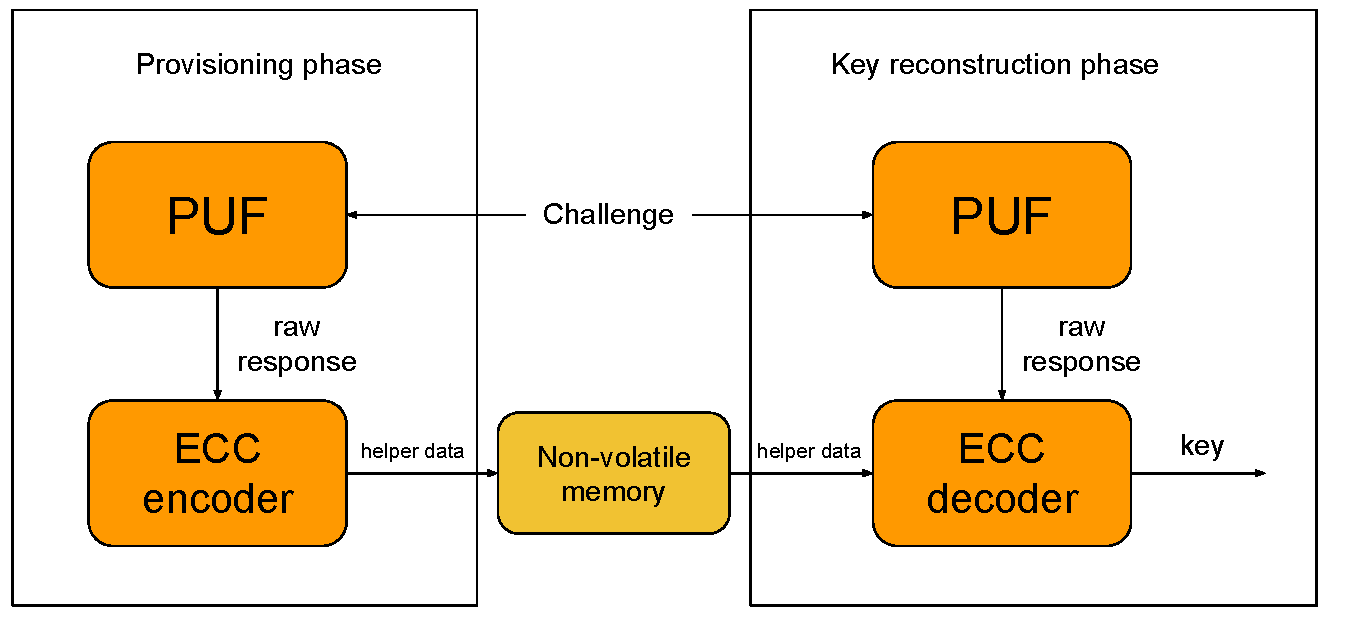
\includegraphics[width=\textwidth]{images/key_generation.pdf}
    \caption[PUF-based key-generation mechanism]{PUF-based key-generation mechanism, inspired by~\cite{Gao2017}}
    \label{fig:key_generation}
\end{figure}

The process of \gls{puf}-based key generation is divided into two phases: enrollment and key reconstruction\cite{Mispan2018}. It is illustrated in Figure~\ref{fig:key_generation}.

\begin{description}
    \item[Enrollment phase:] \hfill \\ In this phase, \gls{puf} responses are generated and processed by the \gls{ecc} algorithm to construct the cryptographic key. The \gls{ecc} calculates helper data from the key and saves it to a non-volatile memory. This data will later be used to reconstruct the key. The helper data can also contain a \gls{puf} configuration.
    \item[Key regeneration phase:] \hfill \\ When the key is needed, the \gls{puf} produces a response and feeds it to the \gls{ecc} algorithm. The key is then reconstructed by the \gls{ecc} using the response and the corresponding helper data saved in the non-volatile memory.
\end{description}

The \gls{ecc} used is usually a simple repetition code or a \gls{bch} code. However, any \gls{ecc} can be used and the codes can even be concatenated in order to increase efficiency.\cite{Bosch2008}

After key regeneration, a raw bit string key is obtained. It can be used immediately with some cryptosystems (typically symmetric ciphers such as AES). However, some systems put restrictions on the key (RSA needs two prime numbers), thus requiring further processing. % TODO kde jsem ztratil zdroj?

Key generation is a typical application of weak \glspl{puf}\cite{Herder2014}. As the \gls{sram} \gls{puf} implemented in this thesis is classified as weak, a simple key generation algorithm will be tested on top of the \gls{puf}.

It is even possible for a weak \gls{puf} to provide authentication without the need for a large number challenge-response pairs. Once the key is generated by the weak \gls{puf}, it can be used in other cryptographic algorithms which provide authentication such as \gls{mac} or digital signatures (at the cost of additional hardware/software).\cite{Herder2014}


% TODO hash po rekonstrukci klice? (zdroj FPGA Intrinsic PUFs and Their Use for IP Protection jako privacy amplification)

%--------------------------------
\section{PUF implementations}
%--------------------------------

\subsection{Optical PUF}\label{sec:optical_puf}
\subsection{SRAM PUF}
\subsubsection*{SRAM PUF and its properties}\label{sec:srampuf_properties}
% TODO mozna neco o SRAM aging? (intrinsicID meli nejaky whitepaper)


\chapter{SRAM PUF}\label{sec:sram_puf}

\gls{sram} \gls{puf} is based on a random startup behaviour of individual \gls{sram} cells. It was first proposed by~\cite{Guajardo2007} in 2007.

In a \gls{cmos} implementation (which is used to create 99\% of integrated circuits as of 2011~\cite{Voinigescu2013}) a \gls{sram} cell is usually made up of two cross-coupled inverters. The inverters reinforce each other of their state, thus creating a bistable circuit---a circuit with only two stable states. This enables the cell to save exactly one logical bit. Each inverter is implemented using two transistors and additional two transistors are used to enable read and write operations. This means that storage of a single bit costs six transistors in hardware.~\cite{Maes2010}

The logical diagram of a \gls{sram} cell containing the two inverters is illustrated in Figure~\ref{fig:sram_cell_logic} and a diagram with the transistor layout of the cell is shown in Figure~\ref{fig:sram_cell_cmos}.

\begin{figure}[h!]
    \centering
    \captionsetup{justification=centering,margin=0.5cm}
    \begin{subfigure}[c]{0.5\textwidth}
        \centering
        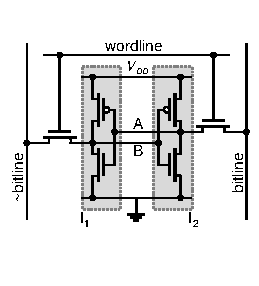
\includegraphics[width=0.85\linewidth]{images/transistor_sram_cell.pdf}
        \caption{A CMOS diagram of a SRAM cell}
        \label{fig:sram_cell_cmos}
    \end{subfigure}%
    \begin{subfigure}[c]{0.5\textwidth}
        \centering
        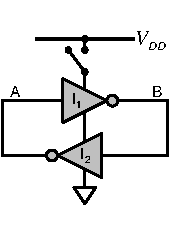
\includegraphics[width=0.6728\linewidth]{images/logic_sram_cell.pdf}
        \caption{A logic circuit diagram of a SRAM cell}
        \label{fig:sram_cell_logic}
    \end{subfigure}
    \caption[CMOS and logic circuit diagrams of a SRAM cell]{CMOS and logic circuit diagrams of a SRAM cell~\cite{Maes2012}}
    \label{fig:sram_cell}
\end{figure}

The principle of a \gls{sram} \gls{puf} is based on the power-up values of the memory cells. The memory cells are volatile---when power is lost, the data disappears from memory. After startup, each cell has to initialize to either a `1' or a `0' state. Which state the cell stabilizes on is dependent on a relative strength\footnote{Strength here means the properties of the underlying \gls{mosfet} transistors (such as delay).} of the two inverters. Since the inverters are designed identically, their strength is determined by random process variations during manufacturing.~\cite{Maes2010}

For each cell independently, the two following cases can happen:

\begin{enumerate}
    \item One of the inverters has far greater strength than the other. The cell has a significant preference for one initial state. Meaning it will either be in the `0' or the `1' state most of the time after power-up. This case is crucial for the \gls{puf} construction.
    \item By chance, strengths of the two inverters are nearly identical. The resulting initial state depends on random noise in the circuit. This is the source of unreliability of the \gls{puf}.
\end{enumerate}

During fabrication, each cell acquires its specific properties and thus its startup state stability according to the cases mentioned above. However, stability is not a discrete property. One cell can be less stable than some other. An illustration of this can be seen in Figure~\ref{fig:sram_puf_stability}.

\begin{figure}[ht!]
    \centering
    \captionsetup{justification=justified,margin=0.5cm}
    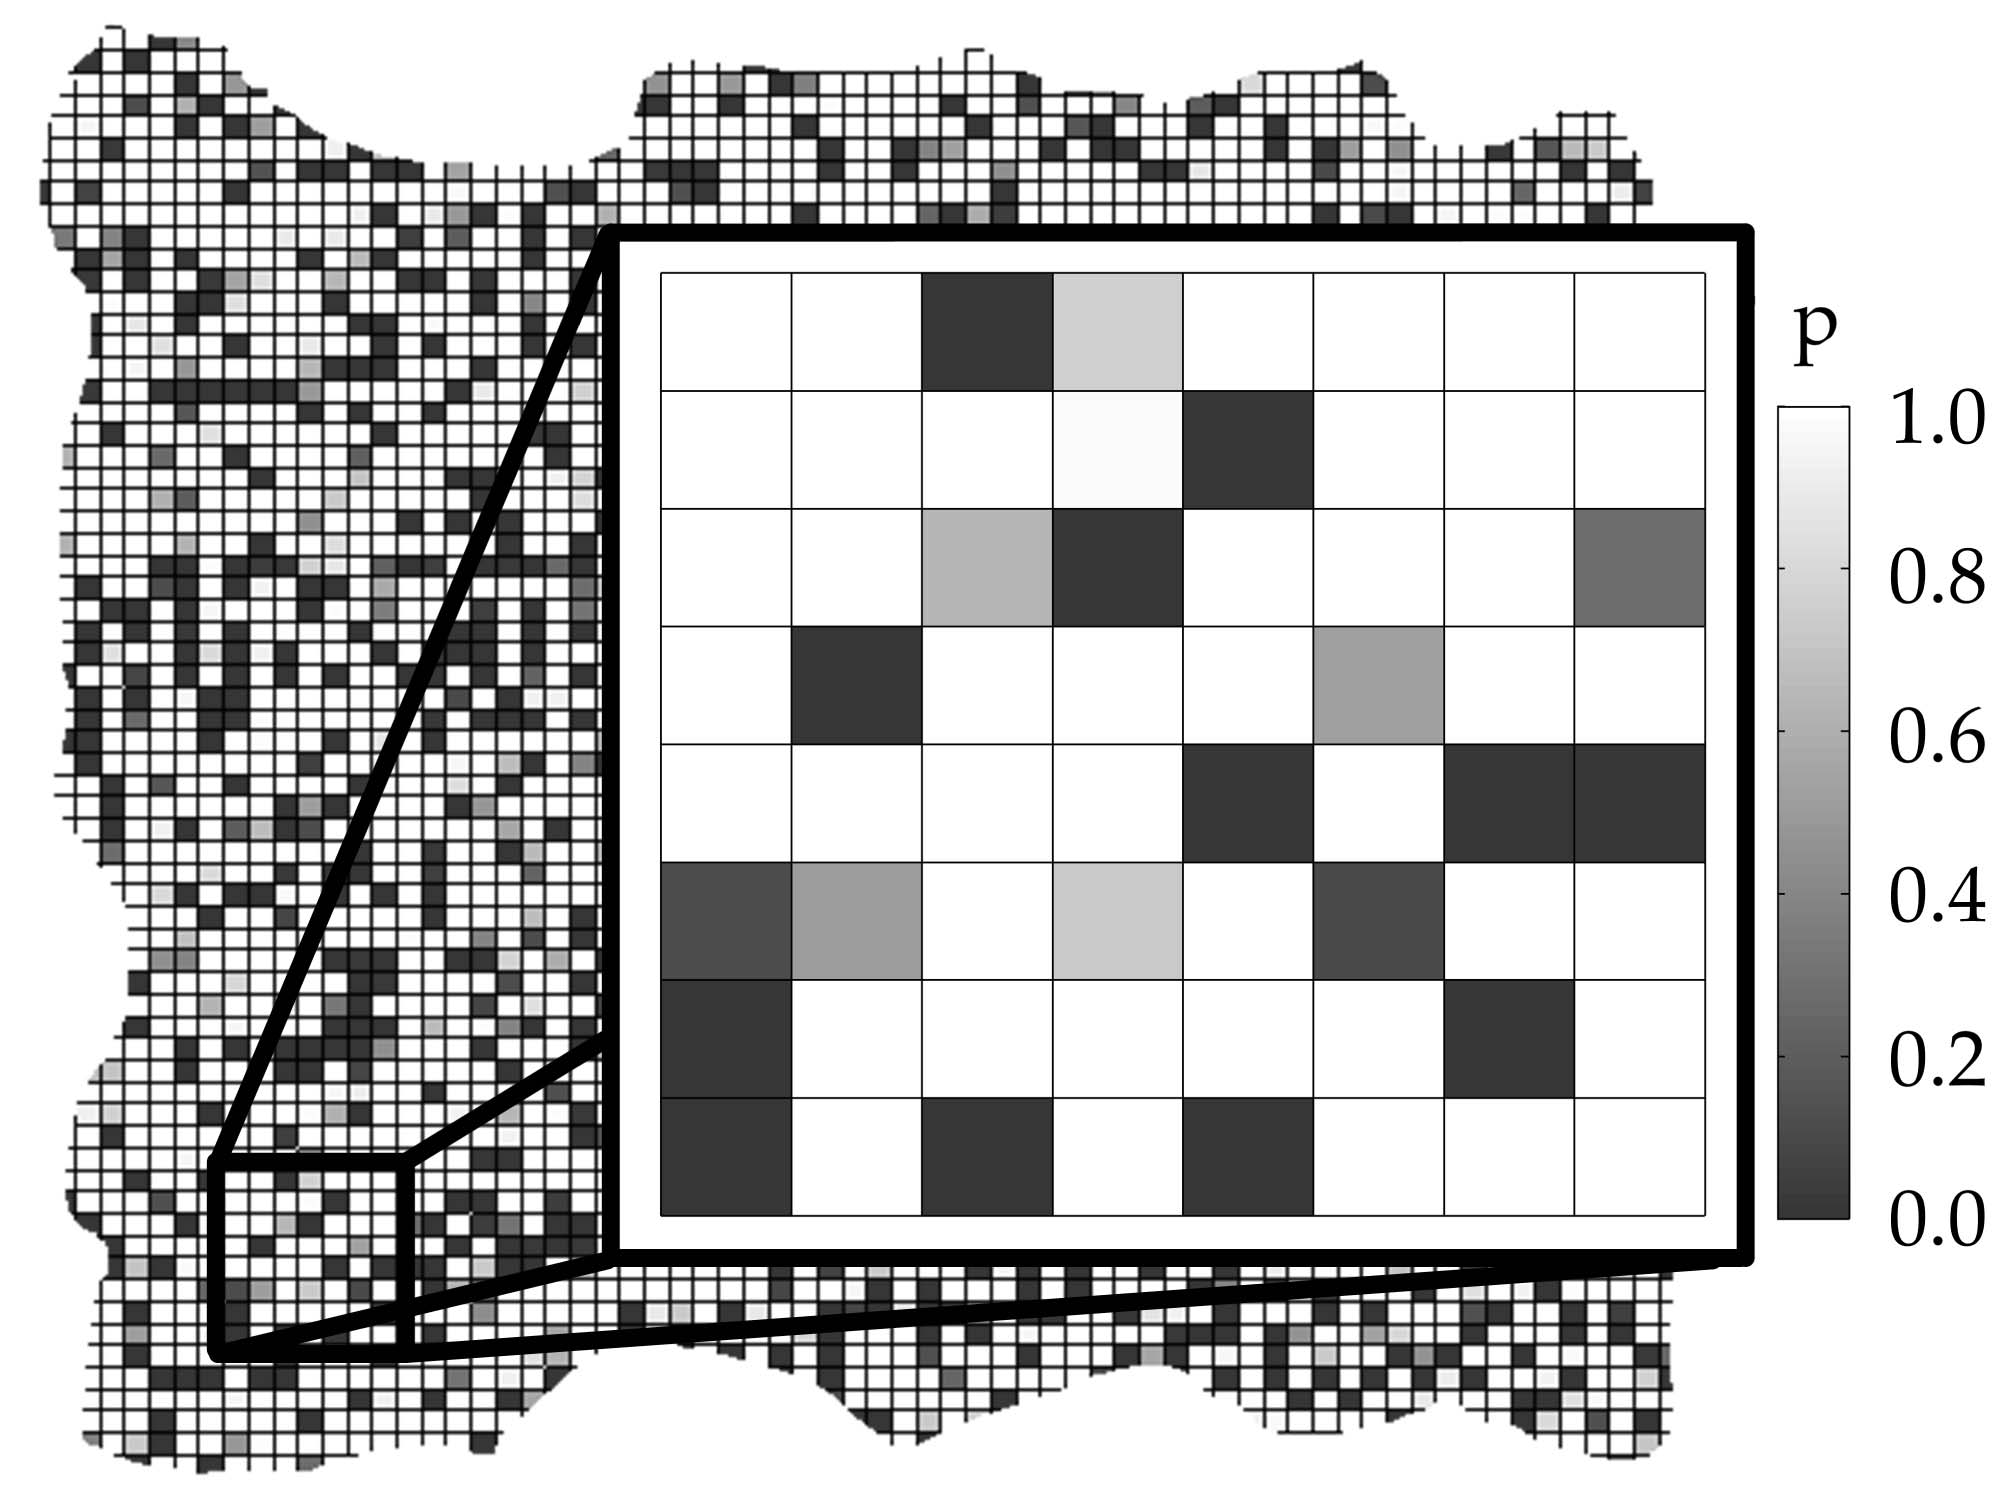
\includegraphics[width=0.5\textwidth]{images/sram_puf_stability.jpg}
    \caption[Illustration of SRAM cell stability.]{Illustration of SRAM cell stability. A small area of SRAM cells is shown. The lightness of each cell indicates the probability that the cell's startup state will be `1'. Note that most of the cells are either nearly black or nearly white. Meaning they are stable and their preferred state is `0` or `1` respectively.~\cite{Holcomb2009}}
    \label{fig:sram_puf_stability}
\end{figure}

It turns out, that the process variations are significant enough that most \gls{sram} cells tend to be stable. This enables the startup values of memory to be used as \gls{puf} responses. Challenge can be interpreted as a concrete address in memory. The response is then read from this address.~\cite{Maes2013}

For the construction of a \gls{sram} \gls{puf}, stable cells are important. The unstable ones can be considered harmful as they decrease reliability. However, thanks to their unknown initial state which is determined randomly after every startup, they are useful for the construction of \glspl{trng}.~\cite{Holcomb2009}

A huge advantage of \gls{sram} \glspl{puf} is, that \gls{sram} memory is usually already present in chips. If the device possesses a suitable mechanism of power state control of its memory (the ability to turn off blocks of memory, power-saving states that turn off memory), no additional hardware is needed. Therefore this type of \gls{puf} could potentially be implemented in devices that were not designed to contain a \gls{puf} at all.

Data remanence time of \gls{sram} memory needs to be taken into account as well. The memory cell remembers its state even for a short period of time after power is lost. If power is turned on again before this time, the saved data can still be found in memory. The remanence time is greatly affected by temperature. Lower temperature results in longer retention time. This effect can be observed on the ESP32 \gls{sram} in Sections~\ref{sec:deep_sleep_analysis} and~\ref{sec:rtc_analysis}.

The \gls{puf} implementation must guarantee that the memory has been unpowered long enough. Otherwise, the startup memory values used as a \gls{puf} response can be altered by a potential attacker and can be for example used to manipulate the reconstructed cryptographic key.~\cite{Nikolaos2018}

\section{SRAM PUF and its properties}\label{sec:srampuf_properties}

\glspl{puf} constructions can be characterized by several properties. They have been discussed in Section~\ref{sec:properties}. However, not every \gls{puf} needs to exhibit all of them. Therefore a discussion about what particular properties a \gls{sram} \gls{puf} meets is provided according to~\cite{Maes2013}. The summary of properties of \gls{sram} \gls{puf} can be found in Table~\ref{table:sram_puf_properties}.

\begin{table}[ht!]
\centering
\begin{tabular}{l c} 
    \textbf{Property} & \textbf{\gls{sram} \gls{puf}} \\
     \toprule
    Constructibility & yes\\ 
    Evaluability & yes\\
    Reproducibility & yes\\
    Uniqueness & yes\\
    Identifiability & yes\\ 
    Physical Unclonability & yes\\
    Unpredictability & yes\\
    Mathematical unclonability & no\\
    True unclonability & no\\
    One-Wayness & no\\
    Tamper evidence & probably no\\
     \bottomrule
    \end{tabular}
    \captionsetup{justification=centering,margin=0.5cm}
    \caption{Summarization of properties of SRAM PUF}
    \label{table:sram_puf_properties}
\end{table}


\begin{description}
    \item[Constructibility:] \hfill \\
        Since known implementations of \gls{sram} \gls{puf} exist (and one is provided in this thesis), it is definitely constructible. Furthermore, the effort needed to construct the \gls{puf} is low compared to the other implementations---\gls{sram} memory is usually already present in chips and no additional hardware is needed.
    \item[Evaluability:] \hfill \\
        \gls{sram} \gls{puf} is evaluable because it is possible to read the startup values of the \gls{sram} cells which are interpreted as the response. However, the effort to obtain the response can be rather high since the memory needs to be read fresh after power up (before the response is overwritten by other data). Depending on the device used and its capabilities, this could potentially require procedures that take a long time (for example rebooting the device or using a power-saving state to turn off the \gls{sram} memory). Additional hardware could mitigate this problem, increasing manufacturing costs.
    \item[Reproducibility:] \hfill \\
        The \gls{sram} \gls{puf} possesses the reproducibility property because memory cells have a preference for some initial state. This preference is imprinted on the cell at the time of manufacturing and does not change much afterwards (however, \gls{sram} aging effect can alter the preference of a cell over time and this is discussed later in this section). % TODO fakt jsem napsal neco o sram aging?
    \item[Uniqueness:] \hfill \\
        \gls{sram} \glspl{puf} are unique, as each memory cell creates its preference for some initial state during manufacturing independently. For this reason, the resulting \gls{puf} responses from different devices should not be similar.
    \item[Identifiability:] \hfill \\
        As identifiability is the combination of reproducibility and uniqueness, both of which are already met, the \gls{sram} \gls{puf} is identifiable as well. This means that the intra-\gls{hd} and inter-\gls{hd} distributions are sufficiently separated and the responses can be used to identify devices.
    \item[Physical unclonability:] \hfill \\
        The source of randomness of \gls{sram} \glspl{puf} is the physical variation of individual transistors that implement the memory cells. These variations take place on a micro/nano scale and are technically infeasible to control fully. Even the manufacturer is unable to create two \gls{sram} memory instances with similar cell startup state preferences. Thus this construction is considered physically unclonable.
    \item[Unpredictability:] \hfill \\
        Unpredictability assumes, that given a limited set of challenge-response pairs, no prediction algorithm can be designed for future challenges. Responses are interpreted as memory addresses and each cell should acquire its preference for some initial state independently. Therefore the knowledge of a challenge-response pair does not reveal any information about other pairs. For this reason, \gls{sram} \glspl{puf} are unpredictable. % TODO mozna napsat neco k PUFum s jednim challengem?
    \item[Mathematical unclonability:] \hfill \\
        Mathematical unclonability is a stronger model of unpredictability. It assumes having access to as many challenge-response pairs as can be stored. Since \gls{sram} \glspl{puf} have only a limited number of those pairs (only one in the extreme case), a simple lookup table with all the possible pairs can be constructed easily. Thus, the property of mathematical unclonability is not met.
    \item[True unclonability:] \hfill \\
        A \gls{puf} is truly unclonable if it is physically and mathematically unclonable. Therefore, by definition, \gls{sram} \gls{puf} is not truly unclonable since it is not mathematically unclonable.
    \item[One-wayness:] \hfill \\
        One-wayness (similar to mathematical unclonability) requires the \gls{puf} to have a sufficiently large challenge and response sets. Because \gls{sram} \glspl{puf} are weak, they are not one-way.
    \item[Tamper evidence:] \hfill \\
        Not enough research has been conducted to declare whether \gls{sram} \glspl{puf} are tamper evident or not~\cite{Maes2012}. However, it has been shown that it is possible to strip the device of most unrelated silicon without changing the \gls{puf} response significantly~\cite{Helfmaier2013}. Additionally,~\cite{Nedospasov2013} showed that it is possible to extract full \gls{puf} responses from AVR microcontrollers\footnote{the experiment was conducted on an ATMega328P and an ATXMega128A1 models} by disabling the logic core and using a semi-invasive laser probing technique to read the startup memory values.
\end{description}


\section{Stable response extraction}
% je tahle sekce OK???

Since \gls{sram} \glspl{puf} are weak, they are usually used for key generation. The resulting key must be the same every time it is reconstructed. Therefore, the stability of the response needs to be guaranteed. Several methods that increase stability exist---\gls{tmv}, \gls{ecc}, direct bit preselection and indirect bit preselection.~\cite{Shifman2018}

\subsubsection*{Temporal majority voting}

 \gls{tmv} samples the \gls{puf} response multiple times and the resulting response is based on a bitwise majority vote of the samples. This increases the time it takes to obtain the response significantly. Additionally, if a cell is very unstable, the majority vote for it could be very close and thus not stable.

\subsubsection*{Error correction codes}

 \gls{ecc} correct the errors in the response, thus increasing stability. However, they need to store helper data in non-volatile memory to function, decrease response length and have computational overhead. A simple repetition \gls{ecc} is used in the \gls{sram} \gls{puf} implementation in this thesis and details will be discussed in Section~\ref{sec:ecc}.

\subsubsection*{Direct bit preselection}

Stable bit preselection methods try to indicate which bits are stable and they create a mask of stable bits. This mask is saved to a non-volatile memory of the device and is later used to ignore the unstable bits during response extraction.

In direct preselection, the \gls{puf} response is first measured multiple times. Stable bits are identified based on their average startup value over multiple measurements. To identify more stable bits, measurements can be made across different operating temperatures and supply voltages. However, this is a very time-consuming technique. An example of average startup values of 1 KB of \gls{sram} can be seen in Figure~\ref{fig:bit_stability_mask}.

\begin{figure}[ht!]
    \centering
    \captionsetup{justification=justified,margin=0.5cm}
    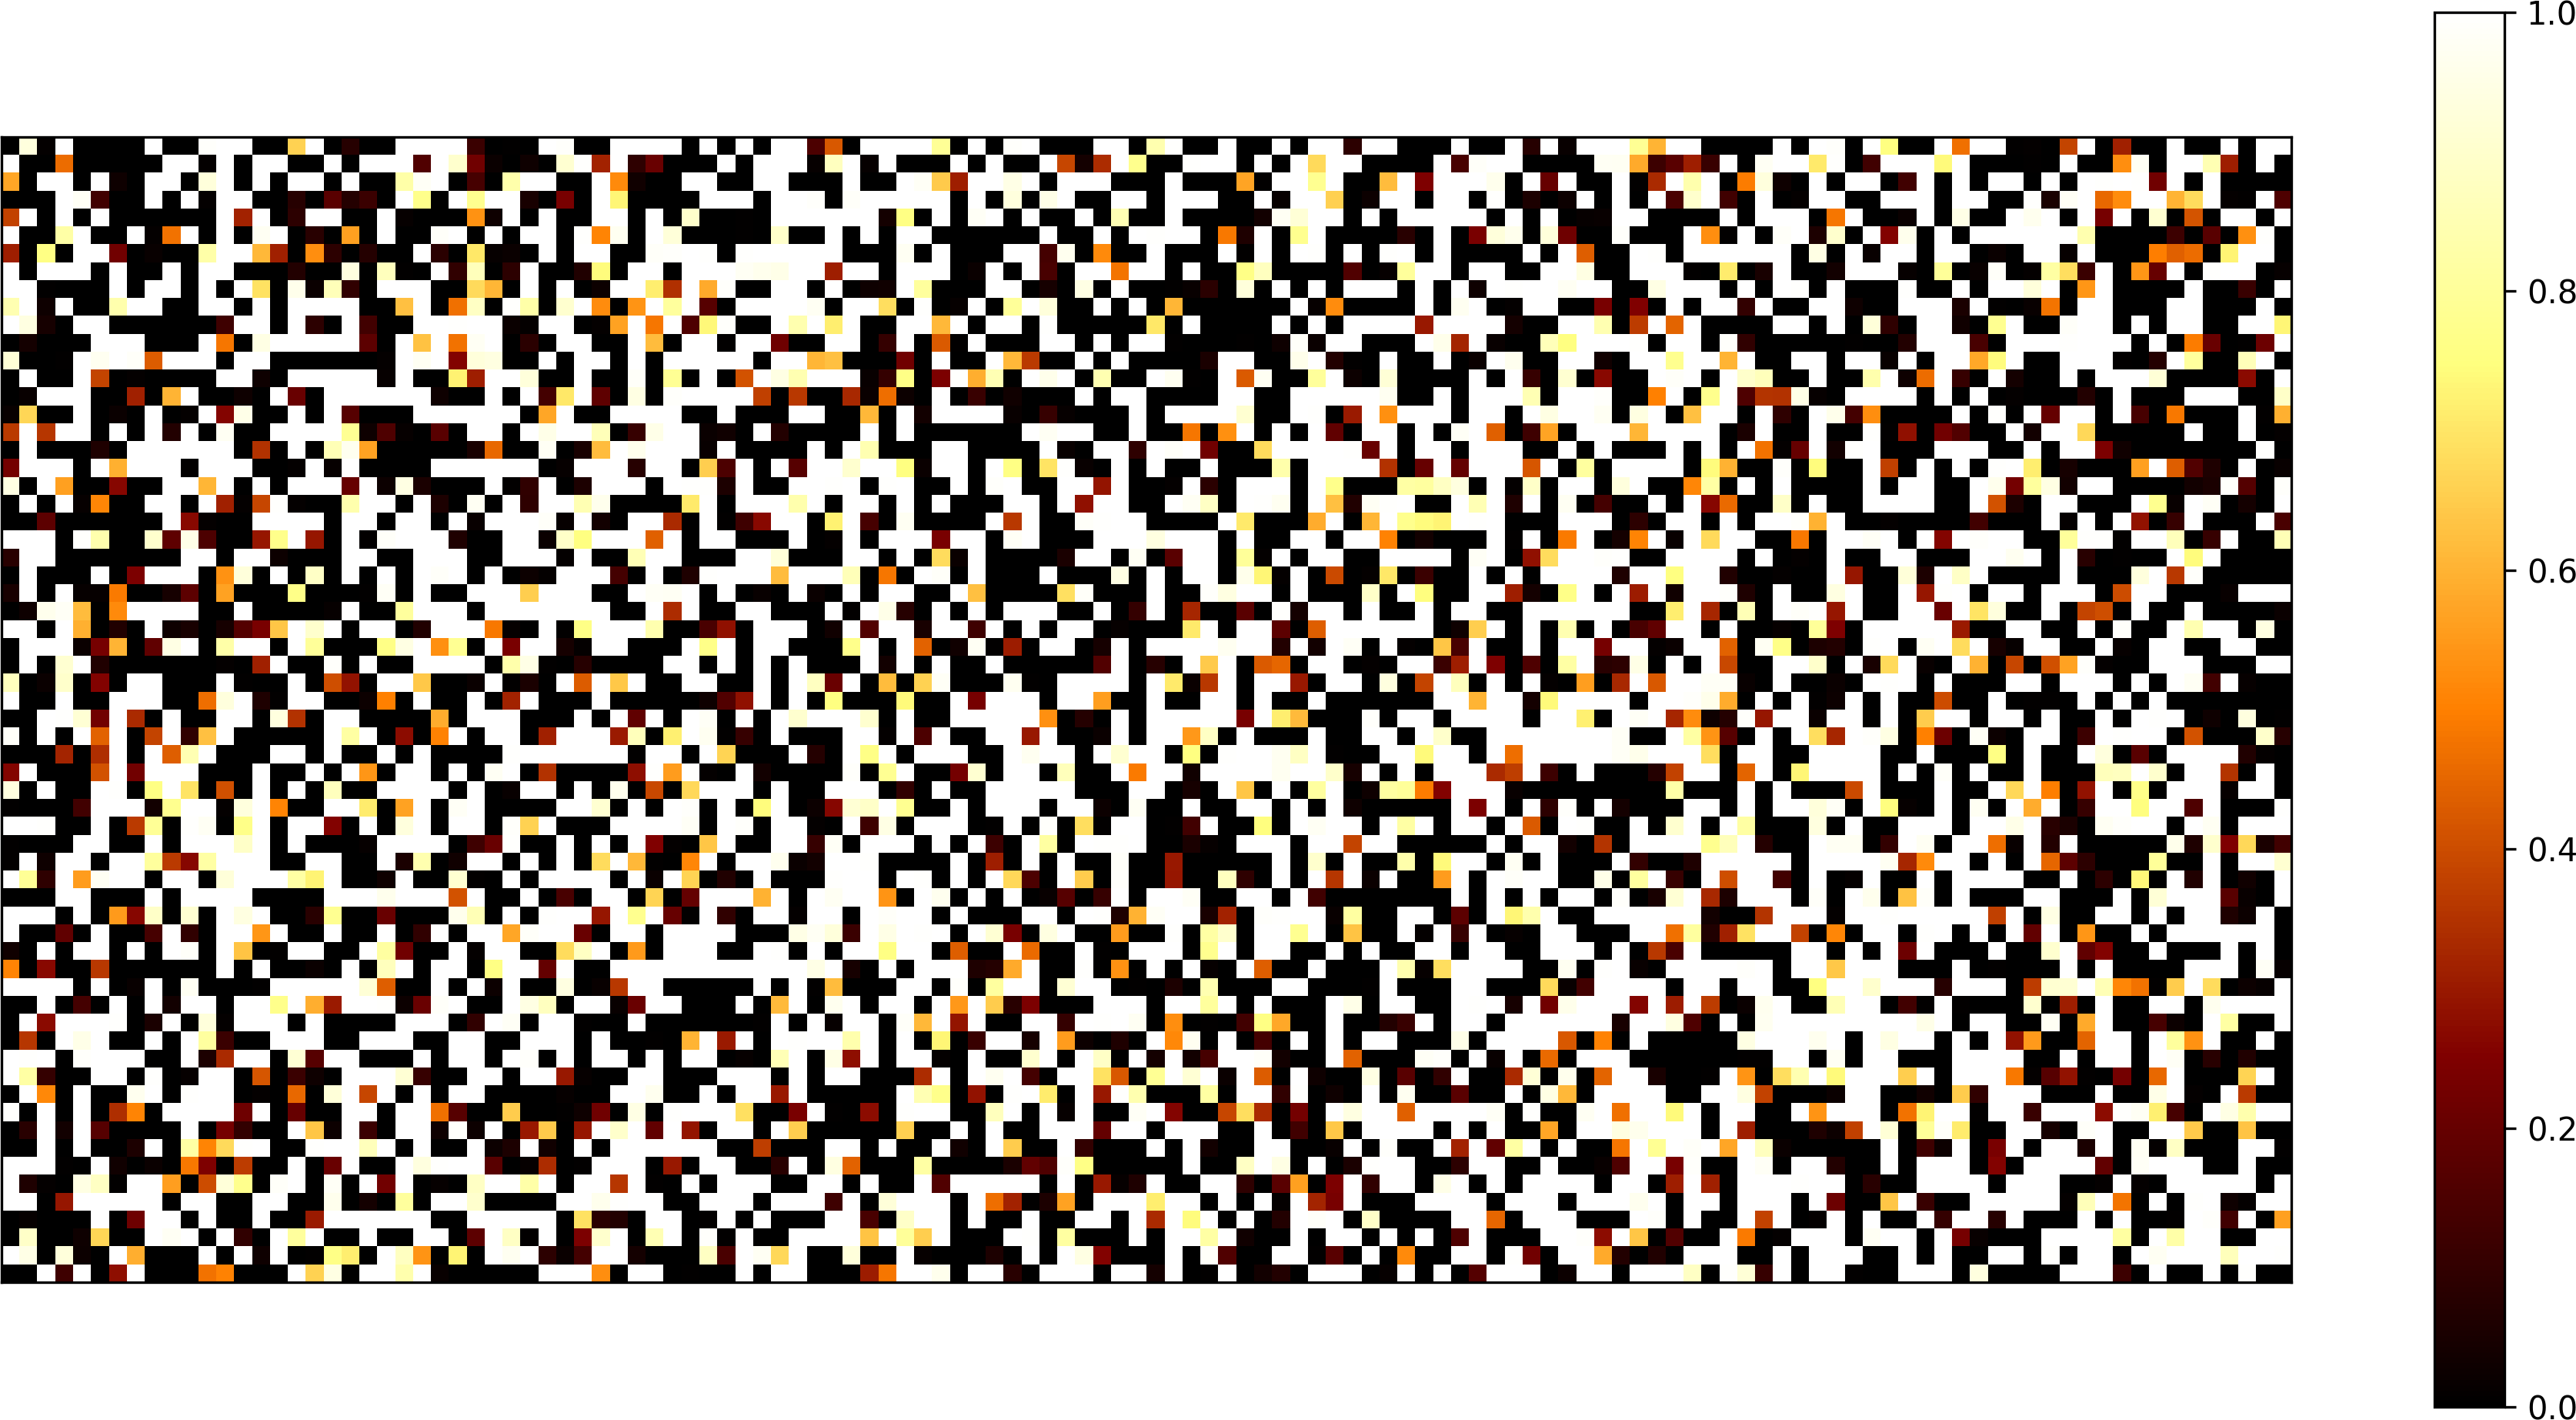
\includegraphics[width=\textwidth]{images/bit_stability.png}
    \caption[Average startup values of individual SRAM cells over 1000 measurements]{Average startup values of individual SRAM cells over 1000 measurements. White bits are stable `1', black bits are stable `0' and the rest are unstable bits with varying amounts of bias (according to the color bar on the right). Cells with an average value of 0.5 are the least stable. The data was obtained from ESP32 number 12 at 20°C.}
    \label{fig:bit_stability_mask}
\end{figure}

\subsubsection*{Indirect bit preselection}\label{sec:indirect_bit_preselection}

Indirect preselection runs a test for each bit to identify its stability. For example, a stable bit can be identified by the time it takes for it to stabilize its initial state---stable bits stabilize faster than unstable ones. The test can be performed in the following way.

First, set all the bits to the `0' state. Then, turn off the memory for a short amount of time and look at which bits flipped to the `1' state the fastest. They are the stable `1' bits. Stable `0' bits can be obtained respectively. It has been shown by~\cite{Liu2017} that up to 100\% stable response can be extracted by this method.

\section{SRAM aging}

Normal operation of \gls{sram} memory unavoidably alters its physical properties. These processes can affect the stability of \gls{sram} \gls{puf} and are called silicon aging.

The dominant effect which directly alters the stability of memory cells is called \gls{nbti}. \gls{nbti} is a data-dependent aging effect. If the cell stores a `1' bit, its startup state preference slowly starts to change towards the `0' state. This is the result of a threshold voltage increase on the transistors which are switched on in the current state, whereas the switched off transistors are unaffected. This means, that the \gls{sram} \gls{puf} has a natural tendency to become less stable over time if the startup data is left unchanged in memory.~\cite{Roelke2018}

Anti-aging techniques, which try to counteract \gls{nbti} and other effects, exist. A simple example is to store an inverse of the startup data after response extraction. However, this is a security risk as leakage of this data would directly reveal the startup memory values. Another solution could be to overwrite the memory with a random string after every power up. This results in less effective anti-aging, but avoids the security risk of a data leak.~\cite{Maes2014}

\section{Related work}

Since the main objective of this thesis is to analyze the possibility of implementing a \gls{sram} \gls{puf} on the ESP32 microcontroller, it is important to look at the already existing solutions.

The authors of~\cite{Deutschmann2018} have performed an analysis of \gls{sram} \gls{puf} implementations on existing \gls{iot} platforms. ESP32 was among the analyzed technologies. However, the information presented is extremely limited. The mechanism by which they obtained the \gls{puf} responses is not known and the operating conditions during the analysis were not specified. Furthermore, the analysis was performed using only two ESP32 microcontrollers. They also present uniformity and reliability evaluation of the \gls{puf}, though their results differ significantly from the findings in this thesis (presented in Chapter~\ref{sec:implementation}).

\cite{Javier2020} proposed a solution for secure management of \gls{iot} devices based on blockchain non-fungible tokens. In their research, the blockchain account seed was not stored digitally but was reconstructed using a \gls{sram} \gls{puf}. A proof of concept was developed and tested on three ESP32 development boards. They successfully reconstructed the seed using direct stable bit preselection and a repetition \gls{ecc}. However, the \gls{puf} was not tested in different operating conditions and no evaluation parameters were used.

To summarize, proof of concept \gls{sram} \gls{puf} implementations on the ESP32 microcontroller exist, though not enough information about how the implementations work has been provided. To the best of our knowledge, an analysis of performance of \gls{sram} \glspl{puf} on ESP32 in different operating conditions has not been published yet.


%---------------------------------------------------------------
\chapter{ESP32 platform}
%---------------------------------------------------------------


%---------------------------------------------------------------
\chapter{SRAM PUF implementation on ESP32}\label{sec:implementation}
%---------------------------------------------------------------

% uvod s tim ze pouzivam esp32, cislovani, jake desky?, komoru, jake teploty?, nominal voltage...

The goal of this chapter is to find a suitable mechanism for \gls{sram} power state control on the ESP32 microcontroller. Two different methods are presented and their result (the startup memory values used as a \gls{puf} response) are analyzed. 

First, an analysis based on temperature and \gls{sram} power off-time is performed. The temperature is controlled by a temperature chamber Binder MK-56obj. It is capable of producing temperatures from -40 °C to +180 °C\cite{Binder2021}. However, only the range of -40 °C to +70 °C is used for the analysis as higher temperatures could potentially damage the components. This analysis is performed mainly to understand the data retention time of the \gls{sram} and set an adequate minimum interval the memory needs to stay off before extracting the response.

Then, some of the \gls{puf} parameters defined in Section~\ref{sec:puf_evaluation} are used to evaluate the results. A summary of both power state control methods is provided at the end, discussing their advantages, disadvantages and viability of use.

Only the original ESP32 microcontroller model is used. Sixteen pieces will be measured and they are numbered from \gls{mcu} 1 to \gls{mcu} 16. All of the measurements were captured under normal voltage conditions. 

%--------------------------------
\section{RTC SRAM based PUF}
%--------------------------------

The first method of \gls{sram} power control is to use the \gls{rtc} part of \gls{sram} memory on ESP32. This part of memory can be switched on and off using the \gls{rtc} power domain controller.
 
\subsection{RTC SRAM power control}

The ESP32 has the ability to power-control parts of its chip. This feature can be used to save power while some of the components of the microcontroller are not being used. WiFi, digital core, internal \gls{sram} and \gls{rtc} \gls{sram} can all be power-controlled. This seems like an ideal mechanism for implementing the \gls{sram} \gls{puf} as the memory can be turned off and on during runtime with little time overhead.\cite{esp322021}

All of the individual \gls{sram} sections (SRAM 0, 1 and 2, \gls{rtc} FAST \gls{sram} and \gls{rtc} SLOW \gls{sram}, described in more detail in Section~\ref{sec:memory_layout}) can be power-controlled individually. One of the sections, therefore, needs to be selected for the \gls{puf} implementation.

At first, the logical \gls{sram} section to select would be the \gls{sram} 0, 1 or 2, as they have a large capacity (all three more than 100 KB). However, all of the data saved in the selected section would be lost during response extraction (the memory needs to be turned off). This would prohibit this chunk of memory from being used and potentially render some memory-hungry applications impossible to be implemented. Additionally, the ESP-IDF toolchain would need to be adjusted to not use this part of memory. 

\begin{figure}[ht!]
    \centering
    \captionsetup{justification=centering,margin=0.5cm}
    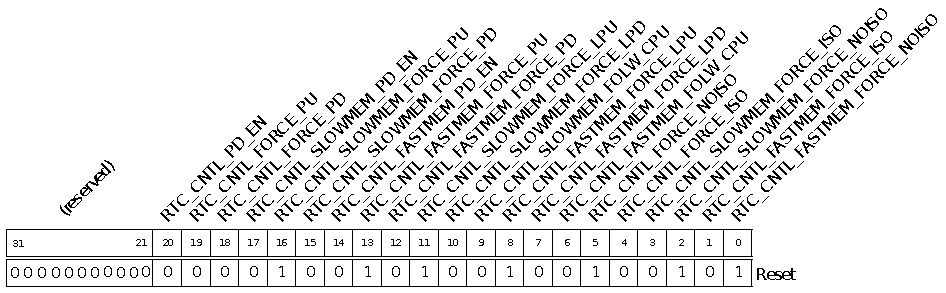
\includegraphics[width=\textwidth]{images/rtc_register.pdf}
    \caption[RTC domain power management register (address 0x3FF48080).]{RTC domain power management register (address 0x3FF48080).\cite{esp322021}}
    \label{fig:rtc_register}
\end{figure}

Because of these drawbacks, the \gls{rtc} FAST \gls{sram} section was selected. Since it is also used to store program instructions (the deep sleep wake stub) and data (dynamic heap allocations), it needs to be preserved during response extraction. This can be done by backing up the whole 8 KB section of memory to the main \gls{sram} before powering down and restoring it afterwards. This is not possible with the main \gls{sram} sections because of their size.

The power state of the FAST \gls{rtc} \gls{sram} is controlled by the \gls{rtc} domain power management register. Functions of the individual register bits are shown in Figure~\ref{fig:rtc_register}. Bits number 13 (RTC\_CNTL\_FASTMEM\_FORCE\_PU)\footnote{RTC\_CNTL\_FASTMEM\_FORCE\_PD = \gls{rtc} control fast memory force power up} and 12 (RTC\_CNTL\_FASTMEM\_FORCE\_PD)\footnote{RTC\_CNTL\_FASTMEM\_FORCE\_PD = \gls{rtc} control fast memory force power down} are important. They can be set to control the power state of the memory.\cite{esp322021}

\subsection{SRAM analysis based on temperature and power-off time}\label{sec:rtc_analysis}

Data remanence of the \gls{rtc} FAST \gls{sram}, power controlled using the above-described method, is analyzed in this section. Several experiments for each \gls{mcu} have been conducted according to this algorithm:

\begin{enumerate}
    \item Set the ambient temperature to the desired value.
    \item Initialize memory to a default value.\footnote{In the presented experiments, the default value was `0' for all bits. However, measurements with bits initialized to `1' showed nearly identical results.}
    \item Turn memory off for a set interval and then turned it on again.
    \item Observe the contents of memory.
    \item Continue from step 2. with an increased turn off interval until enough data is collected.
\end{enumerate}

Observing the contents of memory, in this case, means calculating the percentage of bits that flipped to a different state while turned off. For the default initial state of `0', this is equivalent to calculating the percentage Hamming weight of the bit string (counting the `1' bits).

The expected result is that, at the beginning for a very small turn off interval, no bits will flip. The biggest interval under which no bits flip is the \emph{data remanence time}. With increasing turn off interval, more and more bits start to flip. The percentage of flipped bits should stabilize around 50\% which is the ideal value of uniformity. At this point, all data previously saved in memory should be lost and the contents of memory after power up should depend only on the preferred initial state of the memory cells. The smallest interval under which this happens will be called the \emph{fade-out time}. The \gls{sram} \gls{puf} implementation should set the turn off interval to a greater value than the maximum \emph{fade-out time} of the \gls{sram} under varying conditions (such as temperature or voltage). This prevents data remanence from affecting the \gls{puf} response.

The results of the first experiment are displayed in Figure~\ref{fig:all_plus_20_rtc}. The graph shows the percentage of flipped bits at 20 °C with the turn off interval ranging from 0 to 1000 $\mu{}S$. The results are as expected. The \emph{data remanence time} is around 180 $\mu{}S$, the \emph{fade-out time} is around 900 $\mu{}S$ and the percentage of flipped bits stabilizes around 50\% for all \glspl{mcu}.

\begin{figure}[ht!]
    \centering
    \captionsetup{justification=centering,margin=0.5cm}
    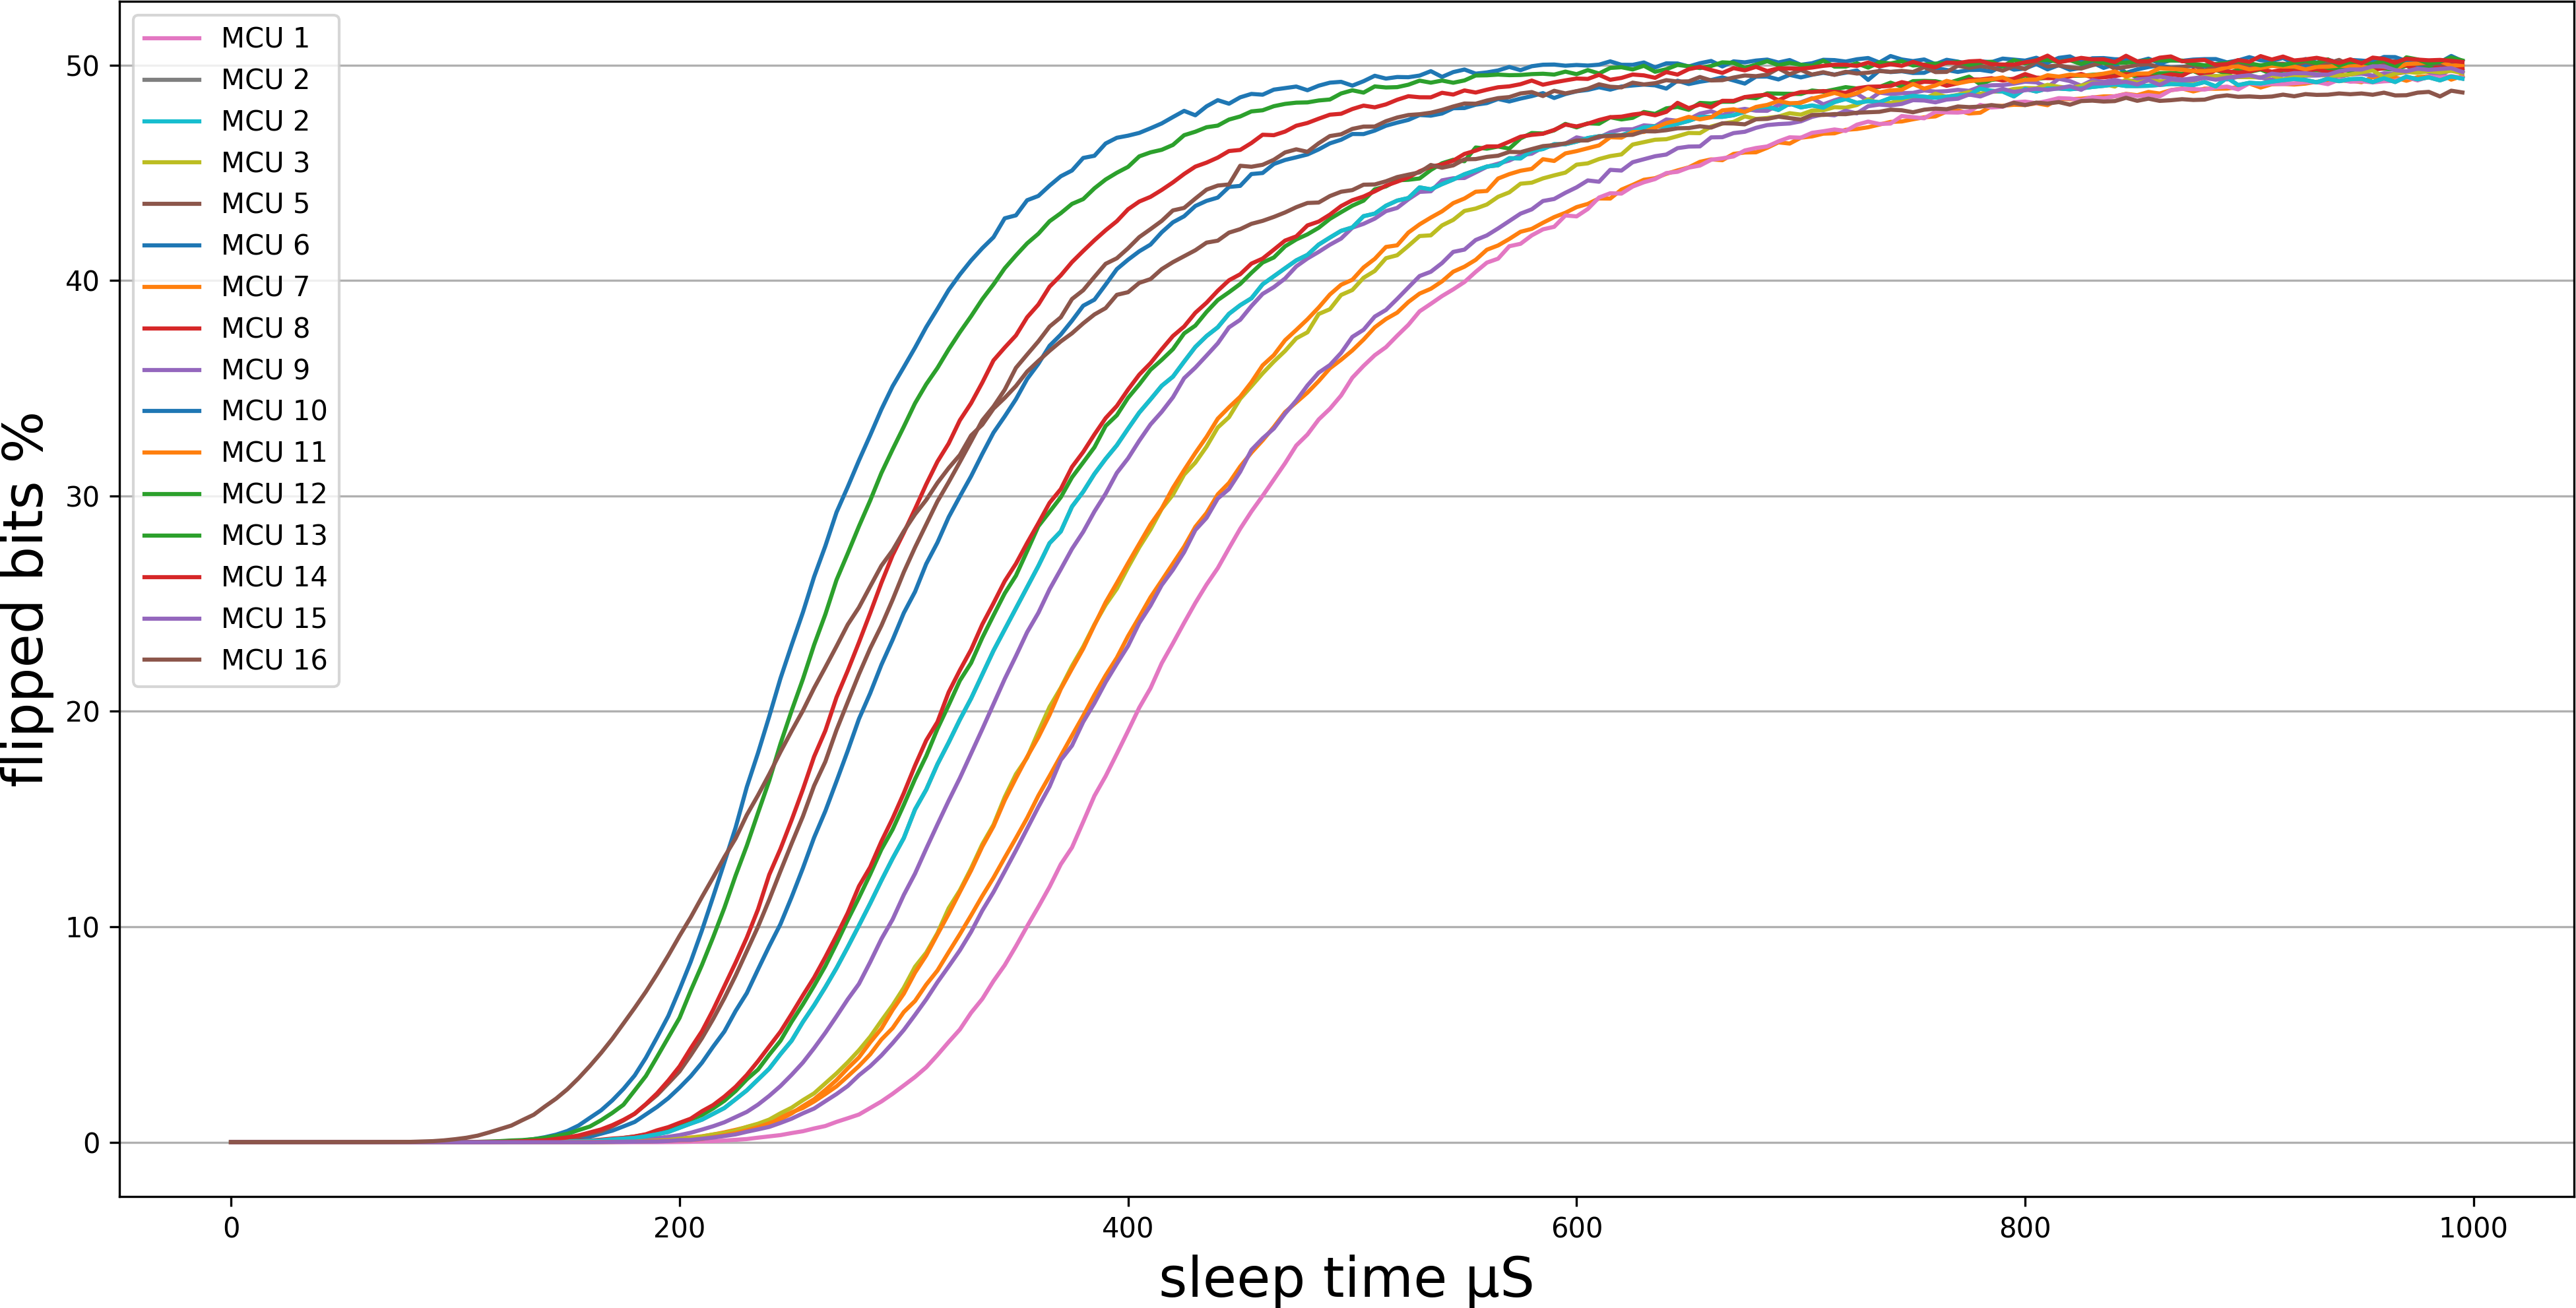
\includegraphics[width=\textwidth]{images/all_plus_20_rtc.png}
    \caption{Percentage of flipped bits of all MCUs at 20 °C (RTC SRAM method).}
    \label{fig:all_plus_20_rtc}
\end{figure}


The second experiment shows the behavior of one \gls{mcu} (number 6 was chosen but results for the others are similar) across the whole range of -40 to +70 °C. The graph can be seen in Figure~\ref{fig:6_across_temps_rtc}. As expected, the lower temperatures increase the \emph{data remanence time} and the \emph{fade-out time} significantly and higher temperatures decrease them. However, for the lower temperatures (below 0 °C), the \emph{fade-out time} cannot be seen as the memory did not have enough time to stabilize yet. 

\begin{figure}[ht!]
    \centering
    \captionsetup{justification=centering,margin=0.5cm}
    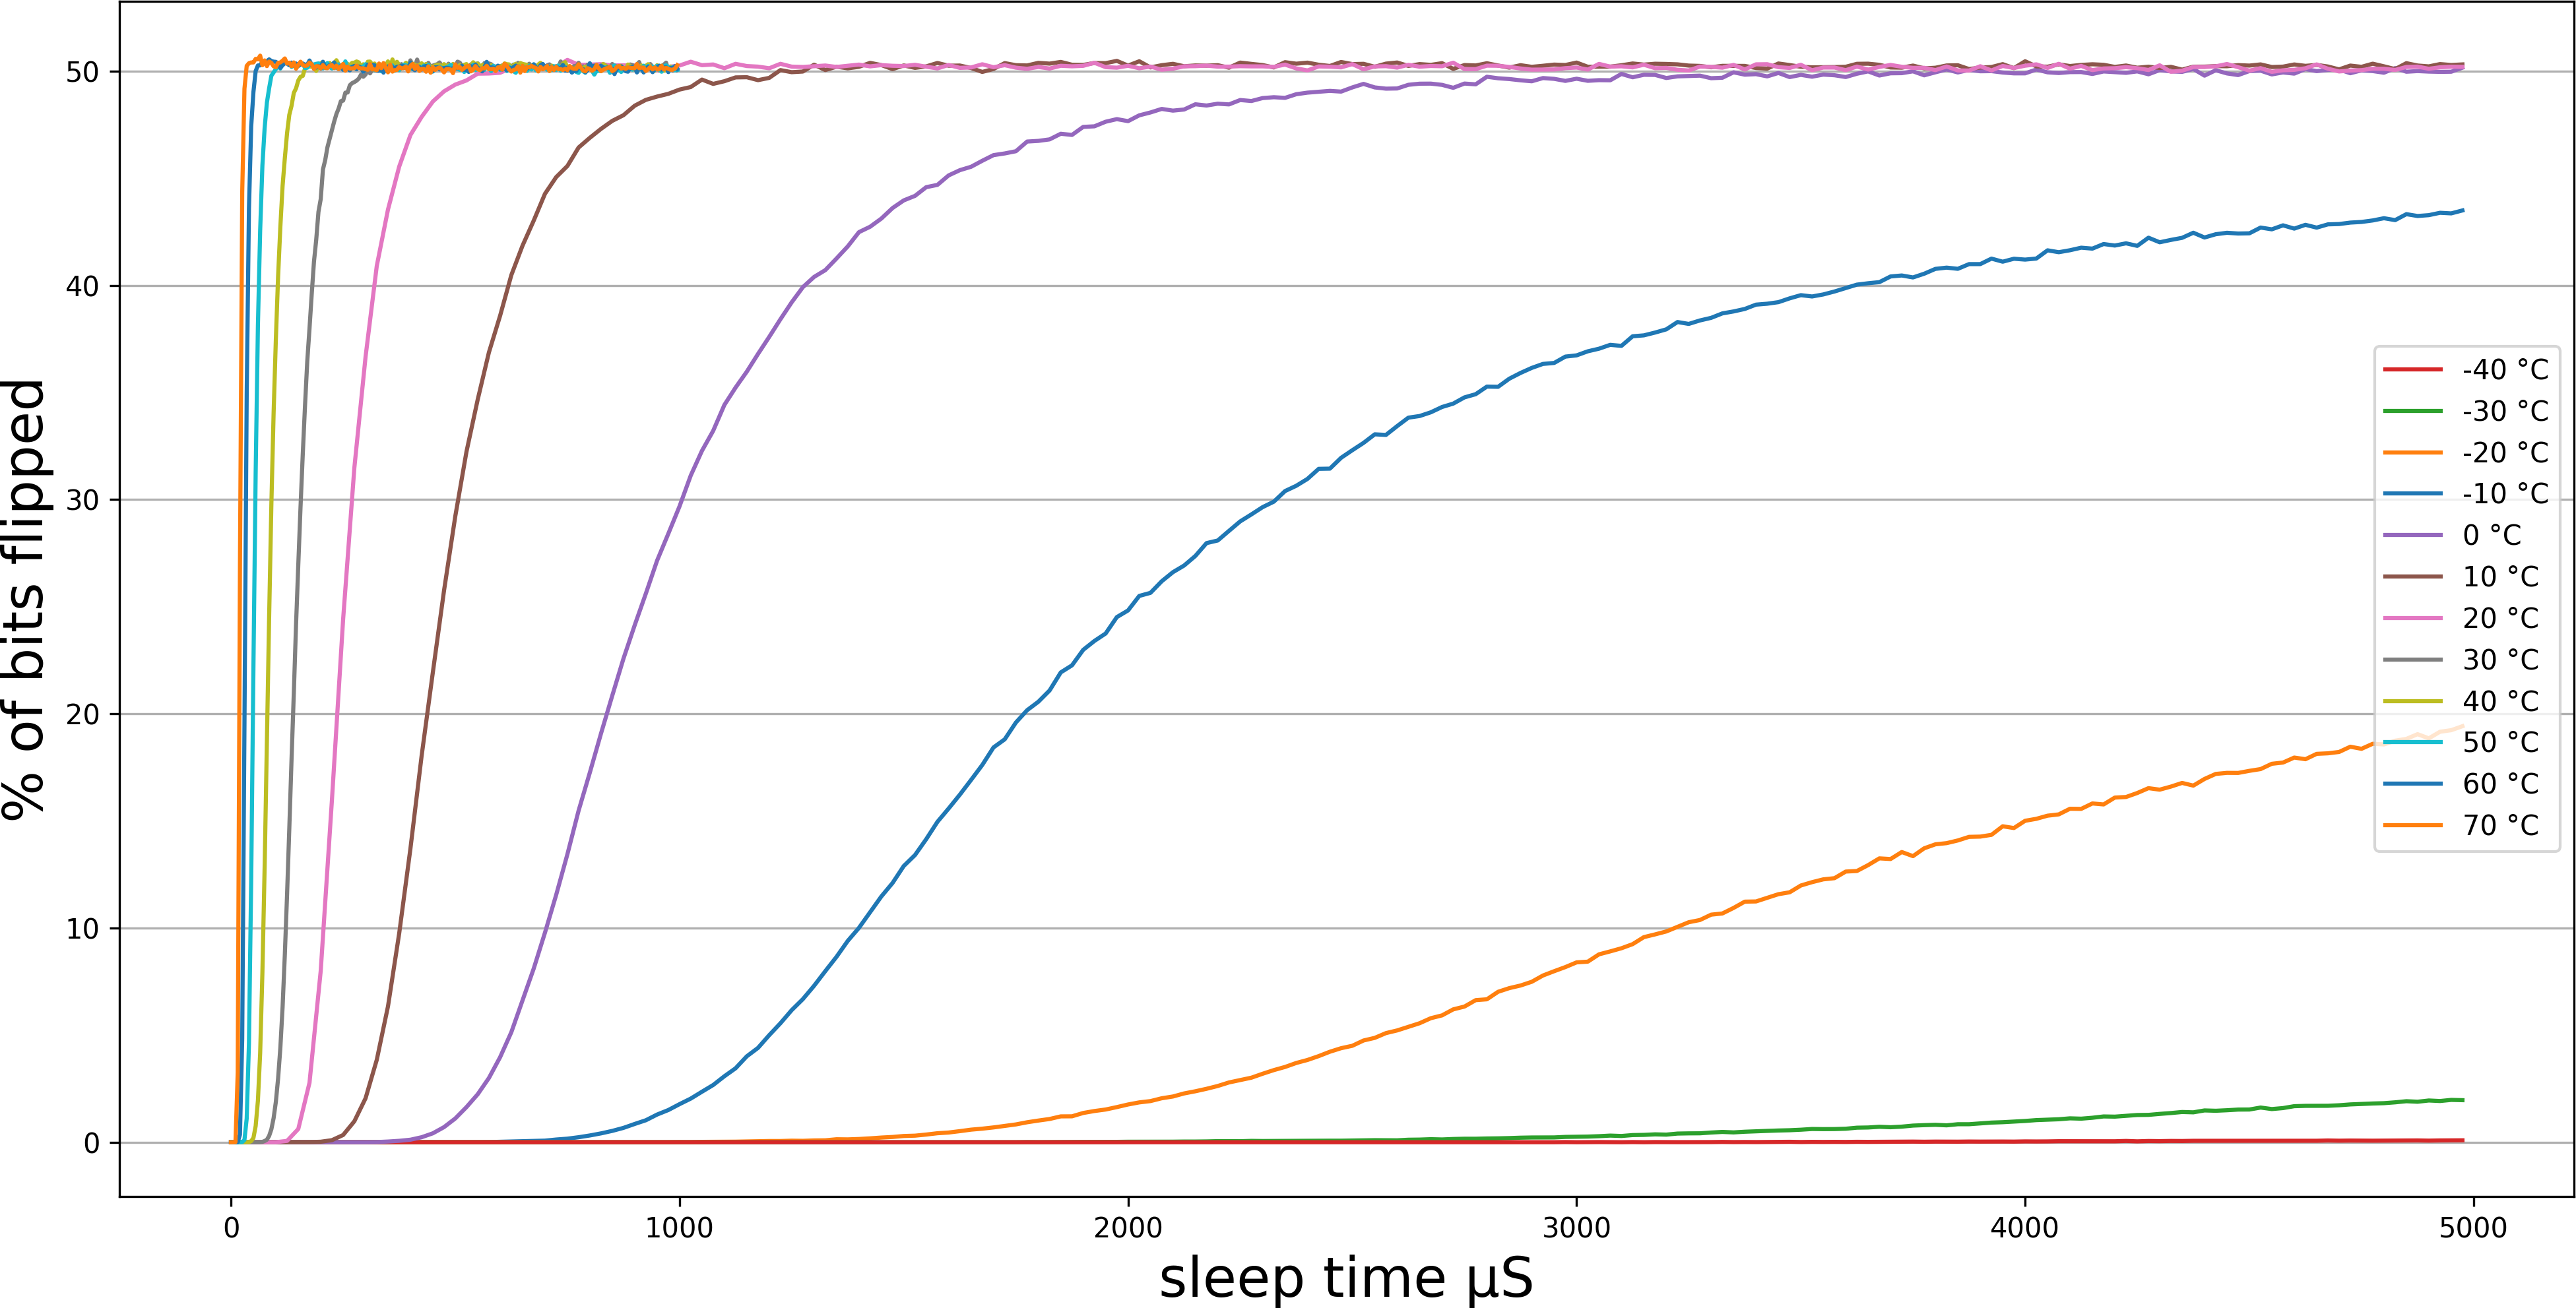
\includegraphics[width=\textwidth]{images/6_across_temps_rtc.png}
    \caption{Percentage of flipped bits of MCU 6 across a range of temperatures (RTC SRAM method).}
    \label{fig:6_across_temps_rtc}
\end{figure}

The next experiment, therefore, looks at the behavior of all \glspl{mcu} at -20 °C. The turn off interval was significantly increased to 50 000 $\mu{}S$. The results are displayed in Figure~\ref{fig:all_minus_20_rtc}. A very strange behavior can be seen. It looks as if the memory does not fade-out at all, only a limited number of bits flip and the rest of the bits retain their original state. Furthermore, for each board, a wildly different number of bits flip in this temperature. Nearly no bits flip for \gls{mcu} 4, but about 33 percent of bits flip for \gls{mcu} 6.\footnote{Note the values on the Y-axis of the graph, they do not even reach 50 \%.}

This was confirmed by extending the range of the turn off interval to 1 S and then to 100 S. The number of flipped bits does not change anymore with increased turn off time and the memory `freezes'. At -40 °C only about 1 \% of bits flip no matter the turn off interval for each \gls{mcu}. The initial value of the memory cell does not matter either, `0' and `1' states both freeze in the same way. 

\begin{figure}[ht!]
    \centering
    \captionsetup{justification=centering,margin=0.5cm}
    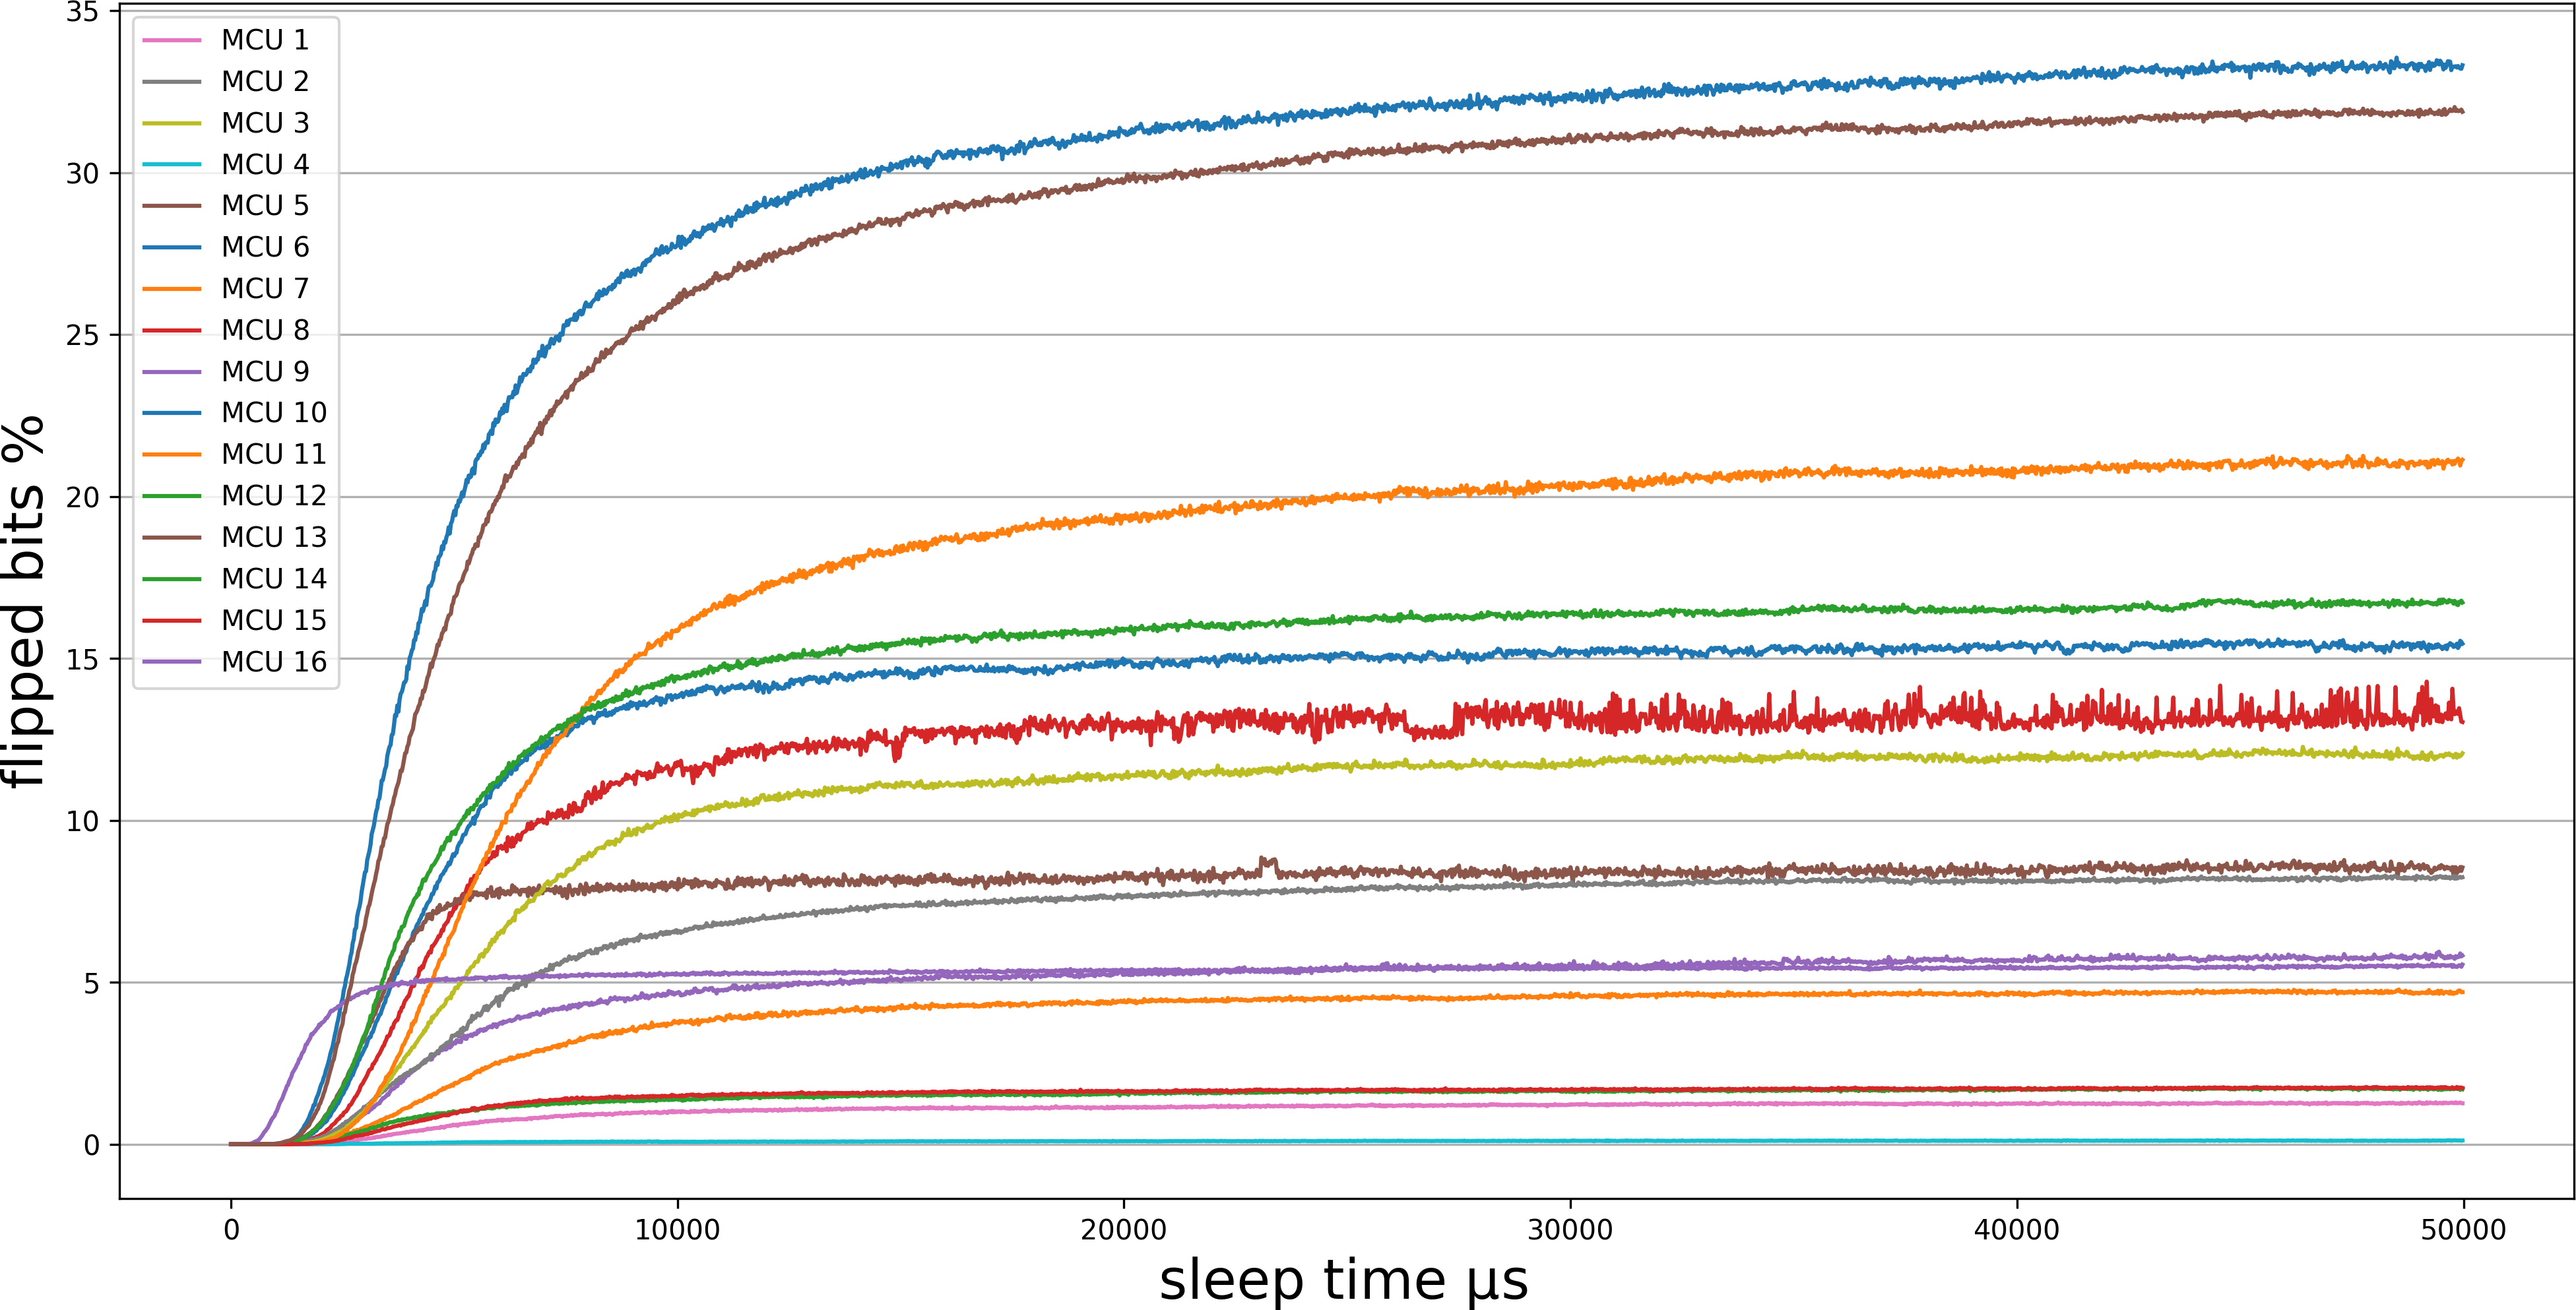
\includegraphics[width=\textwidth]{images/all_minus_20_rtc.png}
    \caption{Percentage of flipped bits of all MCUs at -20 °C (RTC SRAM method).}
    \label{fig:all_minus_20_rtc}
\end{figure}

A possible explanation of this behavior can be the following. All transistors leak current even if they are switched off. This is called a leakage current. A transistor that works as a switch for turning the \gls{rtc} FAST \gls{sram} on and off has a leakage current that is high enough that the memory is able to retain its state in low temperatures. \gls{sram} memory draws very little power while only retaining data---no read/write operations are taking place and thus the logical states of the circuit do not change. This is called static \gls{cmos} power dissipation. It has been shown by \cite{Kocanda2015} that the static power dissipation is highly influenced by temperature. A change of temperature from 100 to 20 °C decreases the power draw by a factor of 3 to 83, depending on the exact \gls{cmos} technology used.

As is evident from the Figure~\ref{fig:all_minus_20_rtc}, different \glspl{mcu} freeze at different rates---the percentage of bit flips varies wildly across \glspl{mcu}. This supports this hypothesis as the leakage current of the transistor is probably also influenced by the random variations during the manufacturing process.

This can explain the `freezing' effect of memory in low temperatures. However, this explanation could not be confirmed.

\subsection{PUF evaluation parameters}\label{sec:rtc_evaluation}

Since the evaluation parameters require \gls{puf} responses for their calculation, they need to be obtained. The response was chosen to be a 4 KB bit string of the (first half of) \gls{rtc} FAST \gls{sram}. Only one response is extracted, no memory address based challenge system was considered because of the limited size of the used memory region (8 KB). The turn off interval was set to 10 000 $\mu{}S$. This is a lot higher value than the \emph{fade-out time} of the memory for warmer temperatures (above 0 °C). There is no point in considering lower temperatures since the memory freezes while using this power control technique. The reference response was calculated using a bitwise average of 1000 measured responses.

\subsubsection*{Uniformity}

Uniformity of all \glspl{mcu} in different temperatures can be seen in Table~\ref{table:uniformity_rtc_sram}. The values look very good at temperatures above 10 °C, hovering around the desired value of 50 \%. However, in lower temperatures, the effect of memory freezing can be seen clearly. The values plummet and hit nearly 0 \% at -40 °C. This is due to the choice of default initial value of `0' bits. Uniformity rises towards 100 \% if the default value is a `1' bit.

\begin{table}[ht!]
    \centering
    \begin{tabular}{c||rrrrrrrrrr}
\toprule
\textbf{MCU} & \textbf{-40°C} & \textbf{-30°C} & \textbf{-20°C} & \textbf{-10°C} & \textbf{0°C} & \textbf{10°C} & \textbf{20°C} & \textbf{30°C} & \textbf{50°C} & \textbf{70°C} \\
\midrule
1    &   0.00 &   0.06 &   1.26 &  10.27 & 38.00 & 48.94 & 49.93 & 49.89 & 49.92 & 49.91 \\
2    &   0.05 &   0.55 &   8.32 &  25.05 & 44.08 & 49.29 & 49.52 & 49.65 & 49.81 & 49.88 \\
3    &   0.23 &   1.88 &  12.06 &  34.63 & 46.89 & 49.76 & 49.92 & 49.91 & 49.98 & 49.99 \\
4    &   0.00 &   0.00 &   0.10 &   2.74 & 14.74 & 41.72 & 49.95 & 50.18 & 50.36 & 50.38 \\
5    &   0.16 &   1.85 &   8.09 &  27.40 & 44.46 & 49.96 & 50.02 & 50.06 & 50.11 & 50.12 \\
6    &   1.11 &  10.82 &  33.17 &  47.60 & 50.11 & 50.18 & 50.09 & 50.08 & 50.06 & 50.04 \\
7    &   0.45 &   7.71 &  21.45 &  39.26 & 49.45 & 50.11 & 50.17 & 50.20 & 50.29 & 50.29 \\
8    &   0.18 &   2.41 &  14.03 &  25.69 & 45.20 & 49.96 & 49.84 & 49.92 & 49.98 & 50.00 \\
9    &   0.07 &   0.57 &   5.69 &  20.71 & 39.98 & 49.14 & 49.76 & 49.79 & 49.78 & 49.82 \\
10   &   0.17 &   2.91 &  15.35 &  37.38 & 48.65 & 49.83 & 49.96 & 49.99 & 50.03 & 50.04 \\
11   &   0.05 &   0.40 &   4.75 &  23.70 & 43.60 & 49.88 & 50.24 & 50.18 & 50.26 & 50.31 \\
12   &   0.00 &   0.07 &   1.63 &  16.19 & 38.21 & 48.25 & 49.96 & 49.96 & 49.89 & 49.86 \\
13   &   0.80 &  12.58 &  31.70 &  44.66 & 49.76 & 49.98 & 50.08 & 50.10 & 50.07 & 50.01 \\
14   &   0.18 &   2.44 &  16.75 &  39.50 & 49.43 & 50.09 & 50.16 & 50.19 & 50.14 & 50.17 \\
15   &   0.01 &   0.11 &   1.74 &  17.96 & 36.05 & 48.30 & 50.13 & 50.18 & 50.17 & 50.13 \\
16   &   0.77 &   2.02 &   5.48 &  13.92 & 30.52 & 44.13 & 49.55 & 49.74 & 49.81 & 49.90 \\
\textbf{mean} &   0.27 &   2.90 &  11.35 &  26.67 & 41.82 & 48.72 & 49.96 & 50.00 & 50.04 & 50.05 \\
\bottomrule
\end{tabular}
    \captionsetup{justification=centering,margin=0.5cm}
    \caption{Uniformity (\%) across all MCUs and temperatures (RTC SRAM method).}
    \label{table:uniformity_rtc_sram}
\end{table}

\subsubsection*{Reliability}

Reliability values of all \glspl{mcu} in different temperatures are displayed in Table~\ref{table:reliability_rtc_sram}. The reference response used for the calculations was obtained at 20°C.

Once again, the values look good in temperatures above 10 °C, being fairly close to the ideal 100 \%. The highest reliability can be observed at 20 °C. This is the result of the reference response being calculated at this temperature. The effect of freezing is once again evident in low temperatures. Reliability goes down toward 50 \%, which is the worst possible value.\footnote{The value of 0 \% would mean that the response bits are just inverted compared to the reference.} 

\begin{table}[ht!]
    \centering
    \begin{tabular}{c||rrrrrrrrrr}
    \toprule
    \textbf{MCU} & \textbf{-40°C} & \textbf{-30°C} & \textbf{-20°C} & \textbf{-10°C} & \textbf{0°C} & \textbf{10°C} & \textbf{20°C} & \textbf{30°C} & \textbf{50°C} & \textbf{70°C} \\
    \midrule
    1    &  50.16 &  52.80 &  63.34 &  80.56 & 87.36 & 93.70 & 96.55 & 95.41 & 93.96 & 93.25 \\
    2    &  49.71 &  50.06 &  54.19 &  71.71 & 88.36 & 94.19 & 97.35 & 95.71 & 93.72 & 93.06 \\
    3    &  50.04 &  50.10 &  51.61 &  65.27 & 84.11 & 89.41 & 96.99 & 93.54 & 90.39 & 89.82 \\
    4    &  50.46 &  52.60 &  62.97 &  71.01 & 81.68 & 91.70 & 96.65 & 95.61 & 94.22 & 93.65 \\
    5    &  50.33 &  50.82 &  55.72 &  68.29 & 80.18 & 90.17 & 96.75 & 94.94 & 93.05 & 92.53 \\
    6    &  50.20 &  51.86 &  57.55 &  71.77 & 81.84 & 93.09 & 96.63 & 95.67 & 94.48 & 93.81 \\
    7    &  50.08 &  50.13 &  51.27 &  59.75 & 82.78 & 90.01 & 96.86 & 94.07 & 89.99 & 88.93 \\
    8    &  50.56 &  51.04 &  58.27 &  72.19 & 83.89 & 92.07 & 96.70 & 94.55 & 91.32 & 90.30 \\
    9    &  50.29 &  51.91 &  60.69 &  79.92 & 87.22 & 93.40 & 96.75 & 95.59 & 93.94 & 93.16 \\
    10   &  50.09 &  50.09 &  50.19 &  52.76 & 64.25 & 88.26 & 97.45 & 93.60 & 88.17 & 86.39 \\
    11   &  50.91 &  59.56 &  77.59 &  86.35 & 91.16 & 94.87 & 96.38 & 95.92 & 95.14 & 94.30 \\
    12   &  50.31 &  57.04 &  68.94 &  78.72 & 86.82 & 93.98 & 96.53 & 95.81 & 94.73 & 94.08 \\
    13   &  50.69 &  61.81 &  77.67 &  81.53 & 87.42 & 95.28 & 96.65 & 96.06 & 95.22 & 94.47 \\
    14   &  50.00 &  52.19 &  65.25 &  82.92 & 89.61 & 94.80 & 96.61 & 95.70 & 94.50 & 93.70 \\
    15   &  49.89 &  49.99 &  51.60 &  66.71 & 82.06 & 89.75 & 96.94 & 93.16 & 89.77 & 89.06 \\
    16   &  51.17 &  52.33 &  55.64 &  63.53 & 78.56 & 90.84 & 98.31 & 92.24 & 80.72 & 76.13 \\
    \textbf{mean} &  50.31 &  52.77 &  60.15 &  72.06 & 83.58 & 92.22 & 96.88 & 94.85 & 92.08 & 91.04 \\
    \bottomrule
    \end{tabular}
    \captionsetup{justification=centering,margin=0.5cm}
    \caption{Reliability (\%) across all MCUs and temperatures (RTC SRAM method).}
    \label{table:reliability_rtc_sram}
\end{table}

\subsubsection*{Uniqueness}

Uniqueness of the responses from different \glspl{mcu} across the whole range of temperatures is shown in Table~\ref{table:uniqueness_rtc_sram}. Again, the values look good in temperatures above 0 °C, attacking the ideal of 50 \%. However, in lower temperatures uniqueness plummets rapidly as the responses start to freeze. Since the initial value of memory is the same across the \glspl{mcu}, the data remanence kicks in and the responses start to become more and more alike.

\begin{table}[ht!]
    \centering
    \begin{tabular}{cc}
    \textbf{Temperature °C} & \textbf{Uniqueness \%} \\
    \toprule
    -40  &  0.53 \\
    -30  &  5.63 \\
    -20  & 20.18 \\
    -10  & 39.19 \\
    0    & 48.64 \\
    10   & 49.81 \\
    20   & 49.73 \\
    30   & 49.66 \\
    40   & 49.60 \\
    50   & 49.55 \\
    60   & 49.54 \\
    70   & 49.54 \\
    \textbf{mean} & 38.47 \\
    \bottomrule
    \end{tabular}
    \captionsetup{justification=centering,margin=0.5cm}
    \caption{Uniqueness (\%) across all MCUs and temperatures (RTC SRAM method).}
    \label{table:uniqueness_rtc_sram}
\end{table}

\subsection{Summary}
% ze tohle jde jen na puvodnim ESP32 a single coru, protoze ostatni maji jiny rezim
As is evident from the experiments, this power control method can only be used at temperatures above 10 °C. The exact temperature where the memory starts to freeze also differs for each \gls{mcu}.

Moreover, only the original ESP32 and the ESP32-S2 (the single-core version) microcontrollers have the functionality to power-control the memory sections. In the newer models, this functionality was replaced by the `retention' mode of memory. This mode enables the memory to retain its data while no read/write operations need to take place, saving power in the process.\cite{esp322021} Thus, this method cannot be applied to the newer models.

On the other side, the ability to power-control the memory during runtime is very powerful. The response can be extracted on demand quickly because the whole device does not need to be powered down and then up which is an extremely time-consuming process.

%--------------------------------
\section{Deep sleep based PUF}
%--------------------------------

The second method of \gls{sram} power control is to use the internal \gls{sram} memory on ESP32. This part of memory can be switched on and off using the deep sleep mode.

\subsection{Deep sleep SRAM power control}

During the deep sleep power-saving mode, most of the chip is powered down. The \glspl{cpu}, most of \gls{sram} and all digital peripherals are turned off. Only the \gls{rtc} controller, the \gls{ulp} coprocessor and the FAST and SLOW \gls{rtc} \gls{sram} remain powered on. 

Several sources can be used to wake the device up from deep sleep. The \gls{rtc} timer, external \gls{gpio}, touch sensor and the \gls{ulp} coprocessor can all be used for this purpose. Since most of the device was turned off, the whole booting process (described in Section~\ref{sec:device_startup}) must take place during wakeup.

The \gls{rtc} timer is the wake-up mechanism that was chosen for the \gls{sram} power control, as it enables setting a precise power off interval. However, the \gls{rtc} timer uses an internal 150kHz RC oscillator as its clock source. The exact oscillator frequency is affected by temperature. This results in a time drift for different operating temperatures. Fortunately, this should not affect the \gls{puf} implementation. The same time drift will occur both in the real response extraction and during experiments. Only the power off timing information has reduced accuracy. This was not an issue while using the \gls{rtc} \gls{sram} based power control method, since the \gls{cpu} (which performed the timing) is clocked using  a 480 Mhz \gls{pll} clock.\cite{esp322021}\cite{espidf2022}

Care needs to be taken while extracting the startup memory values. As the boot process of the device is fairly complex, it is difficult to know exactly what regions of memory stay uninitialized and what regions are used by the bootloaders or the FreeRTOS before our code is executed. Even if such an uninitialized region of memory was found, it is not guaranteed that it will stay this way after a software update. The linker can assign new variables to this memory region or the old variables might be reordered. The memory would then be set to program data before we could extract the startup values.

To prevent this from happening, a process for extracting the startup values early in device boot was designed using the \emph{deep sleep wake stub}:

\begin{enumerate}
    \item After wakeup, the first stage bootloader calls the custom \emph{deep sleep wake stub} function
    \item The \emph{deep sleep wake stub} runs before the majority of other boot code. Therefore, it sees nearly the whole \gls{sram} memory uninitialized. A 4 KB of data from address 0x3FFB0000 is copied to a statically allocated buffer.
    \item The rest of the boot process continues.
    \item After boot, the startup data is found untouched in the buffer.
\end{enumerate}

The 0x3FFB0000 address (which is an address into the internal \gls{sram} 2) was chosen arbitrarily. Any address of the internal \gls{sram} 0, 1 or 2 can be chosen except for their first few KB---they are used by the first-stage bootloader before the \emph{deep sleep wake stub} runs.

The statically allocated buffer is not overwritten during the boot process because it is annotated by a \emph{NOINIT\_ATTR} attribute in the source code and is put into the \emph{no-init} section by the linker. This section is not initialized and was created to keep data during software resets.\cite{espidf2022}

Copying the data to this buffer by the \emph{deep sleep wake stub} is necessary as the \emph{no-init} section can be moved by the linker to a different memory address. This could be prevented by altering the linker script in the ESP-IDF source. Though this would make the deployment of the resulting \gls{puf} implementation significantly more difficult.


\subsection{SRAM analysis based on temperature and power-off time}\label{sec:deep_sleep_analysis}

All of the experiments shown in this section were conducted using the same method that was explained at the beginning of Section~\ref{sec:rtc_analysis}. The above-described deep sleep power-control mechanism was used and the number of bit flips was calculated from 4 KB memory samples.

The first experiment shows the percentage of flipped bits across all \glspl{mcu} at -40 °C. The lowest temperature is shown as it is the most indicative of what value to choose for the turn off interval. The resulting graph can be seen in Figure~\ref{fig:all_minus_40_deep_sleep}. The \emph{data remanence time} for the \glspl{mcu} is approximately 1 200 $\mu{}S$ (this is more evident if the graph is zoomed in) and the \emph{fade-out time} is around 50 000 $\mu{}S$.

The effect of memory freezing in low temperatures is not present while using the deep sleep power-control method, as all the \glspl{mcu} stabilize around 50 \% of flipped bits.

\begin{figure}[ht!]
    \centering
    \captionsetup{justification=centering,margin=0.5cm}
    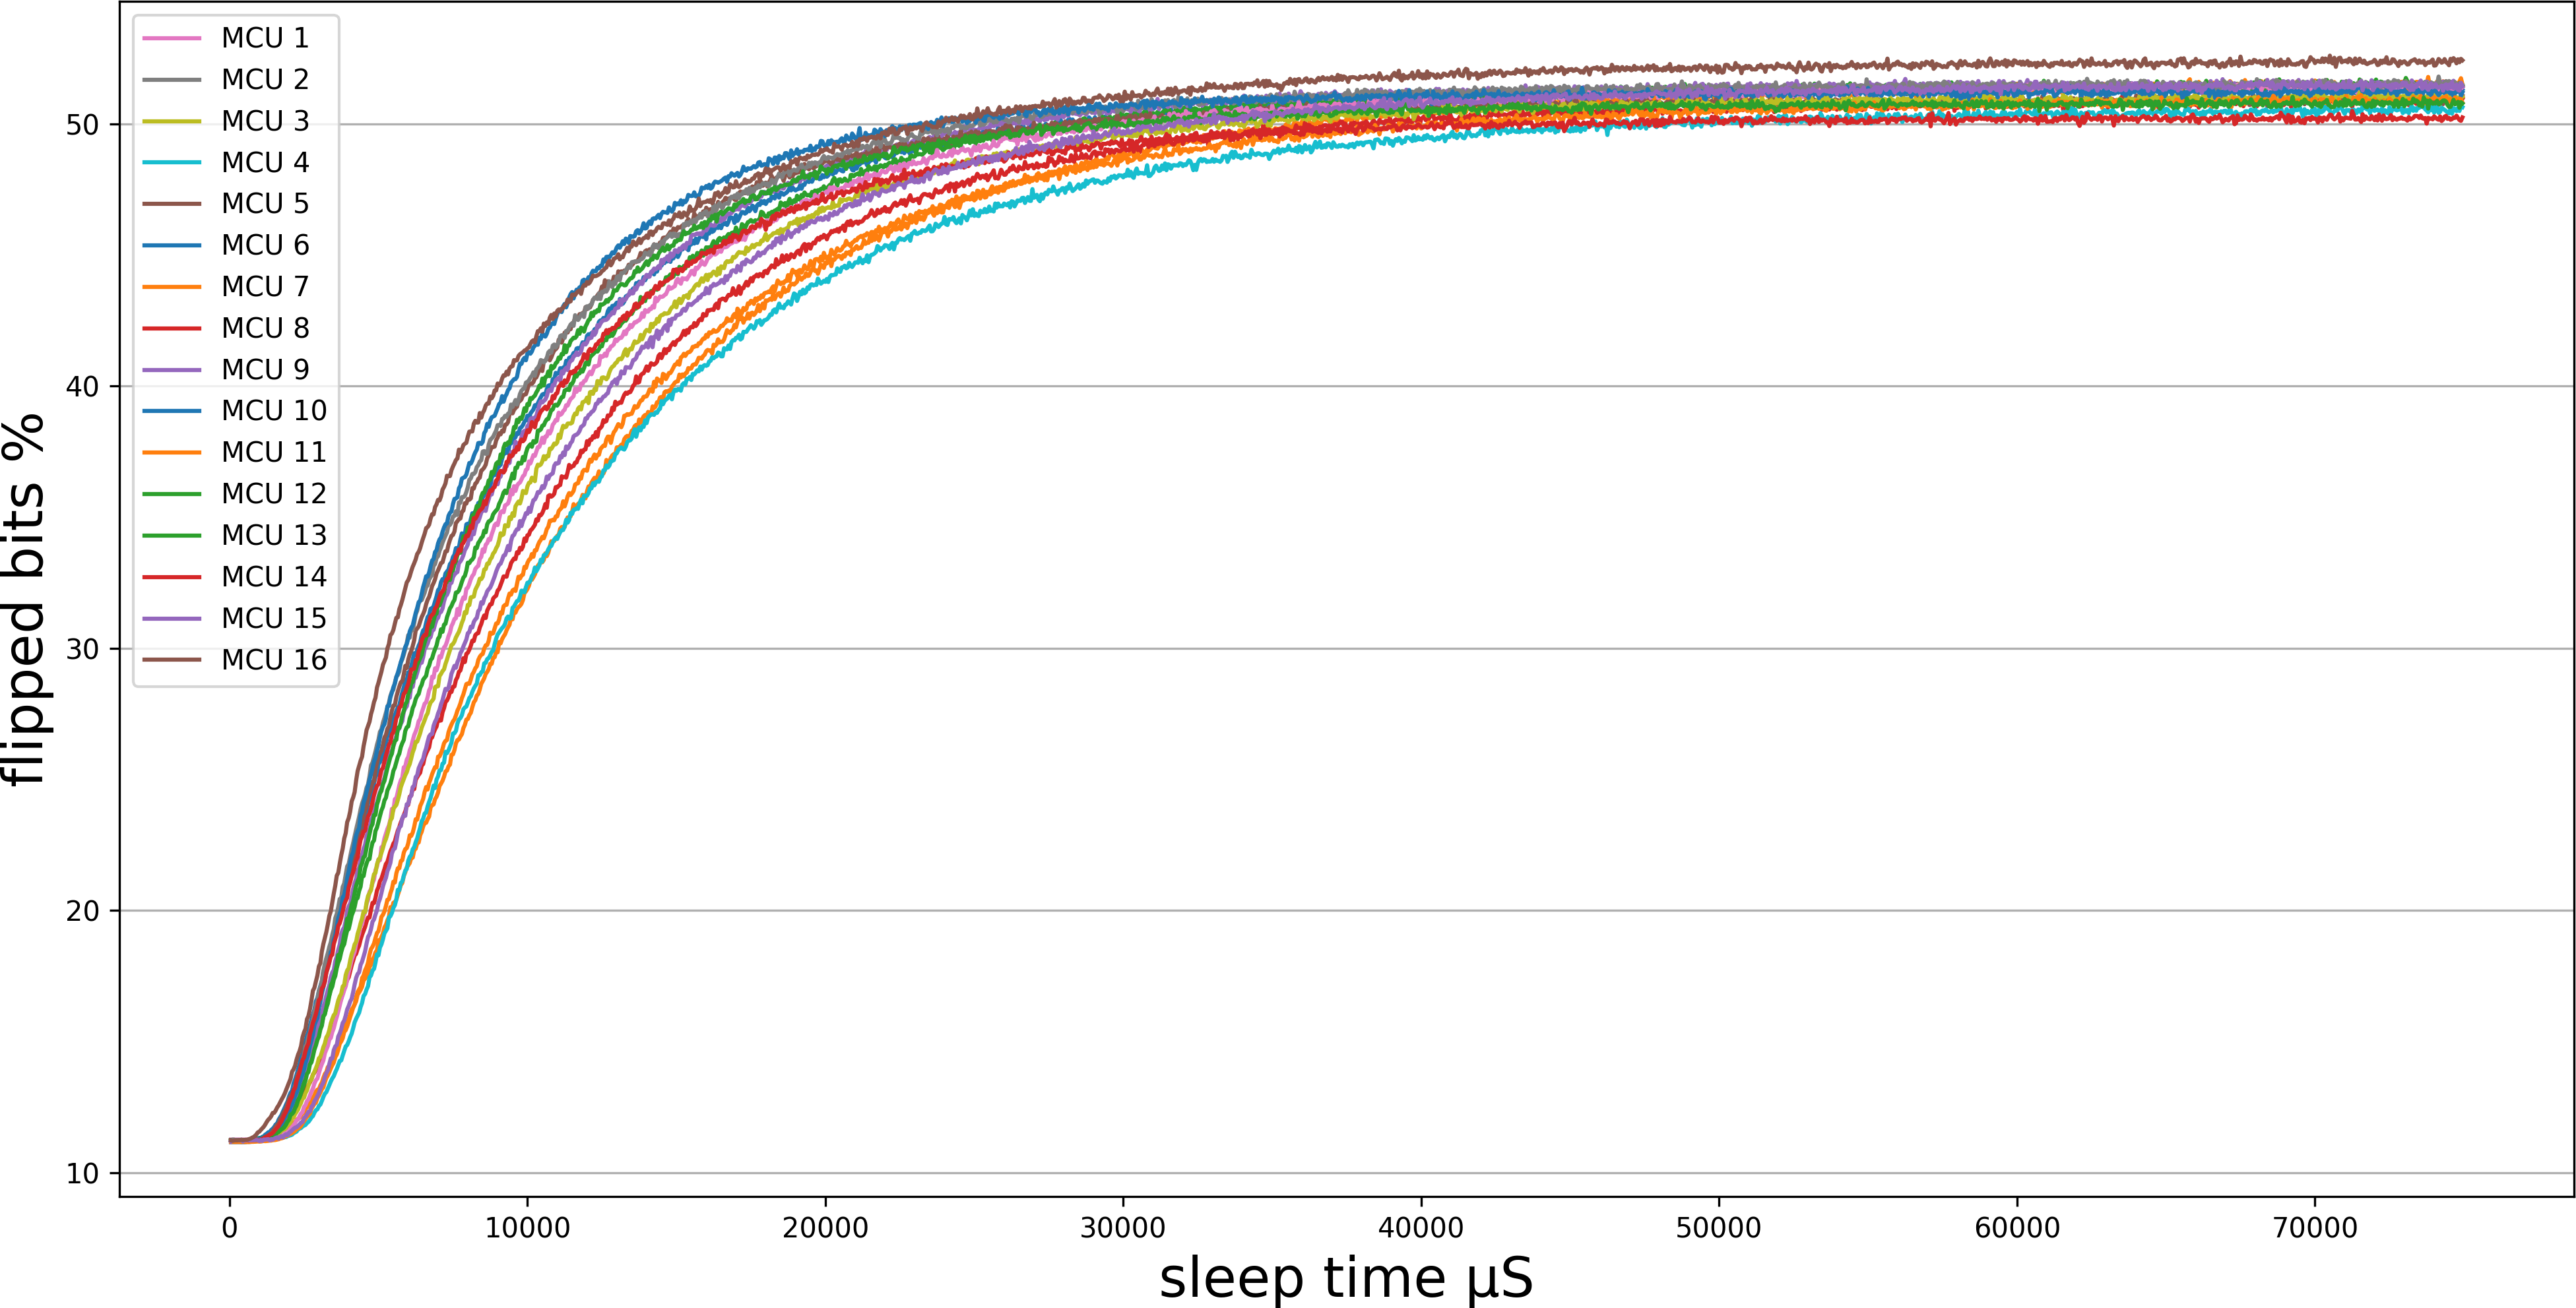
\includegraphics[width=\textwidth]{images/all_minus_40_deep_sleep.png}
    \caption{Percentage of flipped bits of all MCUs at -40 °C (deep sleep method).}
    \label{fig:all_minus_40_deep_sleep}
\end{figure}

The second experiment looks at the behavior of one \gls{mcu} (again, the number 6 was chosen but results for the others are similar) across the whole range of -40 to +70 °C. The results are shown in Figure~\ref{fig:6_across_temps_deep_sleep}. This time, since no memory freezing effect is present, the memory stabilizes around the value of 50 \% of flipped bits for all temperatures. It is also evident that the \emph{fade-out time} and the \emph{data remanence time} increase significantly with decreasing temperatures.

Note the data points for temperatures above 0 °C. Unexpectedly, they show a significant number of bit flips for very small turn off intervals (even for 0 $\mu{}S$). This behavior is caused by the \gls{rtc} controller that wakes up the chip from deep sleep. Even if the sleep time is set to 0 $\mu{}S$, the whole chip is put into deep sleep for at least 1 000 $\mu{}S$. This is probably caused by the design of the \gls{rtc} controller or the internal ESP-IDF software components. However, the deep sleep mode behaves as expected if the turn off interval is greater than 1 000 $\mu{}S$.

\begin{figure}[ht!]
    \centering
    \captionsetup{justification=centering,margin=0.5cm}
    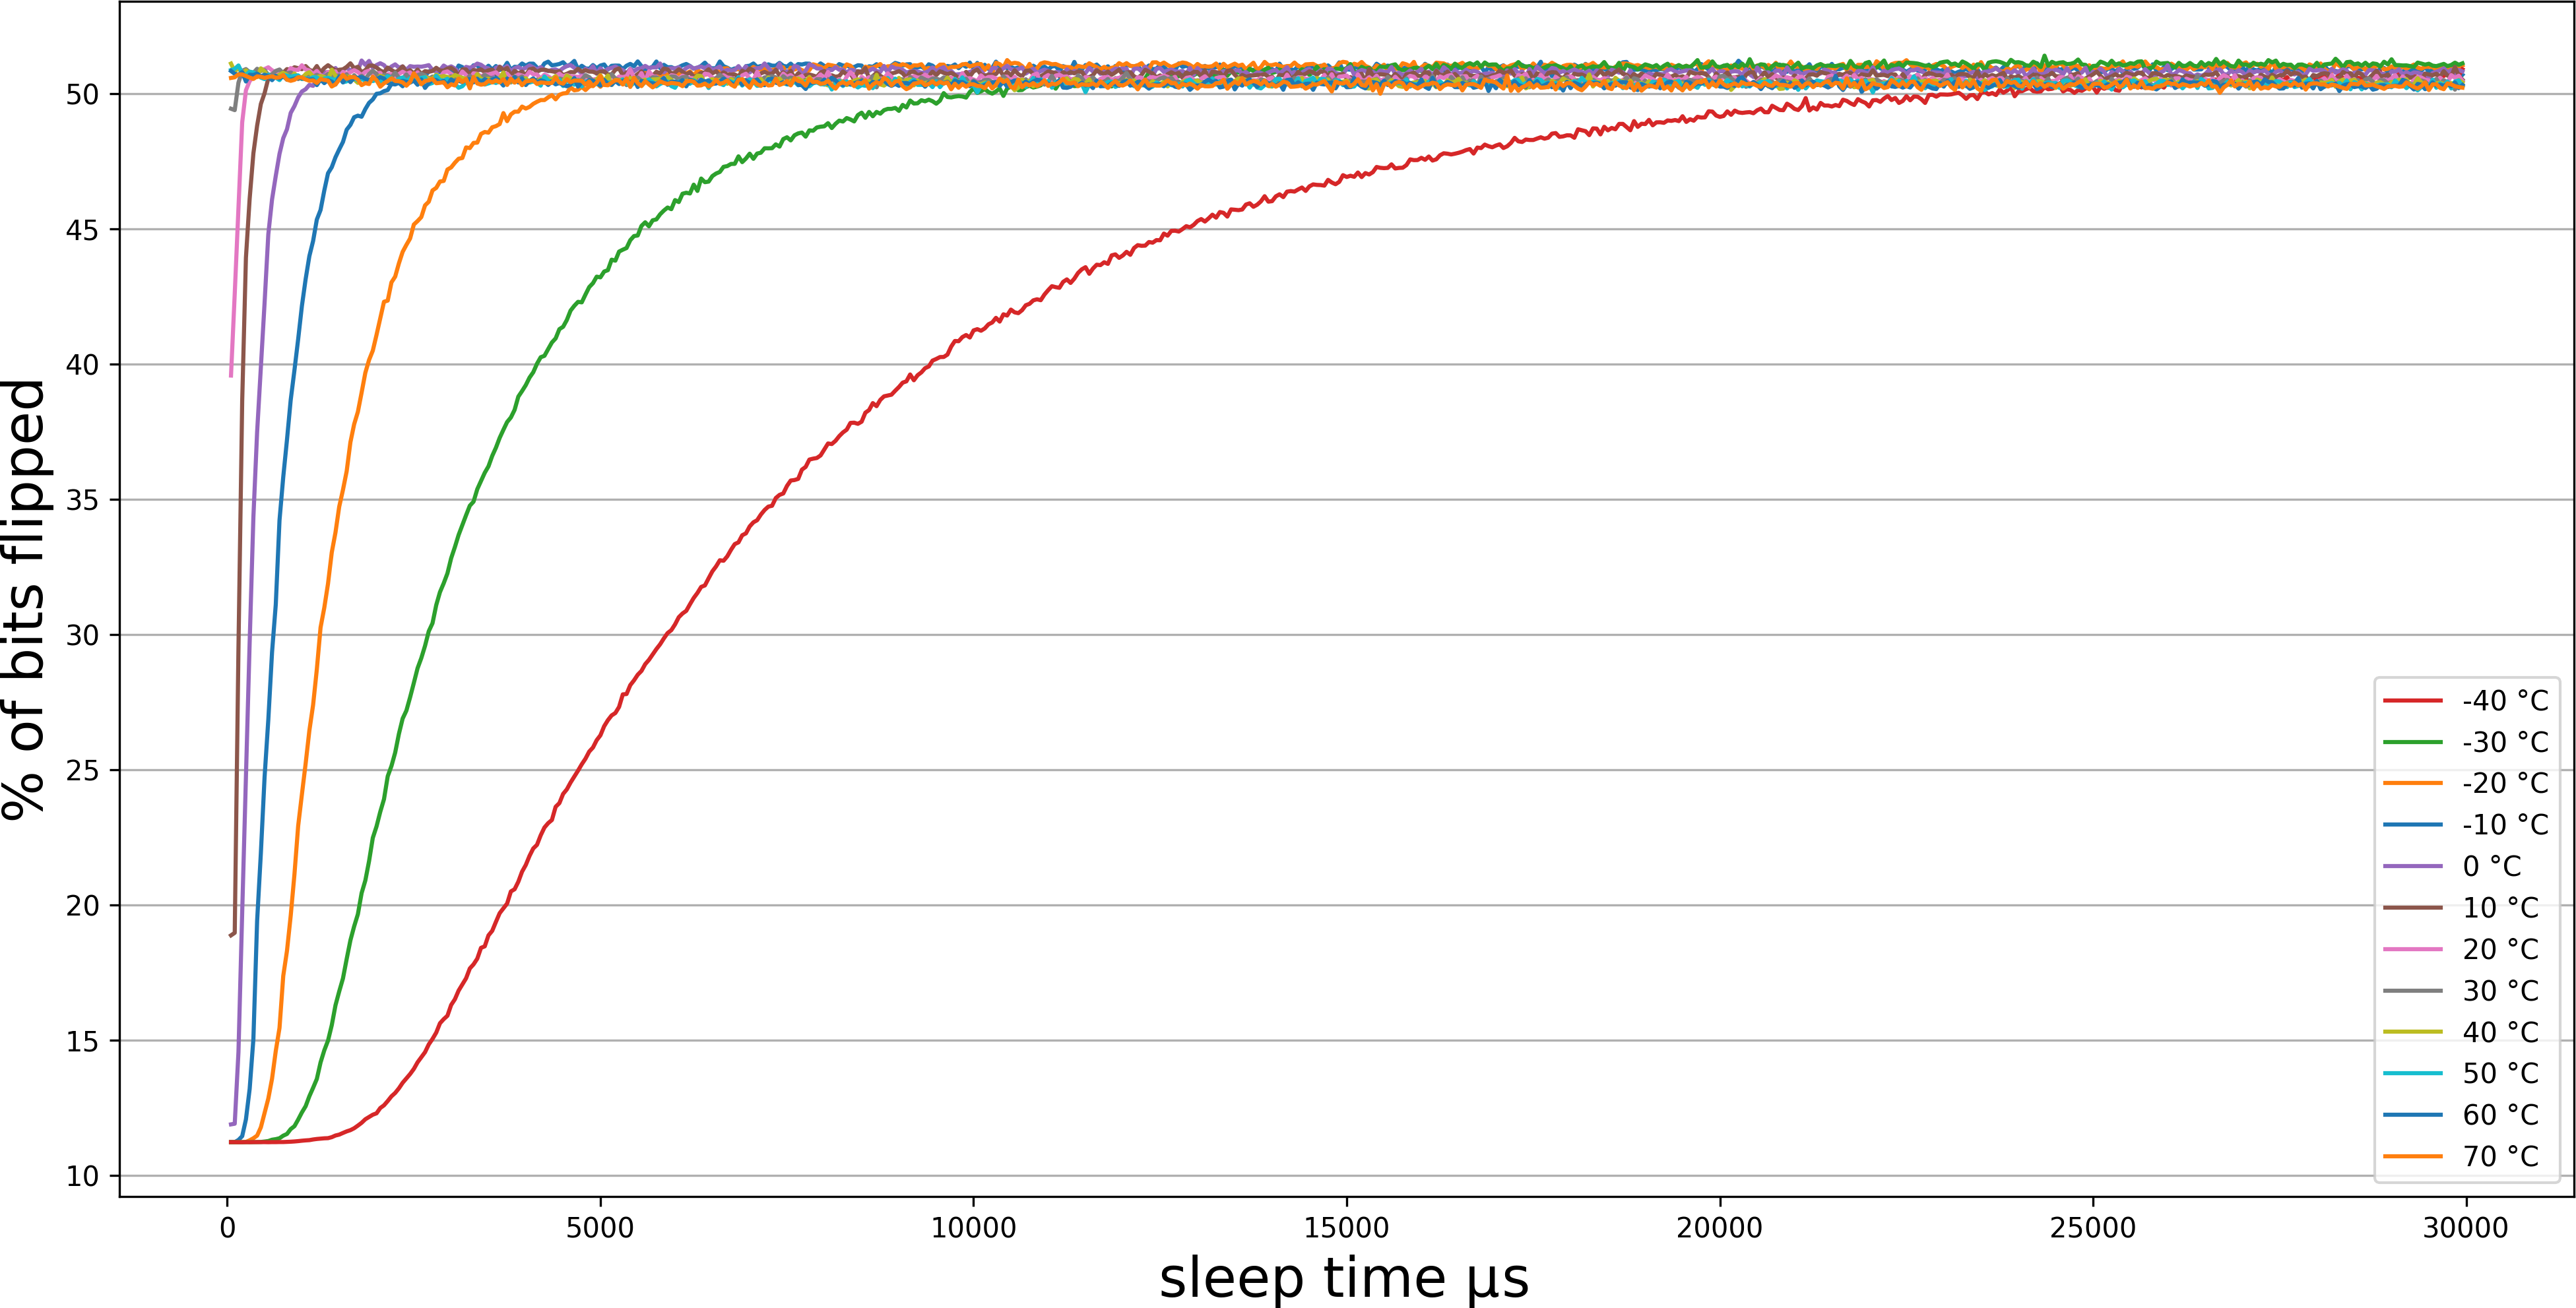
\includegraphics[width=\textwidth]{images/6_across_temps_deep_sleep.png}
    \caption{Percentage of flipped bits of MCU 6 across a range of temperatures (deep sleep method).}
    \label{fig:6_across_temps_deep_sleep}
\end{figure}
\subsection{PUF evaluation parameters}\label{sec:deepsleep_evaluation}

The \gls{puf} responses needed for the calculation of the evaluation parameters were obtained by the deep sleep power-control method. The responses were chosen to be 4 KB bit strings of the internal \gls{sram} 2 startup values. The turn off interval was set to 100 000 $\mu{}S$ since the maximal \emph{fade-out time} of memory was found to be 50 000 $\mu{}S$ plus a conservative safety margin. The reference response was calculated using a bitwise average of 1000 measured responses.

\subsubsection*{Uniformity}

Uniformity of all \glspl{mcu} across the whole range of temperatures can be seen in Table~\ref{table:uniformity_deep_sleep}. All of the results are close to the ideal value of 50 \%, though a small bias towards the `1' bit is evident (all of the results are slightly above 50 \%).

\begin{table}[ht!]
    \centering
    \begin{tabular}{c||rrrrrrrrrr}
    \toprule
    \textbf{MCU} & \textbf{-40°C} & \textbf{-30°C} & \textbf{-20°C} & \textbf{-10°C} & \textbf{0°C} & \textbf{10°C} & \textbf{20°C} & \textbf{30°C} & \textbf{50°C} & \textbf{70°C} \\
    \midrule
    1    &  51.46 &  51.33 &  51.14 &  51.01 & 50.90 & 50.75 & 50.70 & 50.67 & 50.59 & 50.54 \\
    2    &  51.55 &  51.43 &  51.25 &  51.06 & 50.94 & 50.82 & 50.67 & 50.63 & 50.56 & 50.53 \\
    3    &  51.09 &  50.97 &  50.84 &  50.72 & 50.60 & 50.47 & 50.20 & 50.18 & 50.19 & 50.22 \\
    4    &  50.66 &  50.62 &  50.49 &  50.31 & 50.22 & 50.19 & 50.17 & 50.15 & 50.08 & 50.00 \\
    5    &  50.96 &  50.83 &  50.72 &  50.58 & 50.49 & 50.38 & 50.38 & 50.33 & 50.27 & 50.22 \\
    6    &  51.19 &  51.06 &  50.90 &  50.82 & 50.71 & 50.61 & 50.46 & 50.37 & 50.30 & 50.28 \\
    7    &  51.01 &  51.02 &  50.95 &  50.85 & 50.73 & 50.68 & 50.54 & 50.49 & 50.40 & 50.37 \\
    8    &  50.95 &  50.86 &  50.73 &  50.61 & 50.47 & 50.37 & 50.23 & 50.16 & 50.01 & 49.94 \\
    9    &  51.54 &  51.36 &  51.24 &  51.14 & 51.03 & 50.91 & 50.61 & 50.53 & 50.39 & 50.40 \\
    10   &  51.37 &  51.18 &  51.03 &  50.89 & 50.78 & 50.68 & 50.50 & 50.48 & 50.36 & 50.37 \\
    11   &  51.63 &  51.54 &  51.40 &  51.28 & 51.13 & 51.06 & 50.86 & 50.86 & 50.81 & 50.81 \\
    12   &  51.56 &  51.40 &  51.23 &  51.06 & 50.93 & 50.77 & 50.57 & 50.42 & 50.27 & 50.24 \\
    13   &  50.81 &  50.71 &  50.60 &  50.55 & 50.50 & 50.48 & 50.42 & 50.34 & 50.22 & 50.15 \\
    14   &  50.26 &  50.17 &  50.11 &  50.11 & 50.03 & 50.03 & 50.02 & 50.05 & 50.14 & 50.22 \\
    15   &  51.55 &  51.45 &  51.36 &  51.32 & 51.26 & 51.16 & 51.08 & 50.98 & 50.79 & 50.64 \\
    16   &  52.43 &  52.31 &  52.24 &  52.18 & 52.07 & 51.89 & 51.81 & 51.66 & 51.26 & 50.92 \\
    \textbf{mean} &  51.25 &  51.14 &  51.01 &  50.91 & 50.80 & 50.70 & 50.58 & 50.52 & 50.42 & 50.37 \\
    \bottomrule
    \end{tabular}
    \captionsetup{justification=centering,margin=0.5cm}
    \caption{Uniformity (\%) across all MCUs and temperatures (deep sleep method).}
    \label{table:uniformity_deep_sleep}
\end{table}

\subsubsection*{Reliability}

Reliability values of all \gls{mcu} in different temperatures are displayed in Table~\ref{table:reliability_deep_sleep}. The reference response was calculated at 20 °C.

The best reliability is achieved at 20 °C since the reference response was calculated at this temperature. Reliability starts to decrease in different temperatures. The decrease is proportional to the distance from the 20 °C of the reference response. However, the values are still quite close to the ideal 100 \% and they only rarely fall under 90 \% (only at -40 °C).

\begin{table}[ht!]
    \centering
    \begin{tabular}{c||rrrrrrrrrr}
    \toprule
    \textbf{MCU} & \textbf{-40°C} & \textbf{-30°C} & \textbf{-20°C} & \textbf{-10°C} & \textbf{0°C} & \textbf{10°C} & \textbf{20°C} & \textbf{30°C} & \textbf{50°C} & \textbf{70°C} \\
    \midrule
    1    &  90.36 &  91.60 &  92.80 &  93.99 & 95.03 & 95.62 & 96.13 & 95.77 & 94.47 & 92.99 \\
    2    &  91.57 &  92.53 &  93.49 &  94.43 & 95.34 & 96.04 & 96.59 & 96.16 & 94.61 & 93.04 \\
    3    &  90.19 &  91.39 &  92.55 &  93.67 & 94.76 & 95.53 & 96.15 & 95.72 & 94.17 & 92.55 \\
    4    &  90.78 &  91.97 &  93.10 &  94.10 & 95.02 & 95.60 & 96.10 & 95.74 & 94.39 & 92.90 \\
    5    &  90.72 &  91.81 &  92.93 &  94.05 & 95.10 & 95.79 & 96.28 & 95.90 & 94.57 & 93.15 \\
    6    &  90.98 &  92.23 &  93.40 &  94.44 & 95.27 & 95.80 & 96.21 & 95.91 & 94.75 & 93.44 \\
    7    &  90.29 &  91.39 &  92.55 &  93.67 & 94.73 & 95.49 & 96.03 & 95.68 & 94.24 & 92.40 \\
    8    &  90.81 &  91.91 &  93.03 &  94.10 & 95.02 & 95.67 & 96.16 & 95.72 & 94.14 & 92.26 \\
    9    &  90.91 &  91.98 &  92.96 &  93.96 & 94.92 & 95.67 & 96.28 & 95.85 & 94.13 & 92.40 \\
    10   &  90.01 &  91.21 &  92.43 &  93.68 & 94.84 & 95.61 & 96.11 & 95.73 & 94.27 & 92.54 \\
    11   &  89.87 &  91.19 &  92.56 &  93.93 & 95.07 & 95.80 & 96.24 & 95.88 & 94.60 & 93.24 \\
    12   &  90.82 &  91.96 &  93.10 &  94.20 & 95.19 & 95.85 & 96.28 & 95.93 & 94.51 & 92.83 \\
    13   &  90.83 &  91.95 &  93.12 &  94.29 & 95.34 & 96.06 & 96.34 & 95.93 & 94.41 & 92.87 \\
    14   &  90.70 &  91.91 &  93.17 &  94.34 & 95.35 & 95.94 & 96.14 & 95.70 & 94.27 & 92.67 \\
    15   &  90.21 &  91.46 &  92.66 &  93.81 & 94.91 & 95.72 & 96.01 & 95.61 & 94.15 & 92.46 \\
    16   &  89.82 &  91.02 &  92.25 &  93.52 & 94.79 & 95.83 & 96.26 & 95.64 & 93.16 & 90.24 \\
    \textbf{mean} &  90.55 &  91.72 &  92.88 &  94.01 & 95.04 & 95.75 & 96.21 & 95.80 & 94.30 & 92.62 \\
    \bottomrule
    \end{tabular}
    \captionsetup{justification=centering,margin=0.5cm}
    \caption{Reliability (\%) across all MCUs and temperatures (deep sleep method).}
    \label{table:reliability_deep_sleep}
\end{table}

\subsubsection*{Uniqueness}

Uniqueness for all \glspl{mcu} across the range of different temperatures is shown in Table~\ref{table:uniqueness_deep_sleep}. The results hover just under the ideal value of 50 \% for all temperatures.

\begin{table}[ht!]
    \centering
    \begin{tabular}{cc}
        \textbf{Temperature °C} & \textbf{Uniqueness \%} \\
    \toprule
    -40  & 49.37 \\
    -30  & 49.41 \\
    -20  & 49.45 \\
    -10  & 49.49 \\
    0    & 49.51 \\
    10   & 49.56 \\
    20   & 49.61 \\
    30   & 49.63 \\
    40   & 49.66 \\
    50   & 49.68 \\
    60   & 49.70 \\
    70   & 49.73 \\
    \textbf{mean} & 49.57 \\
    \bottomrule
    \end{tabular}
    \captionsetup{justification=centering,margin=0.5cm}
    \caption{Uniqueness (\%) across all MCUs and temperatures (deep sleep method).}
    \label{table:uniqueness_deep_sleep}
\end{table}

\subsection{Summary}

The presented experiments show very good results across the whole tested range of temperatures. Additionally, the deep sleep functionality is available to all microcontrollers in the ESP32 family. This power-control method is therefore not restricted only to a particular subset of models.

On the other hand, the deep sleep power-control method is especially time-consuming (in comparison to the \gls{rtc} \gls{sram} method). This is mainly due to the need to go through the whole booting process. Obtaining the response can take up to several tenths of seconds, depending on the application size and speed of the connected flash memory. Moreover, most of the device state is inevitably lost during deep sleep. The application must save all data it does not want to lose to either the FAST or SLOW \gls{rtc} \gls{sram} (the only memory regions not turned off). Although, they together only provide 16 KB of space

%--------------------------------
\section{PUF response data visualization} % TODO how to name this section?
%--------------------------------

The above-described experiments and evaluation parameters only looked at the response data globally and reduced the entire response bit string to a single number. As will become clear, it can be useful to look at the data more locally. Therefore the following visualization is presented.

The whole 4 KB \gls{puf} response is arranged bit by bit to a $256 \times 128$ grid. Black bits represent the `0' state and white bits represent the `1' state. This visualization of 4 responses from different \glspl{mcu} can be seen in Figure~\ref{fig:puf_response_visualization}. The first two responses were obtained using the deep sleep method and the last two using the \gls{rtc} \gls{sram} method.

The response from \gls{mcu} 1 (\ref{fig:mcu_1}) looks as expected, the bits are arranged in a random-looking pattern\footnote{This, of course, is not proof that the bits really are random}. However, the other responses show strange stripes. Every 32 bits the startup bias of memory cells towards a certain state flips. This results in this stripe-looking pattern. The previous experiments did not reveal this behavior (mainly uniformity), as the overall number of  `0' and `1' bits stays the same globally.

Both power-control methods produce the same result. Additionally, some of the \glspl{mcu} do not exhibit this behavior at all (\ref{fig:mcu_1}), some of them show only a slight `stripe-like' bias (\ref{fig:mcu_13},~\ref{fig:mcu_3}), and some are affected in a lot (\ref{fig:mcu_11}).

\begin{figure}[ht!]
        \centering
        \captionsetup{justification=centering,margin=0.5cm}
        \begin{subfigure}[b]{0.475\textwidth}
            \centering
            
\includegraphics[width=\textwidth]{images/1_response_sleep.png}
            \caption{MCU 1 (deep sleep method)}    
            \label{fig:mcu_1}
        \end{subfigure}
        \hfill
        \begin{subfigure}[b]{0.475\textwidth}  
            \centering 
            
\includegraphics[width=\textwidth]{images/13_response_sleep.png}
            \caption{MCU 13 (deep sleep method)}    
            \label{fig:mcu_13}
        \end{subfigure}
        \vskip 1.75mm
        \begin{subfigure}[b]{0.475\textwidth}   
            \centering 
            
\includegraphics[width=\textwidth]{images/11_response_rtc.png}
            \caption{MCU 11 (RTC SRAM method)}    
            \label{fig:mcu_11}
        \end{subfigure}
        \hfill
        \begin{subfigure}[b]{0.475\textwidth}   
            \centering 
            
\includegraphics[width=\textwidth]{images/3_response_rtc.png}
            \caption{MCU 3 (RTC SRAM method)}    
            \label{fig:mcu_3}
        \end{subfigure}
        \caption{Visualization of PUF responses from different MCUs.} 
        \label{fig:puf_response_visualization}
\end{figure}

One edge case was also revealed. \Gls{mcu} 16 exhibited different behavior from all of the other \glspl{mcu}. Its `stripes' are 256 bits wide. In order to visualize this, the grid was reshaped into a $512 \times 64$ configuration which is shown in Figure~\ref{fig:16_response_sleep}.

However, only the \gls{rtc} \gls{sram} method shows this wide stripe behavior. This is probably not due to the different power-state control of memory, but rather because a different memory region is used for the response extraction.

\begin{figure}[ht!]
    \centering
    \captionsetup{justification=centering,margin=0.5cm}
    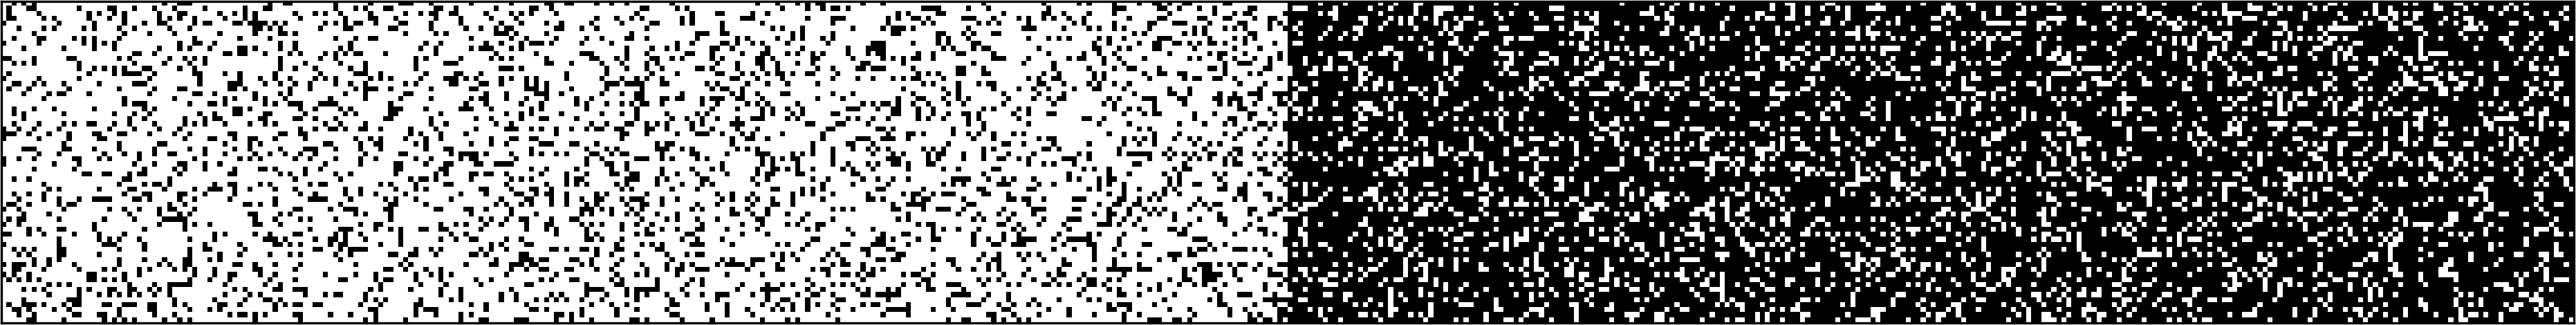
\includegraphics[width=\textwidth]{images/16_response_sleep.png}
    \caption{Visualization of PUF response from MCU 16 (RTC SRAM method).}
    \label{fig:16_response_sleep}
\end{figure}

This behavior is most likely caused by the internal design of the \gls{sram} circuit and there is no way to prevent it. This explanation unfortunately cannot be confirmed as the ESP32 chip schematics are not available. It is, however, clear that the entropy of the resulting \gls{puf} response is reduced because of this behavior.


%---------------------------------------------------------------
\chapter{Reliable PUF response extraction}\label{sec:response_extraction} % TODO should this be its own section or part of the previous one?
%---------------------------------------------------------------

Since \gls{sram} \glspl{puf} are classified as weak (they do not have a large challenge-response pair set), their main use is for cryptographic key generation. The keys need to be reconstructed without error, otherwise the cryptographic algorithms that use the keys will not work. Therefore, methods of reliable response extraction are used to stabilize the \gls{puf} response.

In this chapter, stable bit preselection and \gls{ecc} techniques are used on top of the designed memory power-control methods in order to stabilize the responses of the ESP32 \gls{sram} \gls{puf}. Then, a \gls{puf} design that combines the two power-control methods is presented. At the end, the enrollment process of key generation is discussed and the resulting \gls{sram} \gls{puf} based key generation is tested on all \glspl{mcu} at different operating temperatures.

%--------------------------------
\section{Stable bit preselection}
%--------------------------------

Stable bit preselection consists of two steps. First, during the enrollment phase, the stable bits are selected and a stable bit mask is created. The mask is then saved to a non-volatile memory of the device. When a \gls{puf} response needs to be reconstructed, the mask is loaded and the unstable bits are discarded.

Direct bit preselection was used to obtain the stable bits. Other methods that try to preselect stable bits exist, such as the indirect preselection method described in Section~\ref{sec:indirect_bit_preselection}. However, the discussed stability test which measures the stabilization time of each memory cell, cannot be used for our \gls{puf} implementation. The deep sleep method of memory power-control does not enable turn off intervals of less than 1000 $\mu{}S$. Thus, it is not possible to carry out the test accurately.

\subsubsection*{Stable bit mask creation}

The stable bit mask is created by measuring a \gls{puf} response multiple times. An average startup value $\bar{x}$ of each bit is then calculated from the responses. Then, a threshold value, called the error rate $E_r$, needs to be selected. Bits with average value $\bar{x} \leq E_r$ (stable `0') or $\bar{x} \geq (1-E_r)$ (stable `1') are declared as stable.

Two techniques were used to generate the stable bit mask. First, 1000 measurements of the \gls{puf} response were taken in 20 °C and the mask was created using the above-described method.

The second technique was inspired by~\cite{Hanova2020}. Twelve different intermediate masks were created, each from 1000 measurements of the \gls{puf} response. The measurements for each mask were captured in different operating conditions.\footnote{The temperatures of -40, -30, -20, -10, 0, 10, 20, 30, 40, 50, 60 and 70 °C were used for the twelve masks.} Then, the final mask was calculated as a bitwise logical AND from the twelve intermediate masks---a bit is declared stable if it is stable at all twelve operating temperatures.

\subsubsection*{Results}

Table~\ref{table:stable_bits} shows the percentage of stable bits found in a 4 KB sample \gls{puf} response for all \glspl{mcu}. Three different error rates were chosen, 10 \%, 1 \% and 0.1 \%. As expected, lower error rate reduces the number of stable bits. Moreover, the temperature range mask (created by the second technique) further reduced the percentage of stable bits by about 17 \% compared to the 20 °C mask. Only the results for the deep sleep method of power-control are presented, as the temperature range mask cannot be used for the \gls{rtc} \gls{sram} method (because of the memory freezing effect). The error rate of 0.1 \% was chosen for the \gls{sram} \gls{puf} implementation as it provides the best reliability with only a minor reduction of available bits.

\begin{table}[ht!]
    \centering
    \begin{tabular}{c||ccc|ccc}
    \multicolumn{1}{c}{} & \multicolumn{3}{c}{20 °C mask} & \multicolumn{3}{c}{Temperature range mask} \\
    \toprule
    \textbf{MCU} &  \textbf{10 \%} &  \textbf{1.0 \%} &  \textbf{0.1 \%} &  \textbf{10 \%} &  \textbf{1.0 \%} &  \textbf{0.1 \%} \\
    \midrule
    1    &   87.37 &  77.32 &  71.24 &    72.39 &   62.87 &   56.43 \\
    2    &   87.56 &  77.66 &  71.58 &    72.79 &   63.05 &   56.67 \\
    3    &   87.94 &  78.60 &  72.82 &    73.54 &   64.29 &   58.24 \\
    4    &   87.55 &  77.50 &  71.34 &    72.31 &   62.90 &   56.76 \\
    5    &   87.75 &  77.91 &  71.82 &    74.41 &   64.91 &   58.47 \\
    6    &   87.89 &  78.09 &  72.11 &    73.18 &   63.72 &   57.80 \\
    7    &   88.11 &  78.97 &  72.93 &    73.93 &   64.56 &   58.34 \\
    8    &   87.58 &  77.89 &  72.04 &    73.93 &   64.59 &   58.52 \\
    9    &   88.03 &  78.49 &  72.38 &    74.12 &   64.55 &   58.25 \\
    10   &   87.70 &  77.88 &  71.83 &    73.43 &   63.84 &   57.54 \\
    11   &   89.07 &  80.03 &  74.57 &    75.36 &   66.24 &   60.24 \\
    12   &   87.56 &  77.60 &  71.51 &    72.64 &   62.93 &   56.76 \\
    13   &   88.22 &  79.13 &  73.32 &    73.89 &   65.01 &   59.09 \\
    14   &   87.50 &  77.67 &  71.80 &    73.04 &   63.68 &   57.60 \\
    15   &   87.30 &  77.18 &  71.51 &    72.42 &   62.95 &   56.71 \\
    16   &   88.00 &  78.59 &  72.84 &    70.15 &   61.36 &   55.54 \\
    \textbf{mean} &   87.82 &  78.16 &  72.23 &    73.22 &   63.84 &   57.68 \\
    \bottomrule
    \end{tabular}
    \captionsetup{justification=centering,margin=0.5cm}
    \caption{Percentage of stable bits across all MCUs. Three different error rates (10 \%, 1 \% and 0.1 \%) and two stable bit selection methods were used.}
    \label{table:stable_bits}
\end{table}

Table~\ref{table:reliability_stable_bits} shows reliability of \gls{puf} responses at different operating temperatures and for all \glspl{mcu}. The reference response was obtained at 20 °C and only the stable bits of the responses were selected using the 20 °C mask. The table shows results using the deep sleep power-control method, but the \gls{rtc} \gls{sram} method shows nearly identical results above -10 °C.

The best reliability is observed at 20°C, since this is the temperature the reference and stable bit mask were calculated at. With increasing distance from 20°C, the reliability reduces. However, reliability was increased significantly thanks to the stable bit preselection. Reliability results without the preselection can be found in Table~\ref{table:reliability_deep_sleep}.

\begin{table}[ht!]
    \centering
    \begin{tabular}{c||rrrrrrrrrr}
    \toprule
    \textbf{MCU} & \textbf{-40°C} & \textbf{-30°C} & \textbf{-20°C} & \textbf{-10°C} & \textbf{0°C} & \textbf{10°C} & \textbf{20°C} & \textbf{30°C} & \textbf{50°C} & \textbf{70°C} \\
    \midrule
    1    &  98.27 &  98.96 &  99.45 &  99.75 & 99.88 & 99.92 & 99.99 & 99.97 & 99.83 & 99.42 \\
    2    &  98.59 &  99.09 &  99.45 &  99.71 & 99.87 & 99.92 & 99.99 & 99.95 & 99.74 & 99.19 \\
    3    &  98.17 &  98.84 &  99.33 &  99.65 & 99.81 & 99.89 & 99.99 & 99.97 & 99.81 & 99.30 \\
    4    &  98.51 &  99.11 &  99.51 &  99.76 & 99.88 & 99.92 & 99.99 & 99.97 & 99.83 & 99.44 \\
    5    &  98.24 &  98.87 &  99.37 &  99.71 & 99.87 & 99.93 & 99.99 & 99.98 & 99.84 & 99.44 \\
    6    &  98.50 &  99.13 &  99.54 &  99.76 & 99.88 & 99.91 & 99.99 & 99.97 & 99.87 & 99.58 \\
    7    &  98.21 &  98.86 &  99.37 &  99.68 & 99.85 & 99.92 & 99.99 & 99.97 & 99.77 & 99.15 \\
    8    &  98.31 &  98.92 &  99.36 &  99.65 & 99.81 & 99.89 & 99.99 & 99.95 & 99.74 & 99.08 \\
    9    &  98.51 &  99.06 &  99.44 &  99.70 & 99.84 & 99.90 & 99.99 & 99.96 & 99.74 & 99.09 \\
    10   &  98.14 &  98.82 &  99.36 &  99.71 & 99.88 & 99.93 & 99.99 & 99.97 & 99.79 & 99.22 \\
    11   &  97.99 &  98.78 &  99.39 &  99.75 & 99.91 & 99.94 & 99.99 & 99.98 & 99.83 & 99.45 \\
    12   &  98.32 &  98.98 &  99.46 &  99.74 & 99.88 & 99.92 & 99.99 & 99.98 & 99.79 & 99.23 \\
    13   &  98.29 &  98.95 &  99.46 &  99.79 & 99.94 & 99.97 & 99.99 & 99.97 & 99.78 & 99.27 \\
    14   &  98.33 &  99.03 &  99.54 &  99.83 & 99.94 & 99.97 & 99.99 & 99.95 & 99.79 & 99.30 \\
    15   &  98.22 &  98.95 &  99.45 &  99.76 & 99.92 & 99.97 & 99.99 & 99.97 & 99.80 & 99.30 \\
    16   &  97.41 &  98.20 &  98.88 &  99.42 & 99.80 & 99.96 & 99.99 & 99.96 & 99.33 & 97.60 \\
    \textbf{mean} &  98.25 &  98.91 &  99.40 &  99.71 & 99.87 & 99.93 & 99.99 & 99.97 & 99.77 & 99.19 \\
    \bottomrule
    \end{tabular}
    \captionsetup{justification=centering,margin=0.5cm}
    \caption{Reliability (\%) across all MCUs and temperatures (deep sleep method). Preselected stable bits with error rate of 0.1 \% were used.}
    \label{table:reliability_stable_bits}
\end{table}

Reliability table using the temperature range mask is not presented, as the reliability values for all temperatures and \glspl{mcu} are above 99.99 \%. This technique thus increases reliability significantly. Unfortunately, the creation of the temperature mask requires a controlled temperature environment and takes much longer, making the enrollment phase more difficult and costly. On the other hand, the 20 °C mask can be calculated easily (the exact value of temperature does not matter and room temperature suffices).

% poznamka ze po selekci bitu stale vypadaji uniformity, reliability (mnohem lepsi lol, asi ukazat?) a uniqueness dobre
% mozna pridat jednu tabulku s reliability pro 20 stupnu masku a pro vsechny masku?
% pridat tabulku s poctem stabilnich bitu? pri 20 stupnich a pro vsechny a par rucnych error rates
% proc jsem vybral 8bit repetition ecc? binomicka distribucni funkce podle https://idus.us.es/bitstream/handle/11441/58931/Baturone_TIFS_2015_PersonalCopy.pdf?sequence=1&isAllowed=y

%--------------------------------
\section{Error correction code}\label{sec:ecc}
%--------------------------------

Stable bit preselection managed to increase reliability significantly. However, for successful key reconstruction the reliability must be 100 \% as only a single bit flip renders the key unusable. For this reason, \glspl{ecc} are used as an additional method to reduce the noise of the \gls{puf} responses.

One method of applying an \gls{ecc} to the \gls{puf} responses is called the code-offset construction. In the enrollment phase, a reference response needs to be chosen. A random code word of the used code is then subtracted from the response and the results are stored in a non-volatile memory. This data is called the helper data. During the key reconstruction phase, a new, potentially noisy \gls{puf} response is generated. Helper data are retrieved from memory and added to the response, creating the code word of the \gls{ecc}. This (also potentially noisy) code word is then decoded by the \gls{ecc}, correcting the errors.\cite{Sven2015}\cite{Dodis2008}

The repetition code of length 8 was chosen for the \gls{sram} \gls{puf} implementation. It is very simple to implement and the encoding and decoding operations are extremely fast, because the code words are byte-sized. It is capable of correcting up to 3 errors and can detect up to 4 errors per byte.

The above-described code-offset construction is used for extracting the key. Addition and subtraction are both realized as the logical XOR operation. Each eight bits of the reference response are XORed with a code word chosen by the first bit of the eight, generating the helper data.\footnote{This \gls{ecc} only has two code words, 00000000 and 11111111.} During reconstruction, the helper data is again XORed with the new noisy \gls{puf} response and the resulting code words are decoded using a majority bit. This process is illustrated in Figure~\ref{fig:ecc_diagram}, by using a shorter repetition code of length 5.

\begin{figure}[ht!]
    \centering
    \captionsetup{margin=0.5cm}
    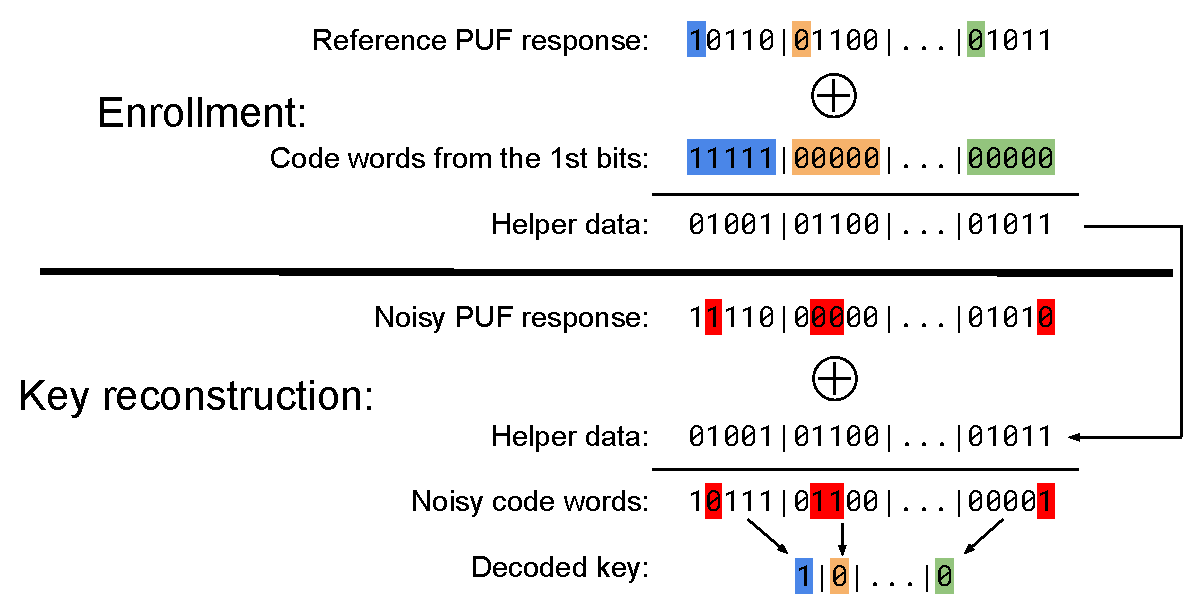
\includegraphics[width=0.85\textwidth]{images/ecc_diagram.pdf}
    \caption[An example of enrollment and key reconstruction phases using repetition code of length 5.]{An example of enrollment and key reconstruction phases using repetition code of length 5. Red bits are the error bits (flipped compared to the reference response), other colors represent individual bits of the key.\cite{Kodytek2017}}
    \label{fig:ecc_diagram}
\end{figure}

Since the \gls{ecc} can correct only a limited number of errors, the \gls{puf} response can be too noisy for the key to be properly reconstructed. The probability of this happening can be modeled using the binomial distribution. Assuming that all response bits are independent and have the same probability of error\footnote{Error is understood as a bit flip compared to the reference \gls{puf} response.}, the probability of successfully decoding a single code word can be calculated using the binomial cumulative distribution function:\cite{Iluminada2015}\cite{Christoph2008}

\begin{equation}\label{eq:binomial_cdf}
    F(k, n, p) = \sum_{i=0}^{k}\binom{n}{i}p^{i}(1-p^{n-i})
\end{equation}

$N$ is the size of the code word, $k$ is the maximum number of corrected errors and $p$ is the probability of a single bit error. The Equation~\ref{eq:binomial_cdf} only calculates the probability of successfully decoding a single code word which gives us only one bit of the key (because of the repetition code). To obtain the whole key, each bit is reconstructed independently and thus the probability of successful reconstruction $P_{\textrm{succ}}$ can be calculated using the Equation~\ref{eq:succ_probability}, where $B$ is the number of bits of the key (or equivalently the number of bytes of the reference response).

\begin{equation}\label{eq:succ_probability}
    P_{\textrm{succ}} = F(k, n, p)^{B} 
\end{equation}

For our case of the repetition code of length 8, maximum of three errors can be corrected in 8 bits. Therefore $n = 8$, $k = 3$ and $p$ can be estimated by the intra-Hamming distance or $1 - \textrm{reliability}$.\cite{Iluminada2015} $B$ was chosen as $4096 \times 0.7223 \approx 2958$: a 4 KB response and 72.23 \% of stable bits (a mean value across all \glspl{mcu} using the 20°C mask).

\cite{Christoph2008} states that key reconstruction should achieve $P_{\textrm{succ}}$ of at least $1 - 10^{-6}$ or less than one error in a million. In order to meet this requirement, the value of reliability must be greater than 99.85 \% according to the equations above. Using this knowledge, it can be concluded that a \gls{sram} \gls{puf} implementation using the 20°C stable bit mask and deep sleep power-control method is suitable only in temperatures between approximately 0 and 40 °C (see Table~\ref{table:reliability_stable_bits}). A stronger \gls{ecc} needs to be used to extend the temperature range. As the temperature range mask achieves reliability greater than 99.99 \% in all temperatures, it is suitable to be used in all tested conditions with this \gls{ecc}.

This model further calculates that $P_{\textrm{succ}}$ is 98.181 \% (or about 1 error in 55) for -40 °C and 99.913 \% (or about 1 error in 1150) for 70 °C.\footnote{Again, using the 20 °C stable bit mask and deep sleep power-control method.} However, the real-world testing showed considerably lower number of errors in key reconstructions than was predicted by this model. Results from this testing can be found in Chapter~\ref{sec:testing}

%--------------------------------
\section{Combining power control methods}
%--------------------------------

%--------------------------------
\section{Reliability testing}\label{sec:testing}
%--------------------------------

% TODO nejaka tabulka s prumernym mnozstvim detekovanych chyb ECC kodu a kolikrat se rekonstruovalo dobre?
% TODO rict, ze je dobry zahashovat nebo neco udelat kvuli pruhum s odpovedi pred tim nez se pouzije jako klic? z Sven2015

%---------------------------------------------------------------
\chapter{ESP32 SRAM PUF library}\label{sec:puflib}
%---------------------------------------------------------------

The presented \gls{sram} \gls{puf} design with combined power-control and stable \gls{puf} response reconstruction using repetition \gls{ecc} and stable bit preselection was implemented in a library called esp32\_puflib. 

The esp32\_puflib library is implemented as an ESP-IDF component. Components are modular pieces of standalone code. They are compiled as a static library and then linked into the main project by the toolchain. The ESP-IDF component manager makes it easy to add existing components to the main project.~\cite{espidf2022}

%--------------------------------
\section{Enrollment}
%--------------------------------

In order to be able to reconstruct the \gls{puf} responses properly, the device needs to be enrolled first. This means creating the stable bit mask, calculating the \gls{ecc} helper data and saving them to non-volatile memory. Two different enrollment procedures were implemented, in-device enrollment and external enrollment.

\subsubsection*{In-device enrollment}

In the in-device enrollment, the ESP32 microcontroller does all of the needed calculations by itself. It is performed by the \lstinline{provision_puf} function. This method of enrollment is very straightforward to use (just a function call).

Unfortunately, the stable bit mask can be calculated only at one operating temperature (which results in erroneous response reconstructions at extreme temperatures). Furthermore, the in-device enrollment process is lengthy. A stable bit mask created from 1000 \gls{puf} measurements takes about 40 minutes to calculate---each measurement executes the deep sleep restart and a write the non-volatile flash memory to save the results. Thus this method also increases the wear of the flash memory.

\subsubsection*{External enrollment}

In the external enrollment, the ESP32 sends the \gls{puf} measurements to a server through \gls{uart}. The measurements can be repeated in different operating temperatures to increase stability. The server then calculates the stable bit mask and the \gls{ecc} helper data from the received measurements. The results are then exported as a \gls{nvs} partition\footnote{\gls{nvs} is an ESP-IDF library for saving data to flash memory.} and uploaded to the device.

This method is quicker (with 1000 \gls{puf} measurements the process takes about 5 minutes) and enables measurements in different operating conditions, increasing stability significantly. On the other hand, it requires a more elaborate setup (serial connection with the server that runs the enrollment scripts).

%--------------------------------
\section{Example of usage}
%--------------------------------

The minimal working example code of the esp32\_puflib library is shown in Code listing~\ref{lst:puflib_example}. The code initializes the library and reconstructs the \gls{puf} response. If the \gls{rtc} \gls{sram} method did not succeed in the reconstruction, the deep sleep method is used. In this case, the application needs to save its state and is then restarted (line 17). The \gls{puf} response is then printed to \lstinline{stdout} and erased from memory.

After reconstructing the response (either by the \gls{rtc} \gls{sram} method immediately or after restart by the deep sleep method), the library sets global variables with the \gls{puf} response accordingly---\lstinline{PUF_STATE} flag to \lstinline{RESPONSE_READY}, \lstinline{PUF_RESPONSE} to the response data and \lstinline{PUF_RESPONSE_LEN} to response length in bytes.


\begin{lstlisting}[
                   language=C++,
                   caption=Minimal working example of the ESP32\_puflib library,
                   backgroundcolor=\color{white},
                   numbers=left,
                   captionpos=b,
                   style=customc,
                   label=lst:puflib_example
                  ]
#include <stdio.h>
#include <esp_sleep.h>
#include <puflib.h>

void app_main(void) { 
    // needs to be called first in app_main
    puflib_init();
    // provisioning needs to be done only once at the beginning
    provision_puf();

    // condition will be true, if a PUF response is ready
    // (useful after a restart)
    if(PUF_STATE != RESPONSE_READY) {
        bool puf_ok = get_puf_response();
        if(!puf_ok) {
            // the device resets now, SAVE APPLICATION STATE
            get_puf_response_reset();
        }
    }

    // PUF_RESPONSE_LEN is a PUF response length in bytes
    for (size_t i = 0; i < PUF_RESPONSE_LEN; ++i) {
        // PUF_RESPONSE is a buffer with the PUF response
        printf("%02X ", PUF_RESPONSE[i]);
    }

    // erases the PUF response from memory
    clean_puf_response();
}

void RTC_IRAM_ATTR esp_wake_deep_sleep(void) {
    esp_default_wake_deep_sleep();
    // needs to be called somewhere in wake up stub
    puflib_wake_up_stub();
}
\end{lstlisting}


%---------------------------------------------------------------
\chapter*{Conclusion}\label{sec:conclusion}
\phantomsection
\addcontentsline{toc}{chapter}{Conclusion}
%---------------------------------------------------------------

In this thesis, the possibility of implementing a \gls{sram} \gls{puf} on the ESP32 microcontroller was analyzed and a proof of concept solution was implemented. 

First, a description of the concept of a \gls{puf} was provided. \gls{puf} properties, applications, classification and evaluation parameters were described and three \gls{puf} implementations were presented.

A thorough explanation of \gls{sram} \glspl{puf} was given. A discussion on which properties the \gls{sram} \gls{puf} possesses was provided. Then, stable bit preselection methods and the effect of silicon aging were presented and existing research on \gls{sram} \glspl{puf} on the ESP32 platform was summarized. An overview of the ESP32 platform was also provided. The presented theory was used in the \gls{sram} \gls{puf} experiments and implementation in this thesis.

Then, two power-control methods of the \gls{sram} memory were presented, the \gls{rtc} \gls{sram} method and the deep sleep method. To assess the performance of the \gls{sram} \gls{puf} that will use these methods, several experiments were conducted. Data remanence of the \gls{sram} memory and evaluation parameters were analyzed across a range of temperatures. The \gls{rtc} \gls{sram} method showed a surprising effect of memory `freezing' and was found to be suitable for use only at temperatures above about 10 °C. The deep sleep method showed very good results according to the evaluation parameters and data remanence testing. However, it is significantly slower compared to the former method. Additionally, \gls{puf} response visualization revealed an interesting pattern of the uninitialized \gls{sram} data in some \glspl{mcu}, which reduces the entropy of the \gls{puf} responses.

Based on the analyses conducted, a \gls{sram} \gls{puf} implementation with reliable response extraction was designed. Two methods of stable bit preselection were implemented and tested. Then, a simple repetition \gls{ecc} was used to further stabilize the responses. A simple mathematical model of reconstruction success was used to evaluate the reliability of the \gls{puf}. Next, a \gls{puf} design that combines the two power-control methods was presented. By default, the fast \gls{rtc} \gls{sram} method is used, with the slower deep sleep method used as a fallback mechanism. This design was successfully tested on 16 \glspl{mcu} across a range of temperatures.

Finally, the described \gls{sram} \gls{puf} design was implemented in an easy-to-use ESP32 library together with an in-device and external enrollment. The \gls{puf} responses can be used to generate and preserve cryptographic keys safely, increasing the security of the ESP32 platform.

To summarize, all of the goals outlined were accomplished, resulting in interesting findings and a working \gls{sram} \gls{puf} implementation on the ESP32 microcontroller.

\pagebreak

\section*{Future work}
\phantomsection
\addcontentsline{toc}{section}{Future work}

At the end, ideas for possible future research are presented:
\begin{itemize}
    \item test the \gls{puf} responses using more evaluation parameters (such as randomness or bit-aliasing)
    \item use more advanced \glspl{ecc} to achieve greater reliability without the need for sophisticated stable bit preselection
    \item evaluate the behaviour of the \gls{puf} depending on other operating conditions (for example supply voltage)
    \item test the \gls{sram} \gls{puf} implementation on the new RISC-V based ESP32 microcontroller models
    \item apply the reconstructed key to secure communication on ESP32
\end{itemize}

% pro DPR staci jen nastrel
% zopakovat cile, napsat jestli a jak jsem je splnil a future work


\appendix\appendixinit % do not remove these two commands

% \chapter{Attachments}
 % include `appendix.tex' from `text/' subdirectory

\backmatter % do not remove this command

\printbibliography % print out the BibLaTeX-generated bibliography list

\chapter{Obsah přiloženého média}


	\dirtree{%
		.1 readme.txt\DTcomment{stručný popis obsahu média}.
		.1 exe\DTcomment{adresář se spustitelnou formou implementace}.
		.1 src.
		.2 impl\DTcomment{zdrojové kódy implementace}.
		.2 thesis\DTcomment{zdrojová forma práce ve formátu \LaTeX{}}.
		.1 text\DTcomment{text práce}.
		.2 thesis.pdf\DTcomment{text práce ve formátu PDF}.
	}
 % include `medium.tex' from `text/' subdirectory

\end{document}
